\documentclass[12pt]{extarticle}
\usepackage[paperwidth=18in,paperheight=8.5in]{geometry}
\usepackage{amsmath}
\usepackage{hyperref}
\usepackage{multirow}
\usepackage{pdfpages}
\usepackage[utf8]{inputenc}
\title{Kaon mixing: chiral and continuum extrapolations}
\author{R Mukherjee}
\date{\today}
\begin{document}
\maketitle
\tableofcontents
\clearpage
\begin{figure}
\centering
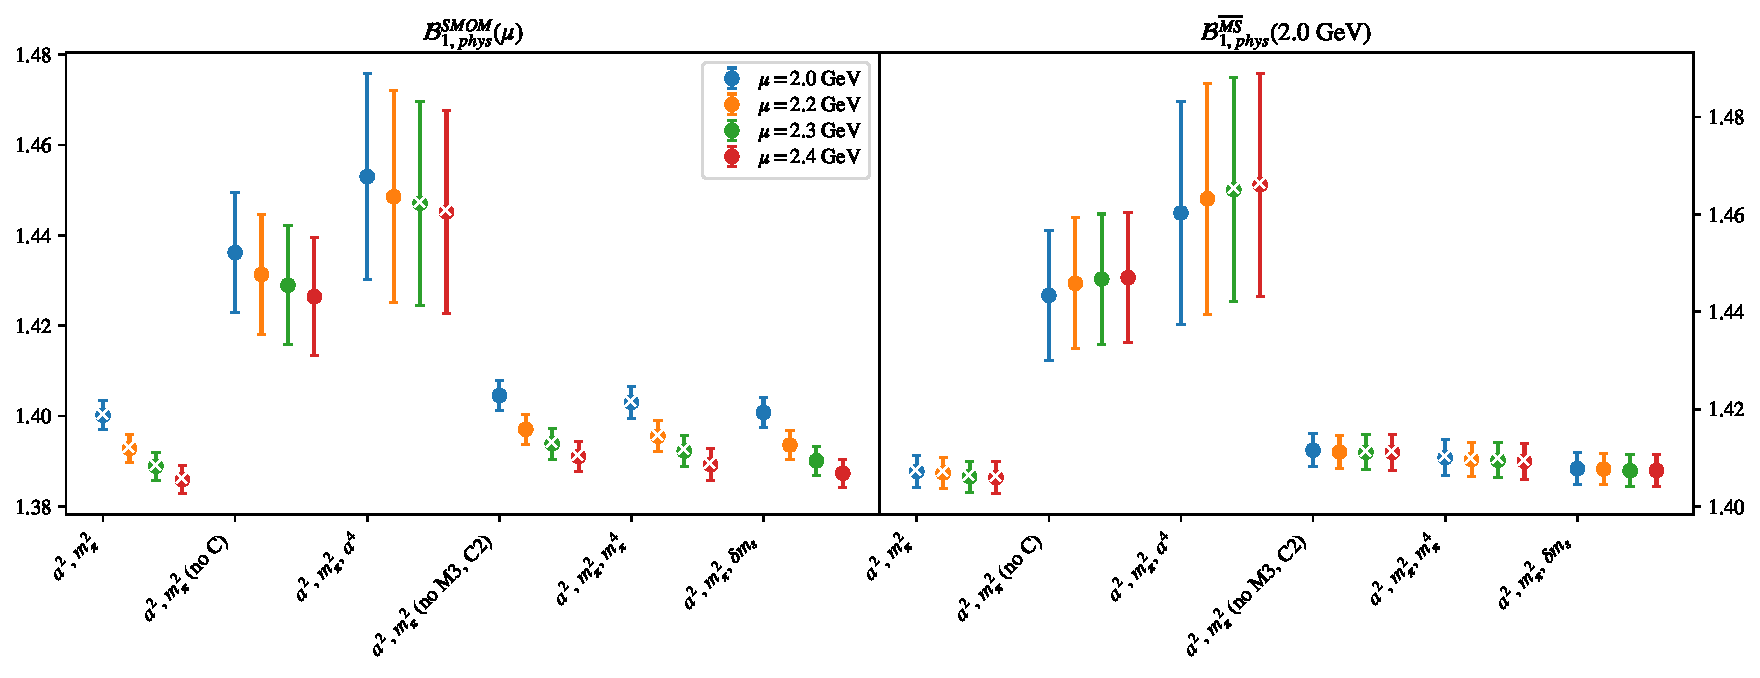
\includegraphics[page=1, width=1.1\textwidth]{VVpAA/NPR/fit_summary_bag.pdf}
\caption{$\mathcal{B}_{1}$\\(left) $\mathcal{B}_{phys}$ in RI/SMOM scheme from fit variations (fits with $p$-value $<0.05$ marked with ``$\times$"). \\(right) $\mathcal{B}_{phys}$ in $\overline{MS}$ computed using $\mathcal{B}^{\overline{MS}} = R^{\overline{MS}\leftarrow SMOM}(2.0)\sigma_{npt}(2.0,\mu) \mathcal{B}^{SMOM}(\mu)$.}
\end{figure}
\clearpage
\begin{figure}
\centering
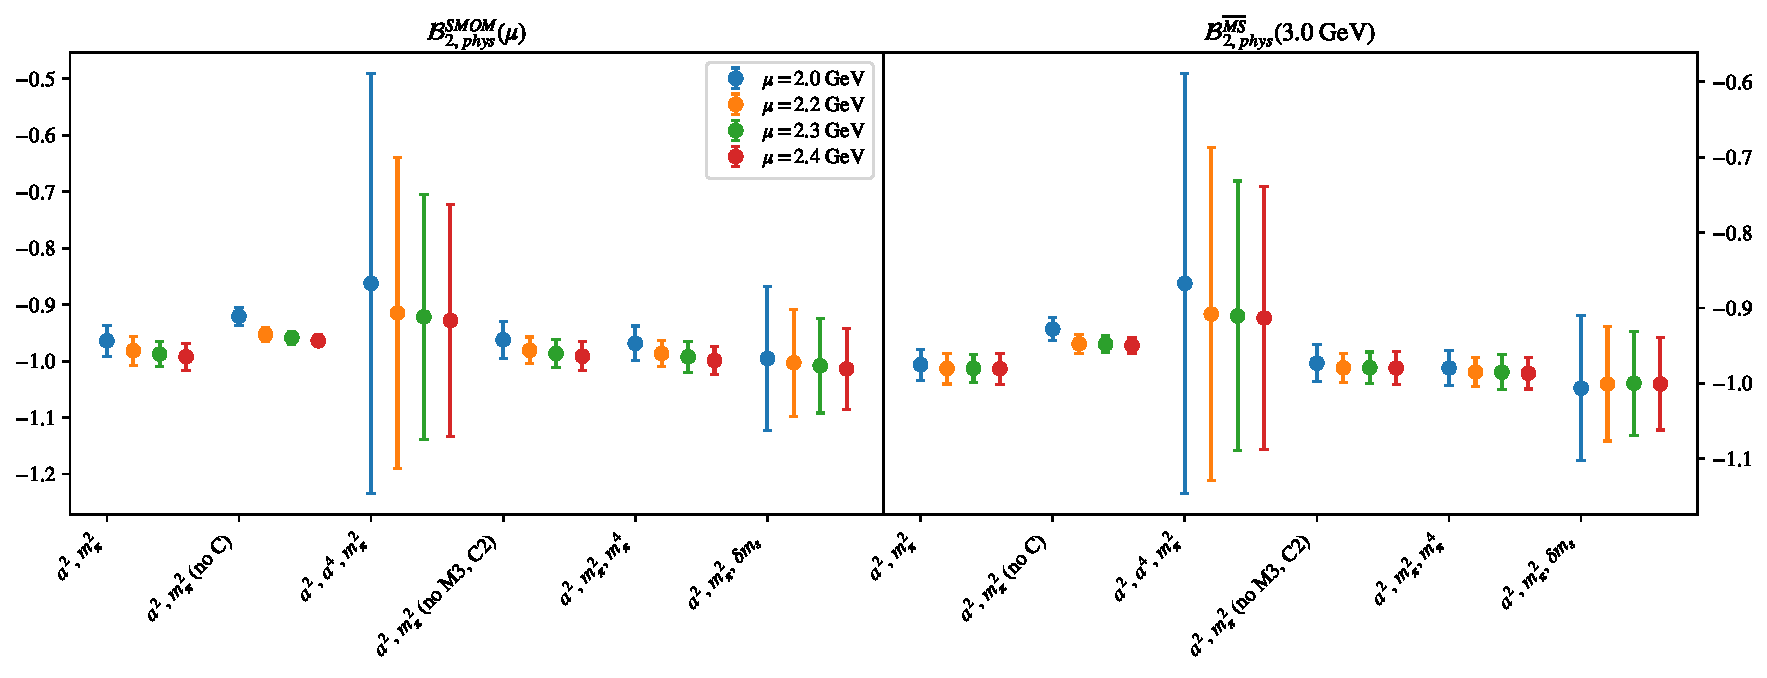
\includegraphics[page=1, width=1.1\textwidth]{VVmAA/NPR/fit_summary_bag.pdf}
\caption{$\mathcal{B}_{2}$\\(left) $\mathcal{B}_{phys}$ in RI/SMOM scheme from fit variations (fits with $p$-value $<0.05$ marked with ``$\times$"). \\(right) $\mathcal{B}_{phys}$ in $\overline{MS}$ computed using $\mathcal{B}^{\overline{MS}} = R^{\overline{MS}\leftarrow SMOM}(3.0)\sigma_{npt}(3.0,\mu) \mathcal{B}^{SMOM}(\mu)$.}
\end{figure}
\clearpage
\begin{figure}
\centering
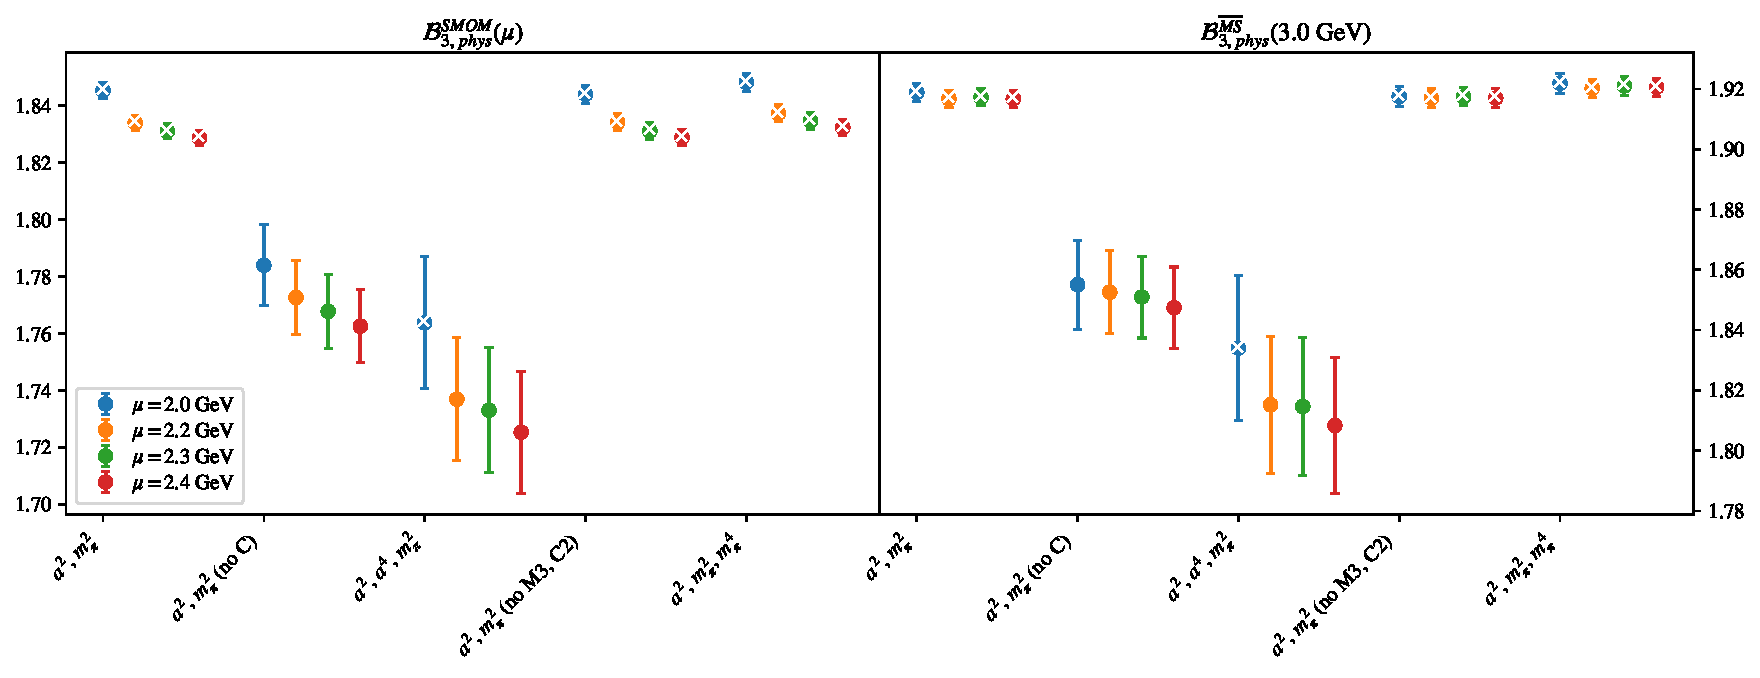
\includegraphics[page=1, width=1.1\textwidth]{SSmPP/NPR/fit_summary_bag.pdf}
\caption{$\mathcal{B}_{3}$\\(left) $\mathcal{B}_{phys}$ in RI/SMOM scheme from fit variations (fits with $p$-value $<0.05$ marked with ``$\times$"). \\(right) $\mathcal{B}_{phys}$ in $\overline{MS}$ computed using $\mathcal{B}^{\overline{MS}} = R^{\overline{MS}\leftarrow SMOM}(3.0)\sigma_{npt}(3.0,\mu) \mathcal{B}^{SMOM}(\mu)$.}
\end{figure}
\clearpage
\begin{figure}
\centering
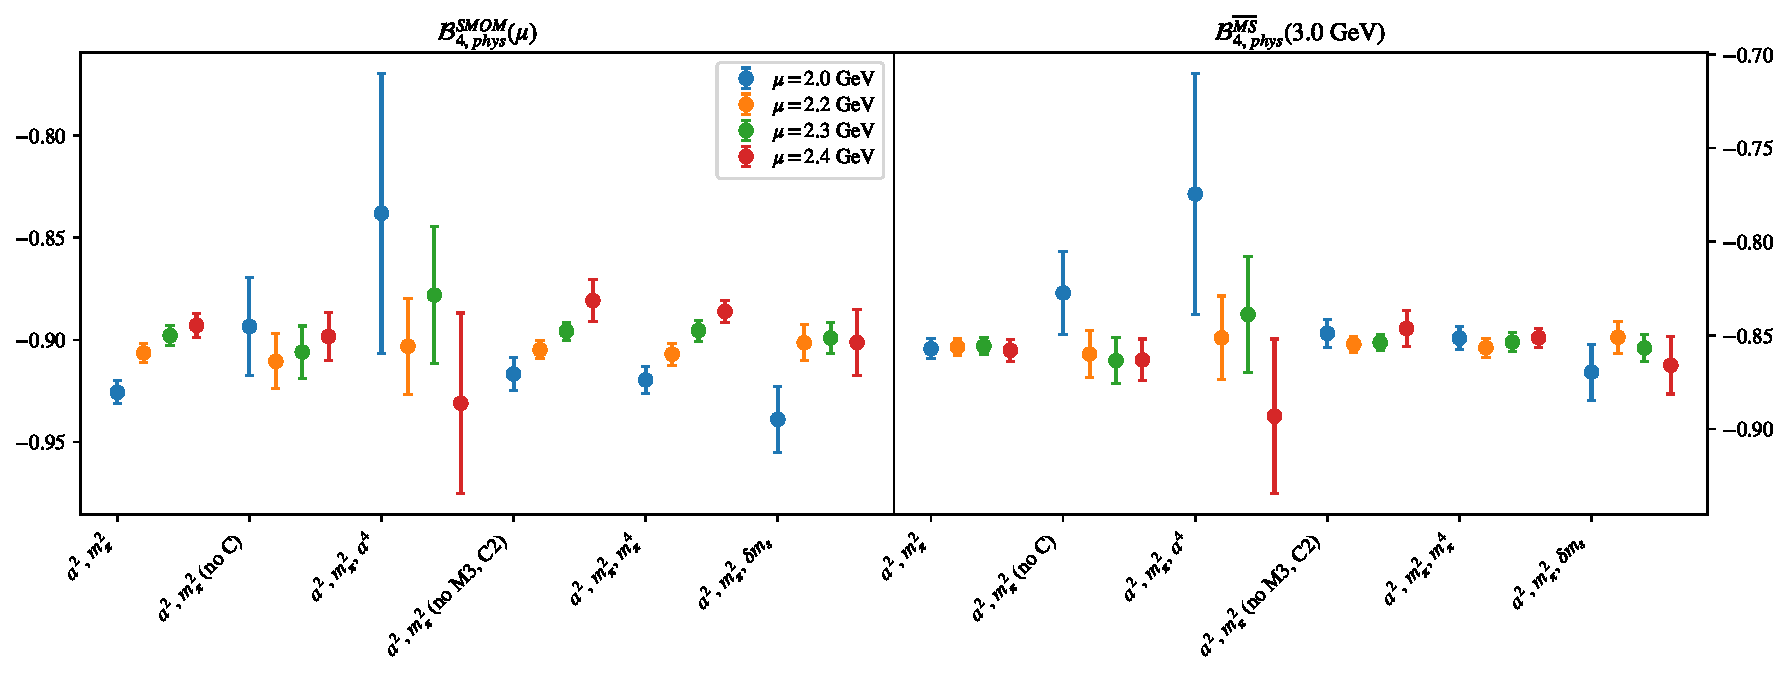
\includegraphics[page=1, width=1.1\textwidth]{SSpPP/NPR/fit_summary_bag.pdf}
\caption{$\mathcal{B}_{4}$\\(left) $\mathcal{B}_{phys}$ in RI/SMOM scheme from fit variations (fits with $p$-value $<0.05$ marked with ``$\times$"). \\(right) $\mathcal{B}_{phys}$ in $\overline{MS}$ computed using $\mathcal{B}^{\overline{MS}} = R^{\overline{MS}\leftarrow SMOM}(3.0)\sigma_{npt}(3.0,\mu) \mathcal{B}^{SMOM}(\mu)$.}
\end{figure}
\clearpage
\begin{figure}
\centering
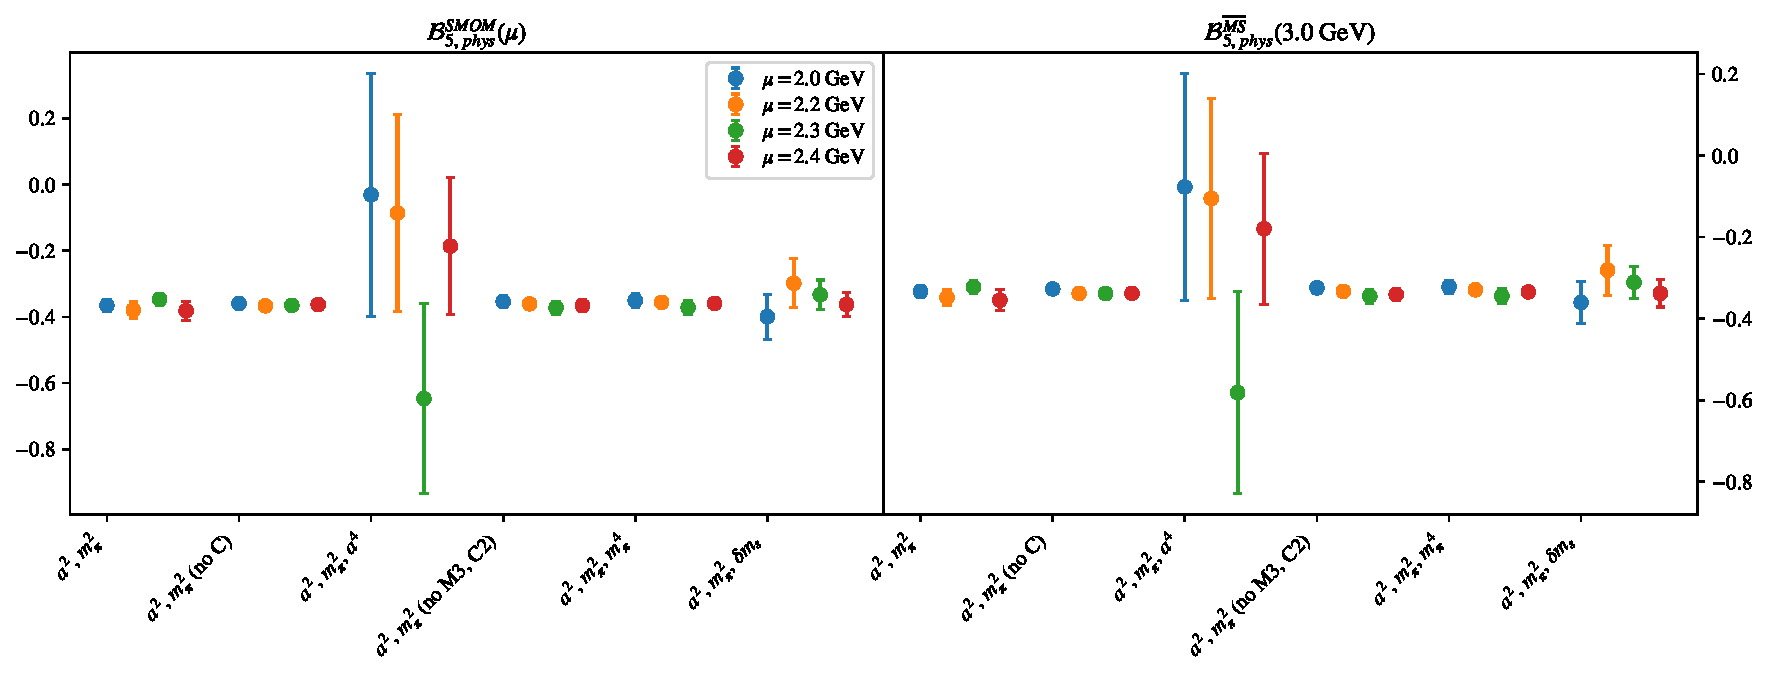
\includegraphics[page=1, width=1.1\textwidth]{TT/NPR/fit_summary_bag.pdf}
\caption{$\mathcal{B}_{5}$\\(left) $\mathcal{B}_{phys}$ in RI/SMOM scheme from fit variations (fits with $p$-value $<0.05$ marked with ``$\times$"). \\(right) $\mathcal{B}_{phys}$ in $\overline{MS}$ computed using $\mathcal{B}^{\overline{MS}} = R^{\overline{MS}\leftarrow SMOM}(3.0)\sigma_{npt}(3.0,\mu) \mathcal{B}^{SMOM}(\mu)$.}
\end{figure}
\clearpage
\section{$\mathcal{B}_1$}
\begin{table}[h!]
\begin{center}
\begin{tabular}{|c|c|c|c|c|c|c|}
\hline
$\mu$ (GeV) & $a^2$, $m_\pi^2$& $a^2$, $m_\pi^2$ (no C)& $a^2$, $m_\pi^2$, $a^4$& $a^2$, $m_\pi^2$ (no M3, C2)& $a^2$, $m_\pi^2$, $m_\pi^4$& $a^2$, $m_\pi^2$, $\delta m_s$\\
\hline
2.0& \hyperlink{VVpAA/NPR/bag_a2m2_20.pdf.1}{\textbf{1.4024(29)}: 2.347 (0.039)} & \hyperlink{VVpAA/NPR/bag_a2m2noC_20.pdf.1}{\textbf{1.436(12)}: 0.223 (0.8)} & \hyperlink{VVpAA/NPR/bag_a2a4m2_20.pdf.1}{\textbf{1.457(21)}: 1.329 (0.256)} & \hyperlink{VVpAA/NPR/bag_a2m2mcut_20.pdf.1}{\textbf{1.4062(33)}: 2.004 (0.111)} & \hyperlink{VVpAA/NPR/bag_a2m2m4_20.pdf.1}{\textbf{1.4051(33)}: 2.362 (0.051)} & \hyperlink{VVpAA/NPR/bag_a2m2delm_20.pdf.1}{\textbf{1.4029(29)}: 0.738 (0.566)}\\
2.2& \hyperlink{VVpAA/NPR/bag_a2m2_22.pdf.1}{\textbf{1.3949(29)}: 2.793 (0.016)} & \hyperlink{VVpAA/NPR/bag_a2m2noC_22.pdf.1}{\textbf{1.431(12)}: 0.353 (0.703)} & \hyperlink{VVpAA/NPR/bag_a2a4m2_22.pdf.1}{\textbf{1.453(21)}: 1.664 (0.155)} & \hyperlink{VVpAA/NPR/bag_a2m2mcut_22.pdf.1}{\textbf{1.3989(32)}: 2.36 (0.069)} & \hyperlink{VVpAA/NPR/bag_a2m2m4_22.pdf.1}{\textbf{1.3978(33)}: 2.785 (0.025)} & \hyperlink{VVpAA/NPR/bag_a2m2delm_22.pdf.1}{\textbf{1.3954(29)}: 0.922 (0.45)}\\
2.3& \hyperlink{VVpAA/NPR/bag_a2m2_23.pdf.1}{\textbf{1.3916(28)}: 2.928 (0.012)} & \hyperlink{VVpAA/NPR/bag_a2m2noC_23.pdf.1}{\textbf{1.428(12)}: 0.357 (0.7)} & \hyperlink{VVpAA/NPR/bag_a2a4m2_23.pdf.1}{\textbf{1.451(21)}: 1.727 (0.141)} & \hyperlink{VVpAA/NPR/bag_a2m2mcut_23.pdf.1}{\textbf{1.3958(32)}: 2.481 (0.059)} & \hyperlink{VVpAA/NPR/bag_a2m2m4_23.pdf.1}{\textbf{1.3945(33)}: 2.854 (0.022)} & \hyperlink{VVpAA/NPR/bag_a2m2delm_23.pdf.1}{\textbf{1.3921(29)}: 0.949 (0.434)}\\
2.4& \hyperlink{VVpAA/NPR/bag_a2m2_24.pdf.1}{\textbf{1.3887(28)}: 2.989 (0.011)} & \hyperlink{VVpAA/NPR/bag_a2m2noC_24.pdf.1}{\textbf{1.425(12)}: 0.371 (0.69)} & \hyperlink{VVpAA/NPR/bag_a2a4m2_24.pdf.1}{\textbf{1.448(21)}: 1.801 (0.126)} & \hyperlink{VVpAA/NPR/bag_a2m2mcut_24.pdf.1}{\textbf{1.3929(32)}: 2.515 (0.056)} & \hyperlink{VVpAA/NPR/bag_a2m2m4_24.pdf.1}{\textbf{1.3918(33)}: 2.957 (0.019)} & \hyperlink{VVpAA/NPR/bag_a2m2delm_24.pdf.1}{\textbf{1.3892(29)}: 0.985 (0.414)}\\
\hline
\end{tabular}
\caption{Physical point value from chiral and continuum extrapolation at renormalisation scale $\mu$. Entries are \textbf{value(error)}: $\chi^2/\text{DOF}$ ($p$-value).}
\end{center}
\end{table}
\begin{table}[h!]
\begin{center}
\begin{tabular}{|c c|c|c|c|c|c|c|}
\hline
$\mu$ (GeV) &  & $a^2$, $m_\pi^2$& $a^2$, $m_\pi^2$ (no C)& $a^2$, $m_\pi^2$, $a^4$& $a^2$, $m_\pi^2$ (no M3, C2)& $a^2$, $m_\pi^2$, $m_\pi^4$& $a^2$, $m_\pi^2$, $\delta m_s$\\
\hline
\multirow{3}{0.5in}{2.0} & $\alpha$ & 0.138(10)& -0.053(73)& -0.37(19)& 0.126(11)& 0.130(11)& 0.141(10)\\
 & $\beta$ & 0.00374(21)& 0.00337(39)& 0.00403(25)& 0.00314(34)& 0.0022(10)& 0.00502(50)\\
 & $\gamma$ &  &  & 1.03(39)&  & 0.000142(92)& -0.049(16)\\
\hline
\multirow{3}{0.5in}{2.2} & $\alpha$ & 0.143(10)& -0.061(73)& -0.40(19)& 0.131(11)& 0.135(11)& 0.147(10)\\
 & $\beta$ & 0.00372(21)& 0.00330(39)& 0.00403(25)& 0.00307(33)& 0.0020(10)& 0.00510(51)\\
 & $\gamma$ &  &  & 1.10(39)&  & 0.000158(92)& -0.054(17)\\
\hline
\multirow{3}{0.5in}{2.3} & $\alpha$ & 0.145(10)& -0.064(73)& -0.40(19)& 0.132(11)& 0.137(11)& 0.148(10)\\
 & $\beta$ & 0.00372(21)& 0.00330(39)& 0.00404(25)& 0.00306(33)& 0.0019(10)& 0.00513(51)\\
 & $\gamma$ &  &  & 1.12(39)&  & 0.000160(91)& -0.054(17)\\
\hline
\multirow{3}{0.5in}{2.4} & $\alpha$ & 0.146(10)& -0.064(73)& -0.40(19)& 0.133(11)& 0.137(11)& 0.149(10)\\
 & $\beta$ & 0.00373(21)& 0.00329(39)& 0.00405(25)& 0.00306(33)& 0.0019(10)& 0.00515(51)\\
 & $\gamma$ &  &  & 1.12(39)&  & 0.000162(91)& -0.055(17)\\
\hline
\end{tabular}
\caption{Fit values of coefficients in $Q = Q_{phys} + \mathbf{\alpha} a^2 + \mathbf{\beta}\left(\frac{m_\pi^2}{f_\pi^2}-\frac{m_{\pi,PDG}^2}{f_\pi^2}\right) + \gamma(\ldots)$}
\end{center}
\end{table}
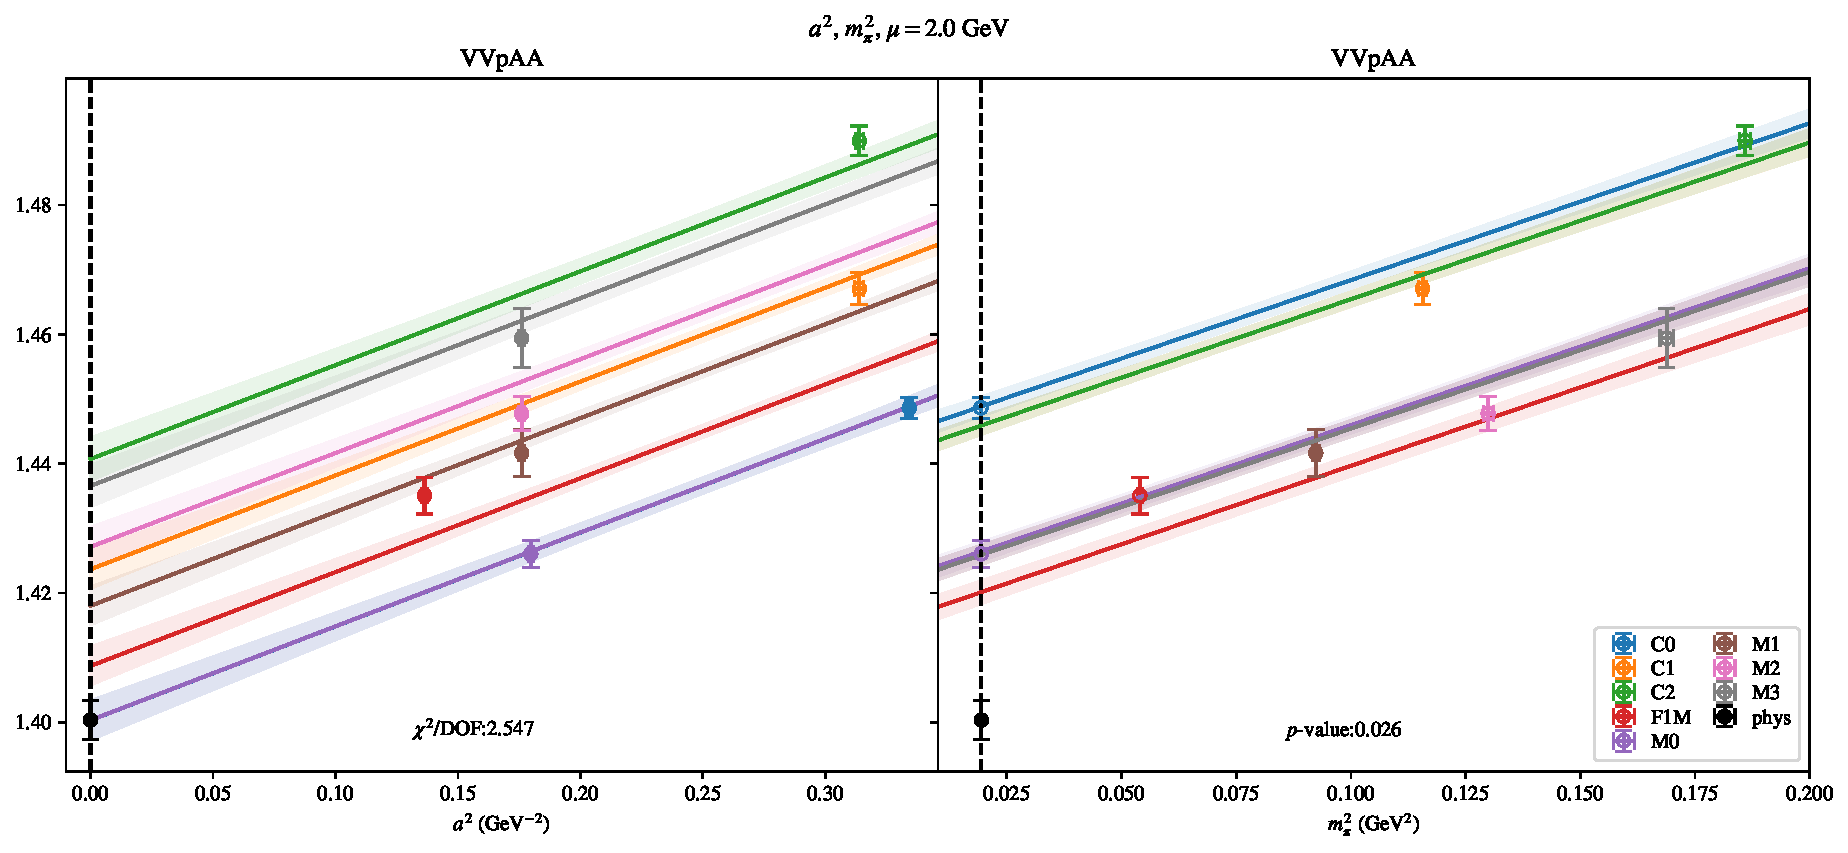
\includepdf[link, pages=-]{VVpAA/NPR/bag_a2m2_20.pdf}
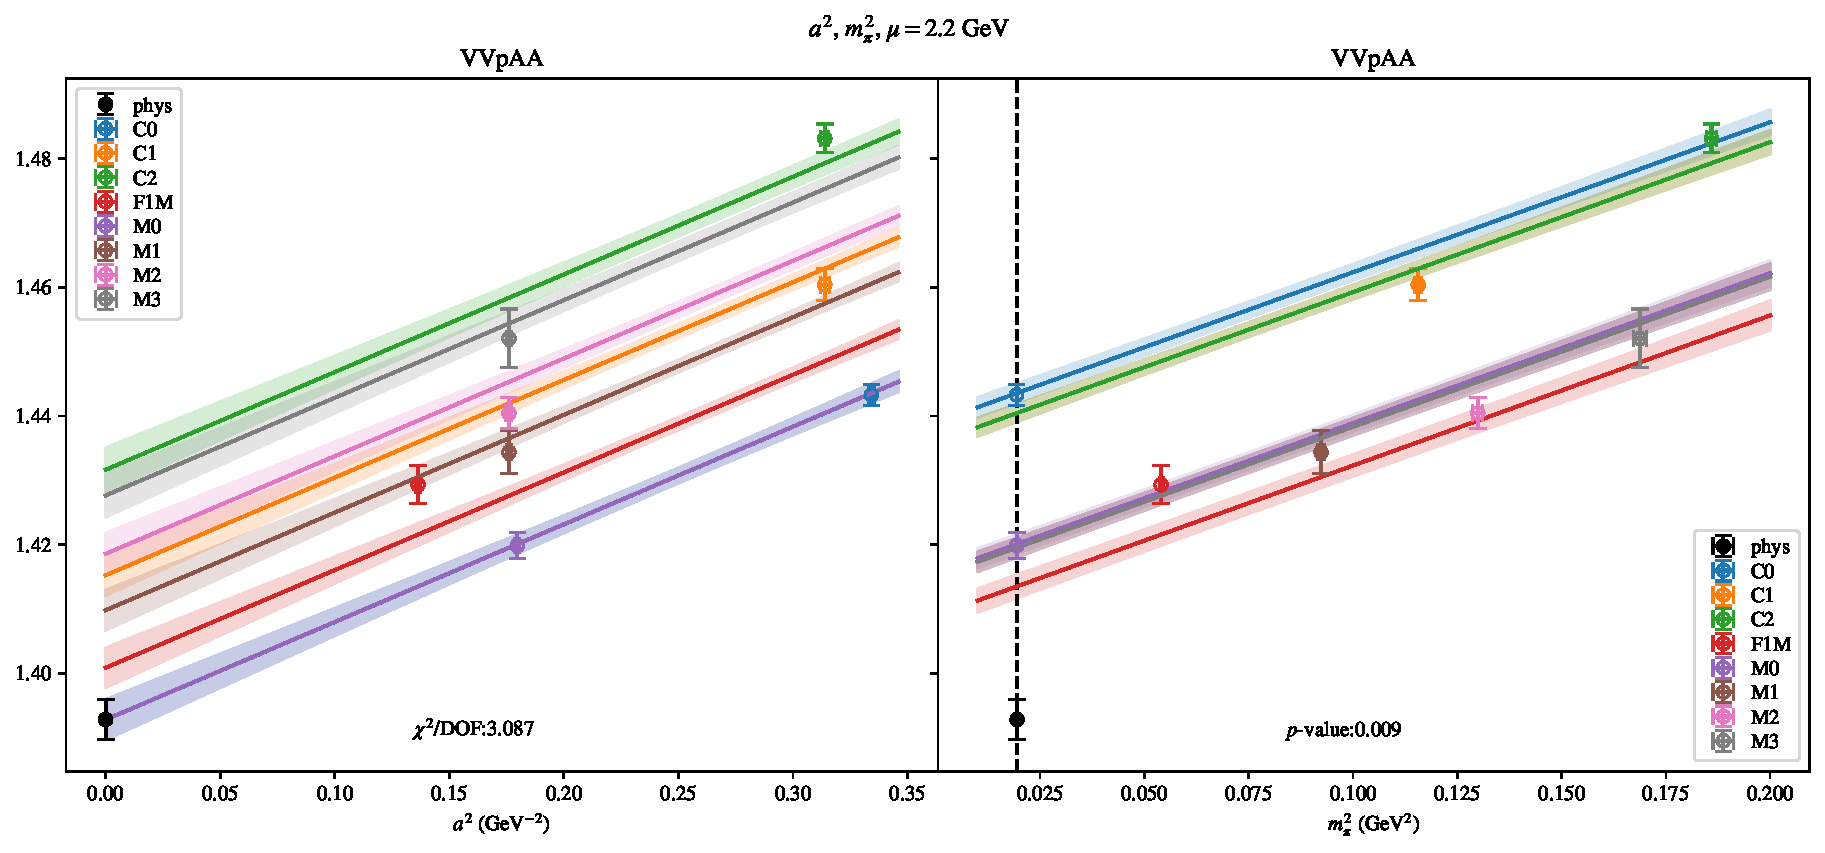
\includepdf[link, pages=-]{VVpAA/NPR/bag_a2m2_22.pdf}
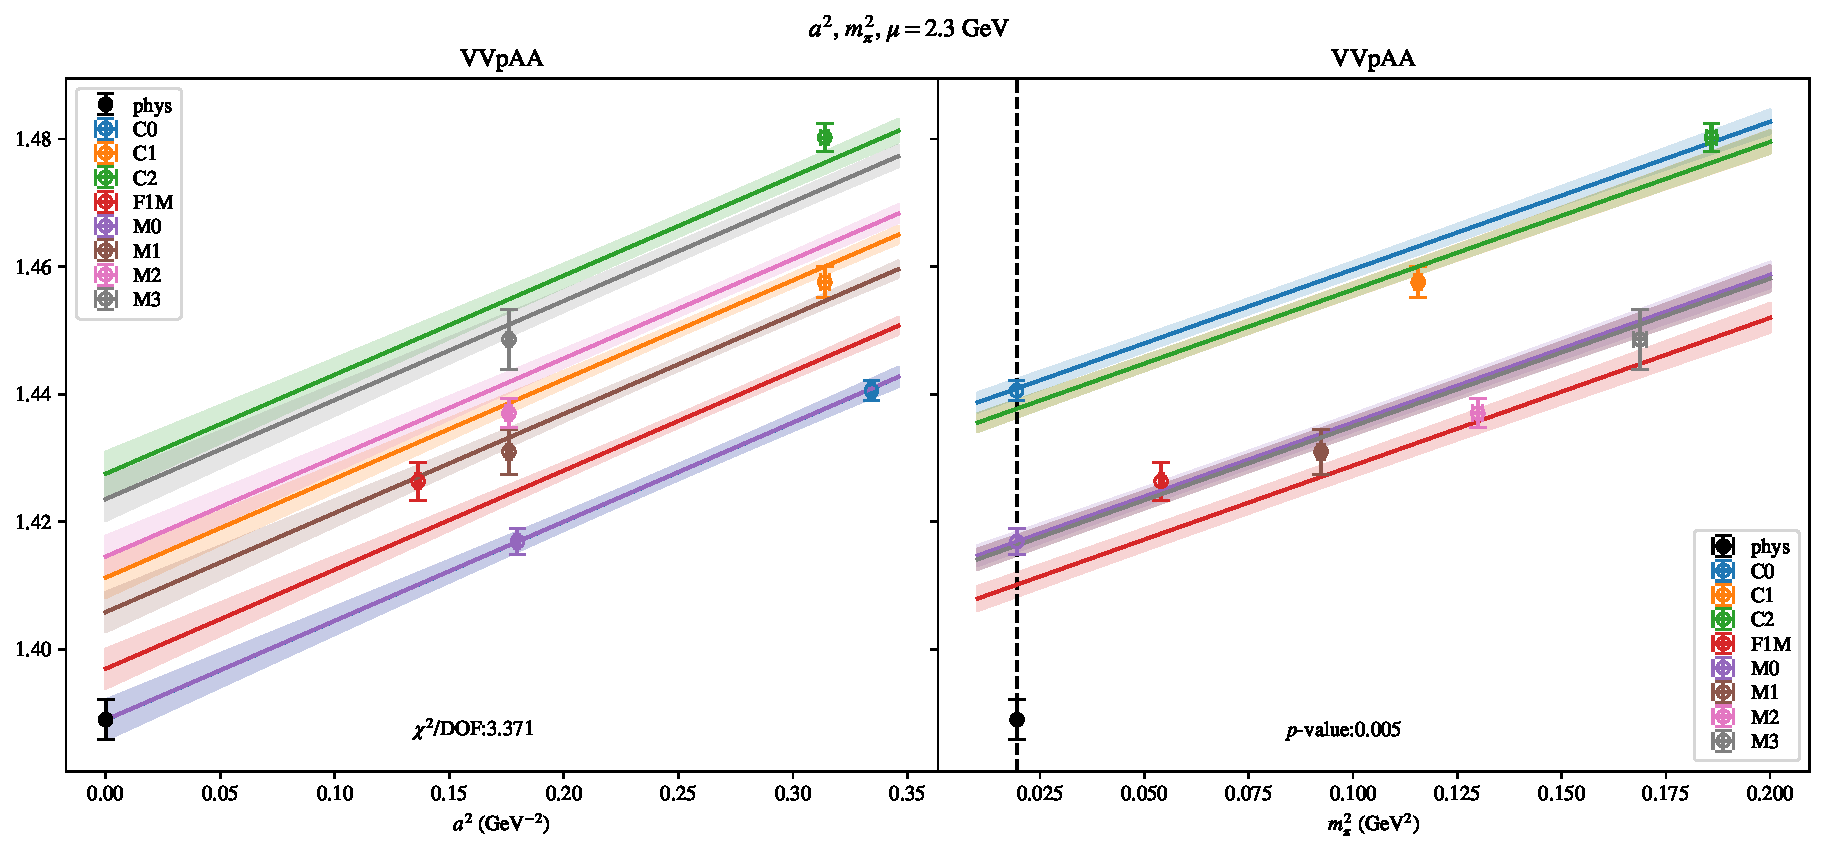
\includepdf[link, pages=-]{VVpAA/NPR/bag_a2m2_23.pdf}
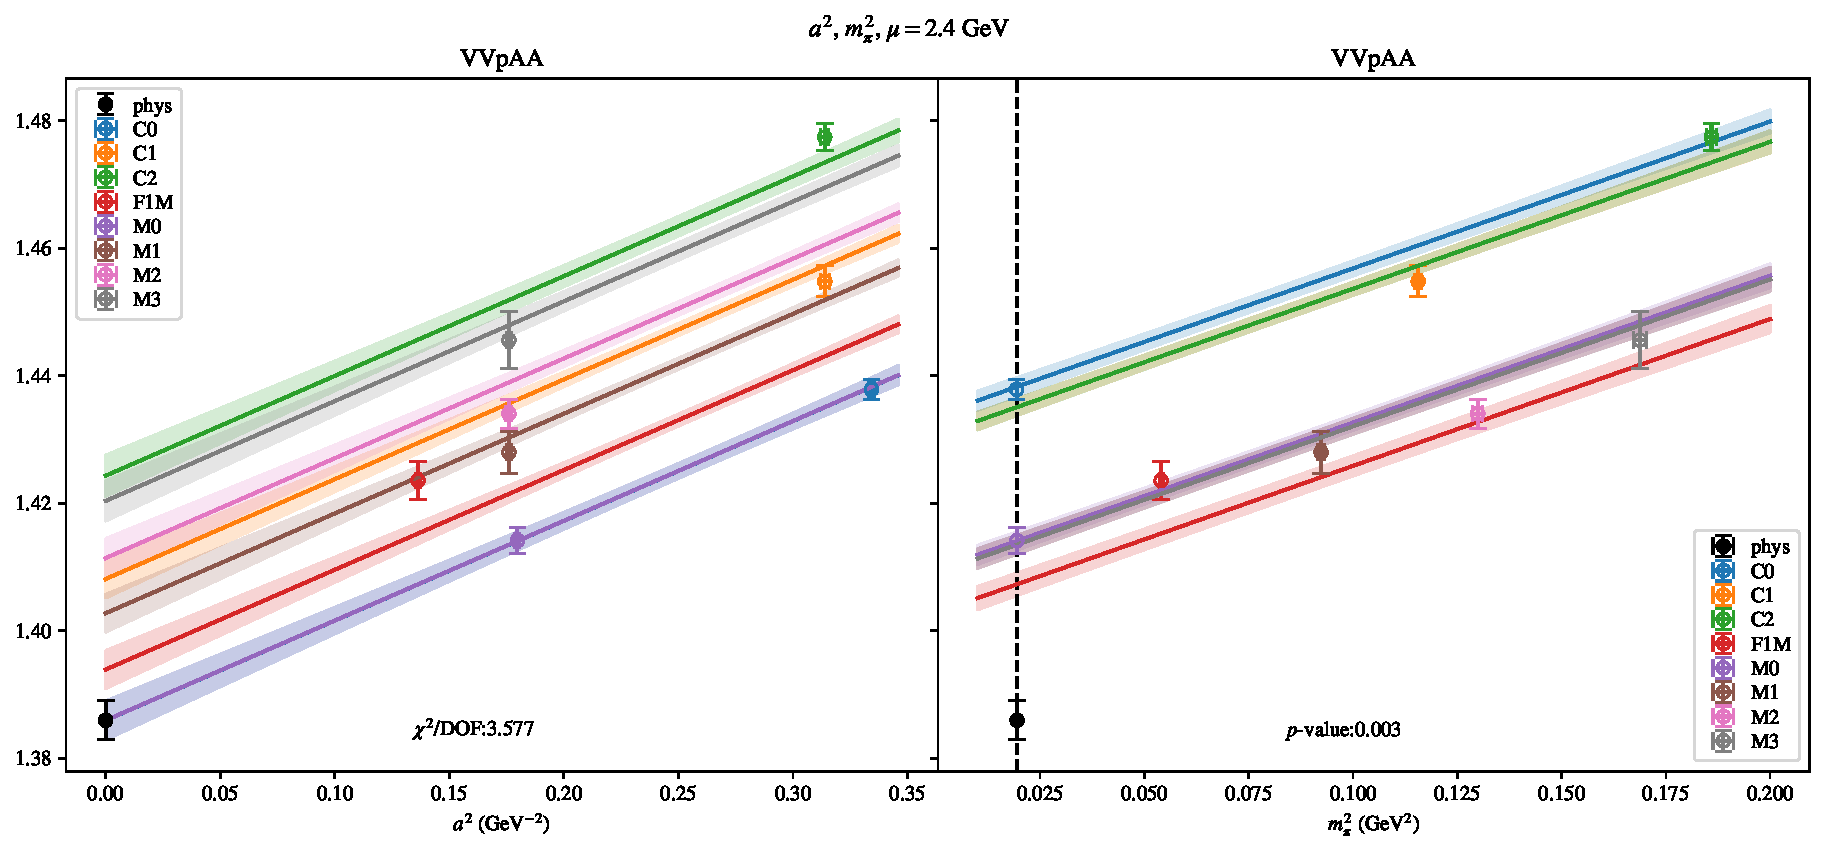
\includepdf[link, pages=-]{VVpAA/NPR/bag_a2m2_24.pdf}
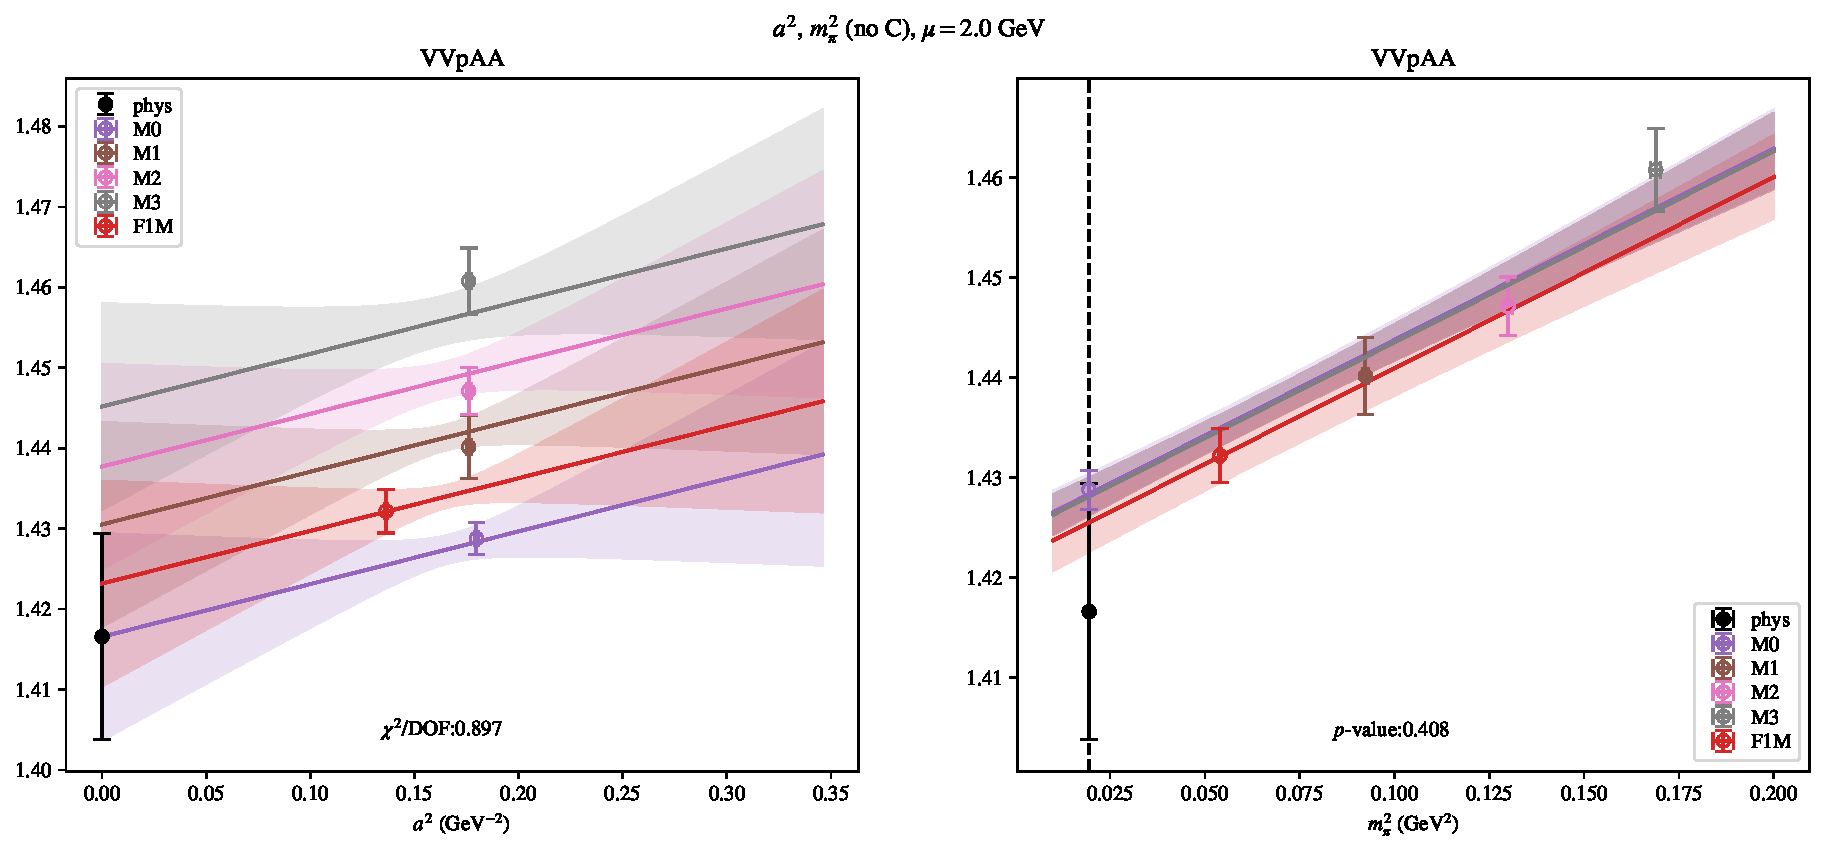
\includepdf[link, pages=-]{VVpAA/NPR/bag_a2m2noC_20.pdf}
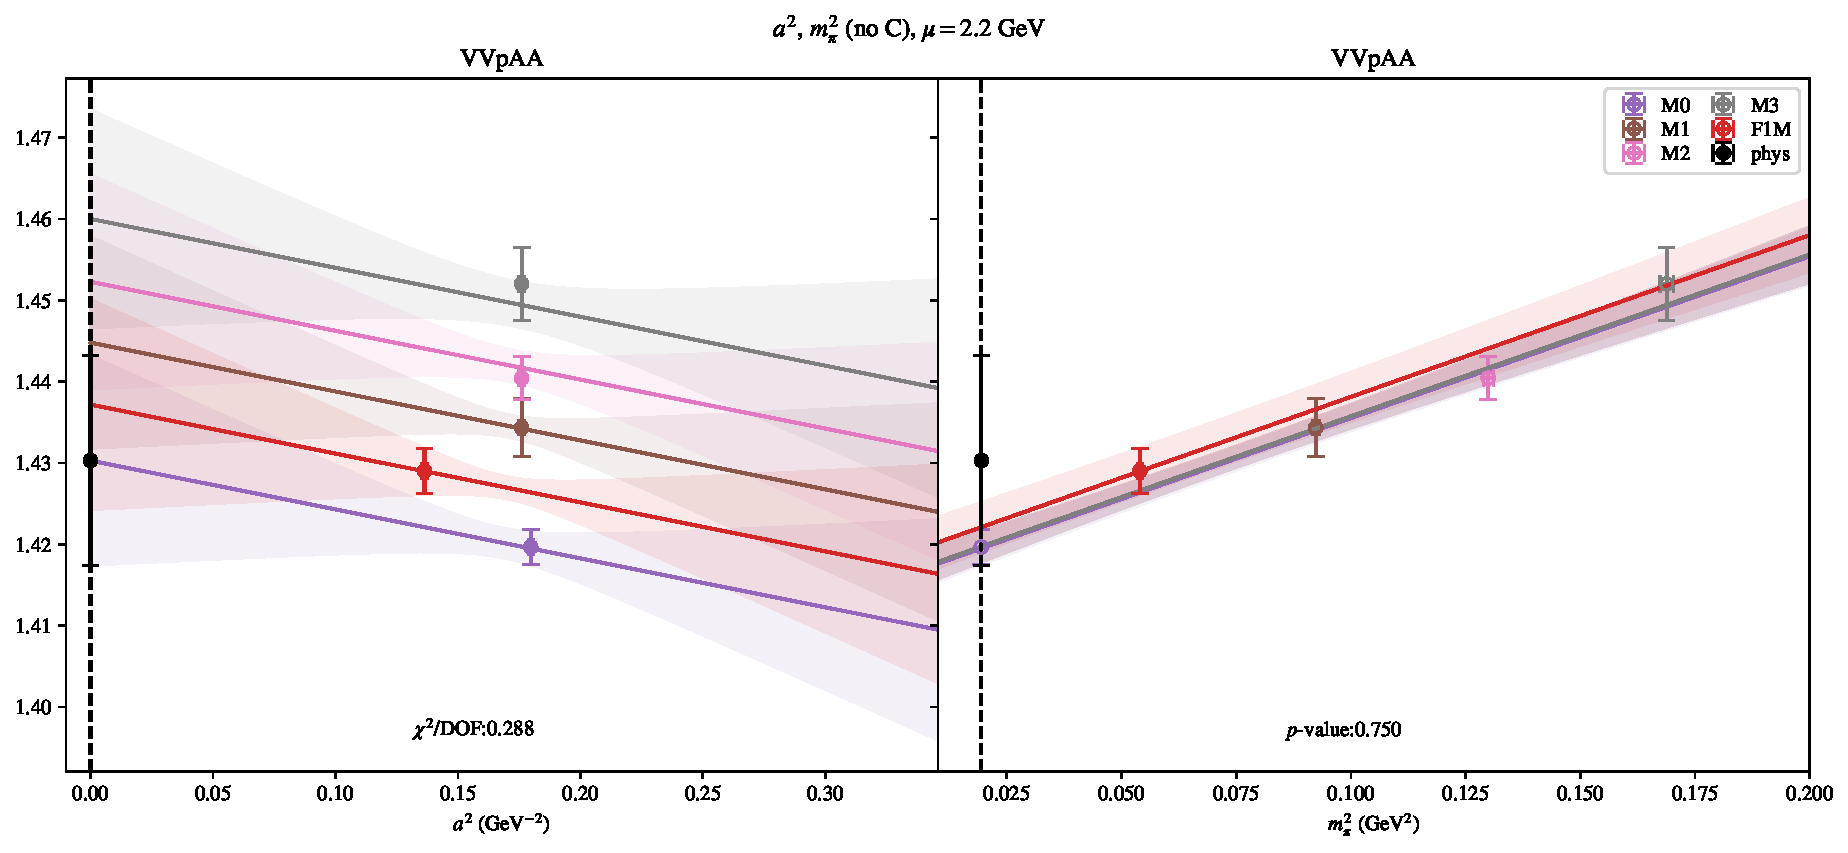
\includepdf[link, pages=-]{VVpAA/NPR/bag_a2m2noC_22.pdf}
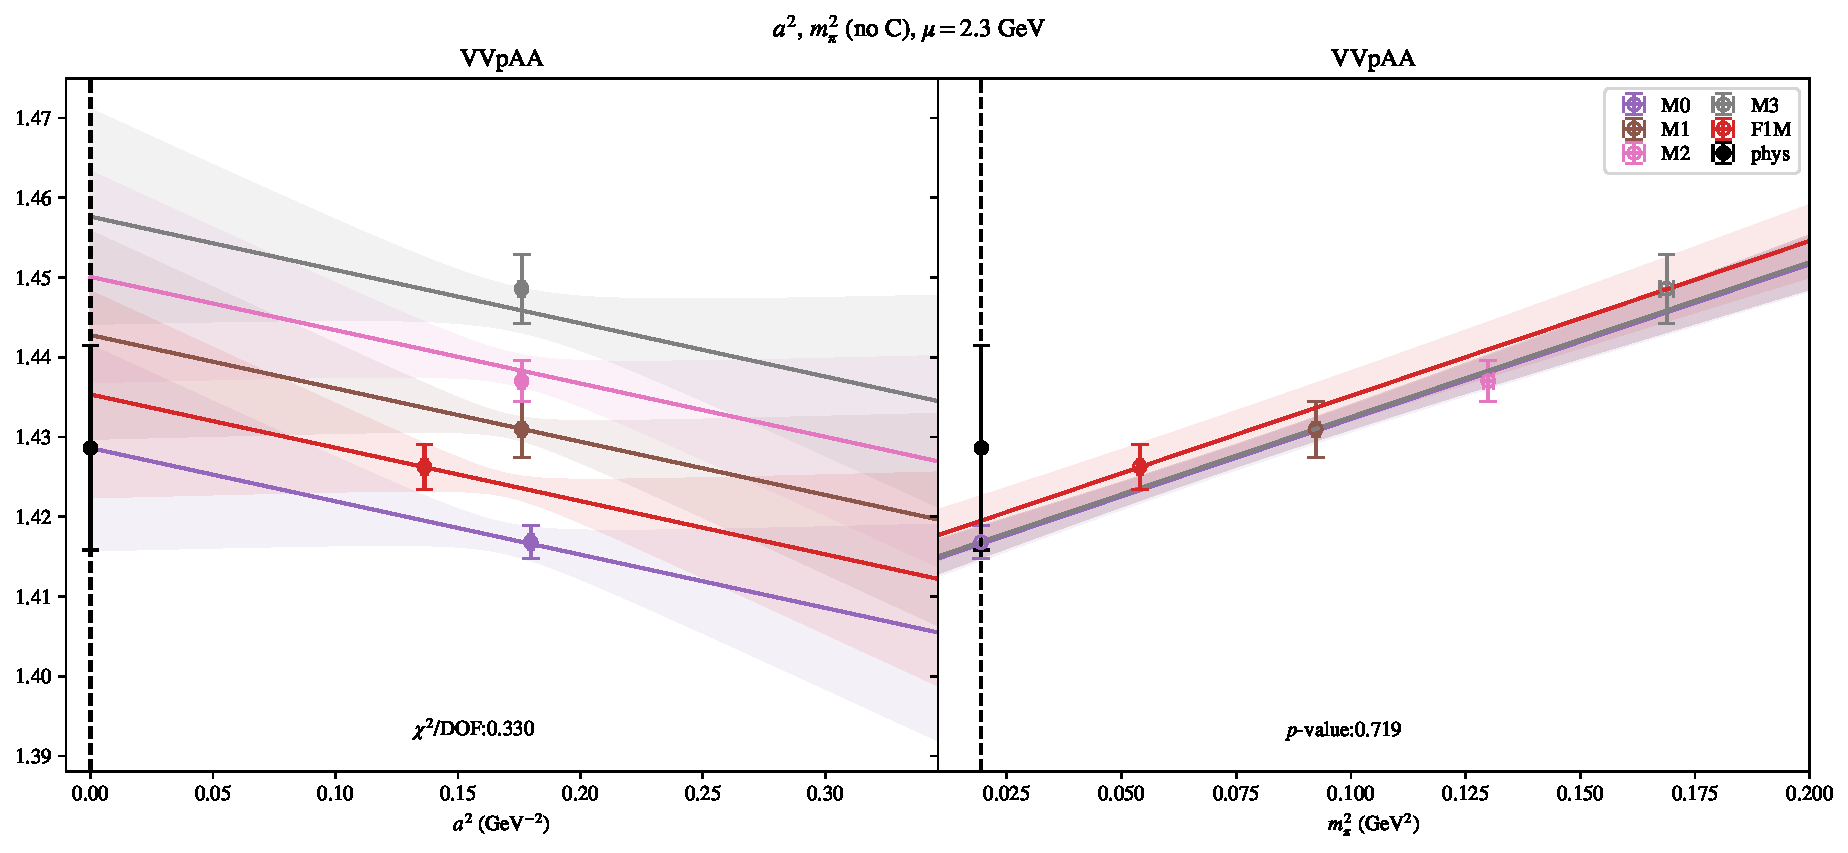
\includepdf[link, pages=-]{VVpAA/NPR/bag_a2m2noC_23.pdf}
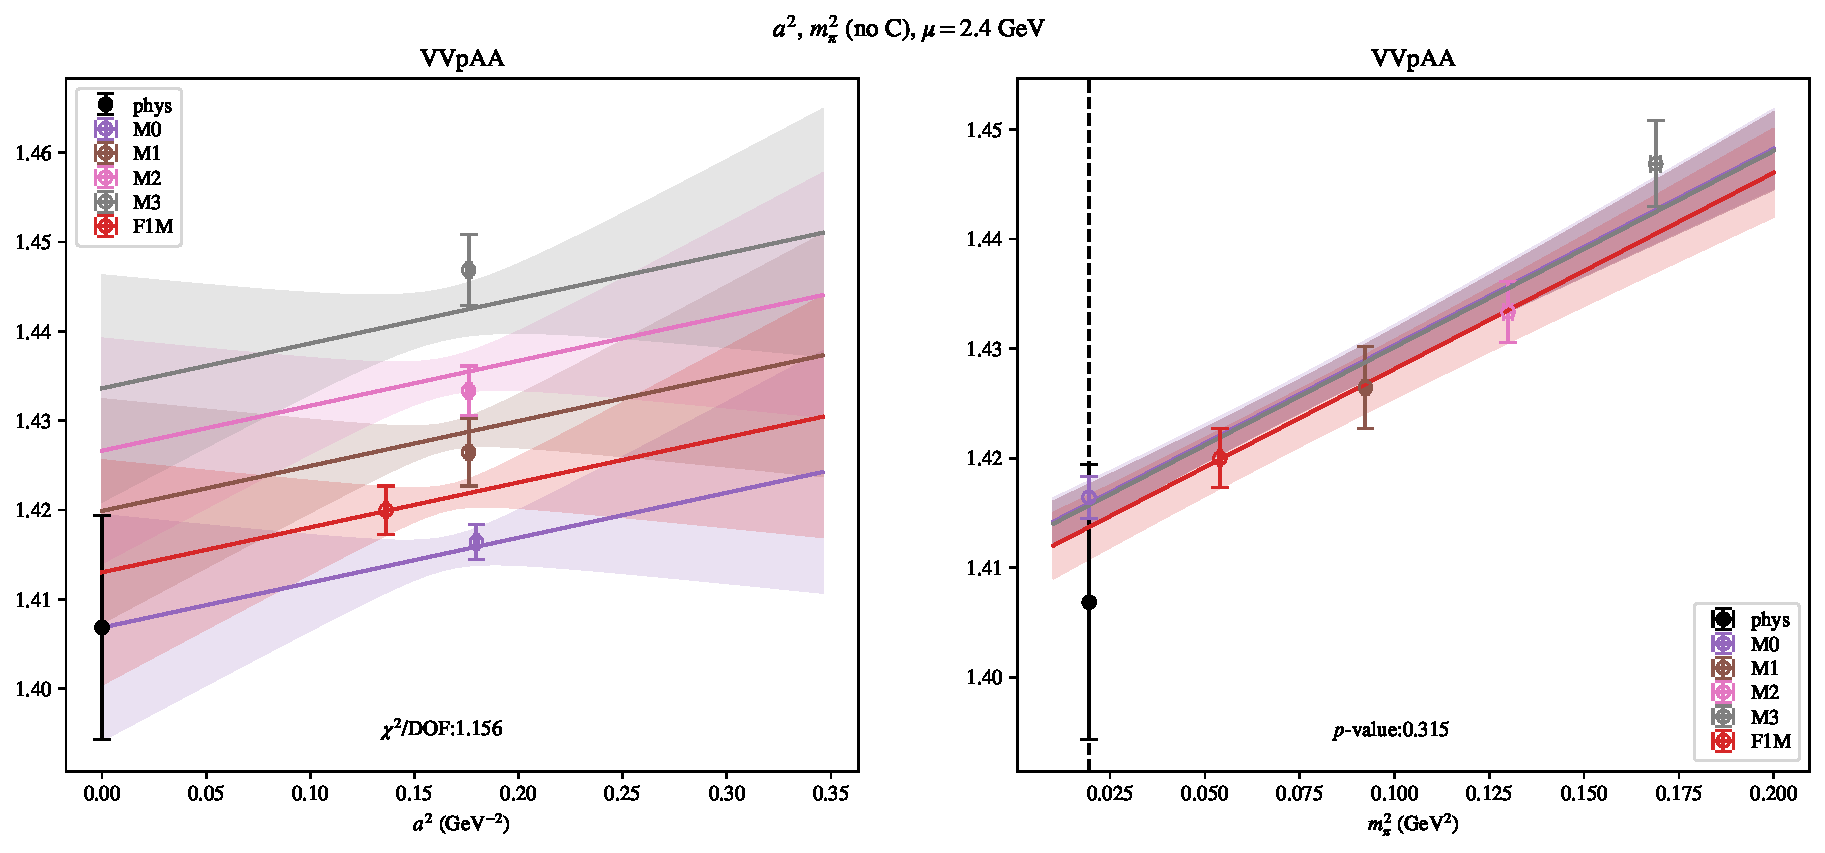
\includepdf[link, pages=-]{VVpAA/NPR/bag_a2m2noC_24.pdf}
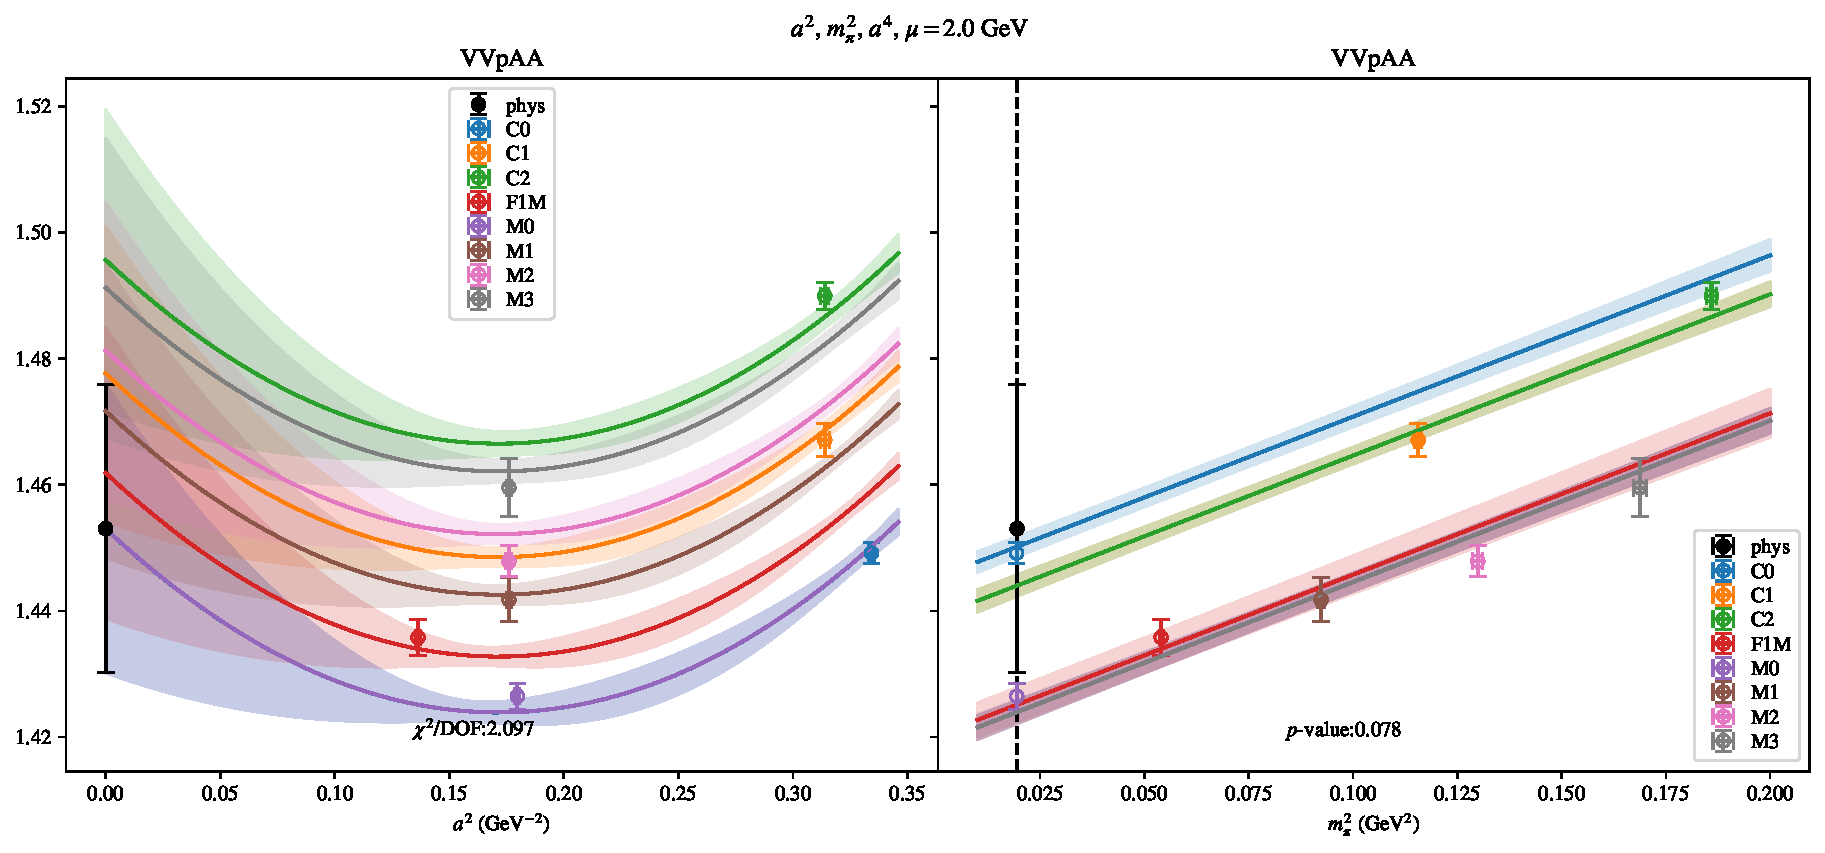
\includepdf[link, pages=-]{VVpAA/NPR/bag_a2a4m2_20.pdf}
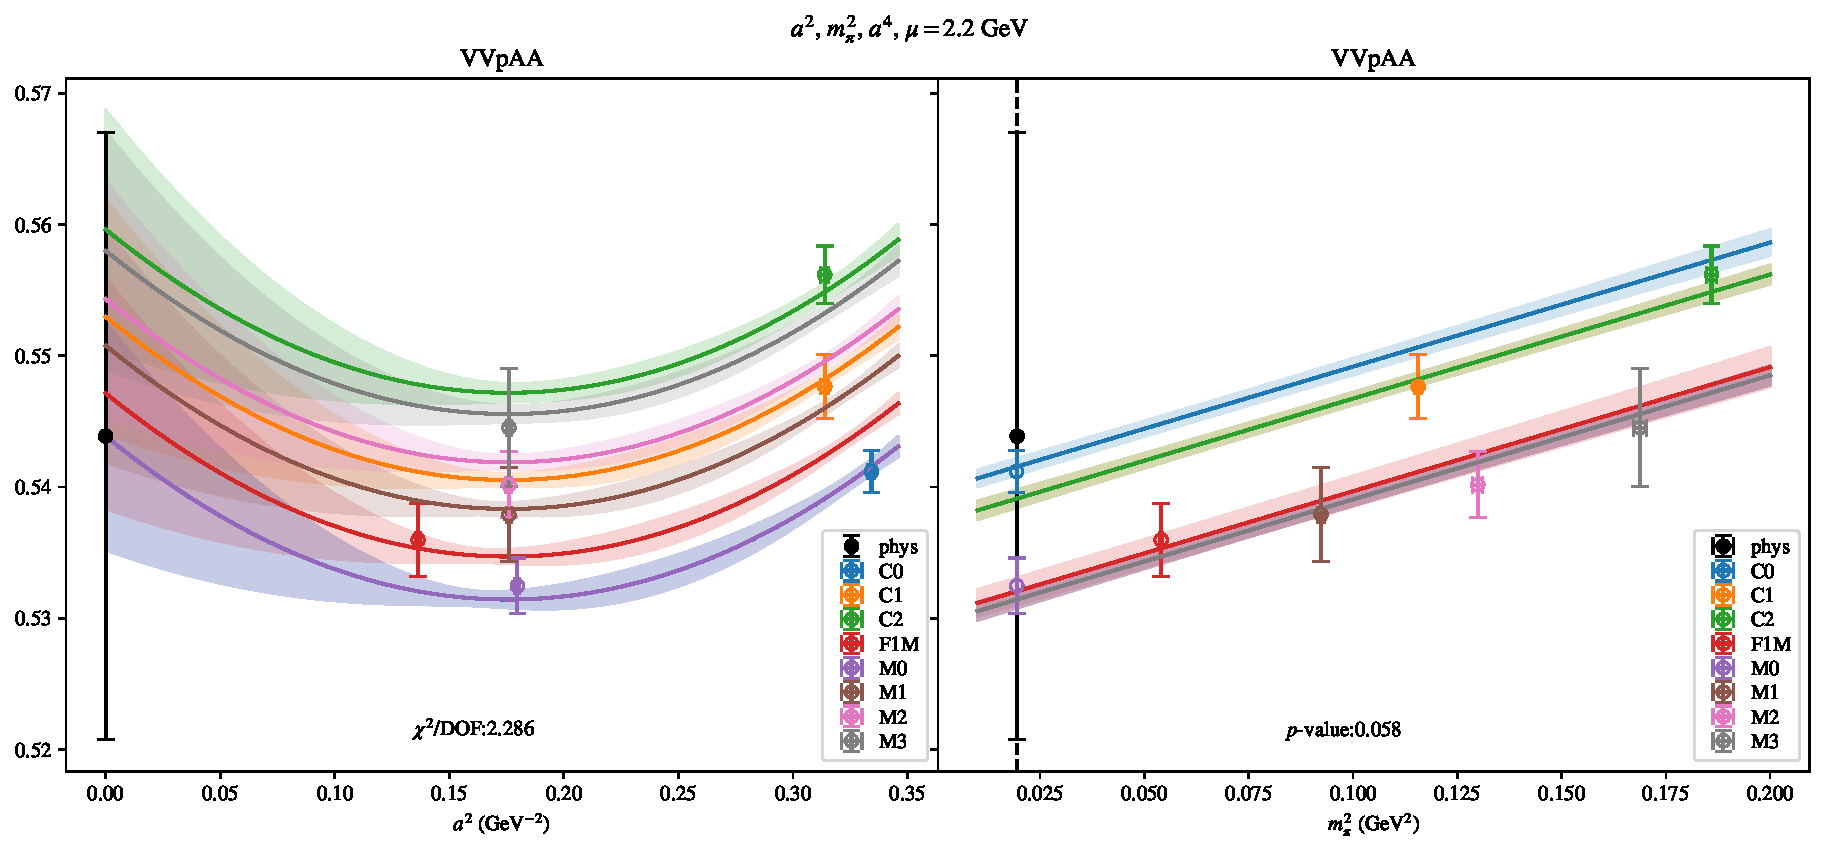
\includepdf[link, pages=-]{VVpAA/NPR/bag_a2a4m2_22.pdf}
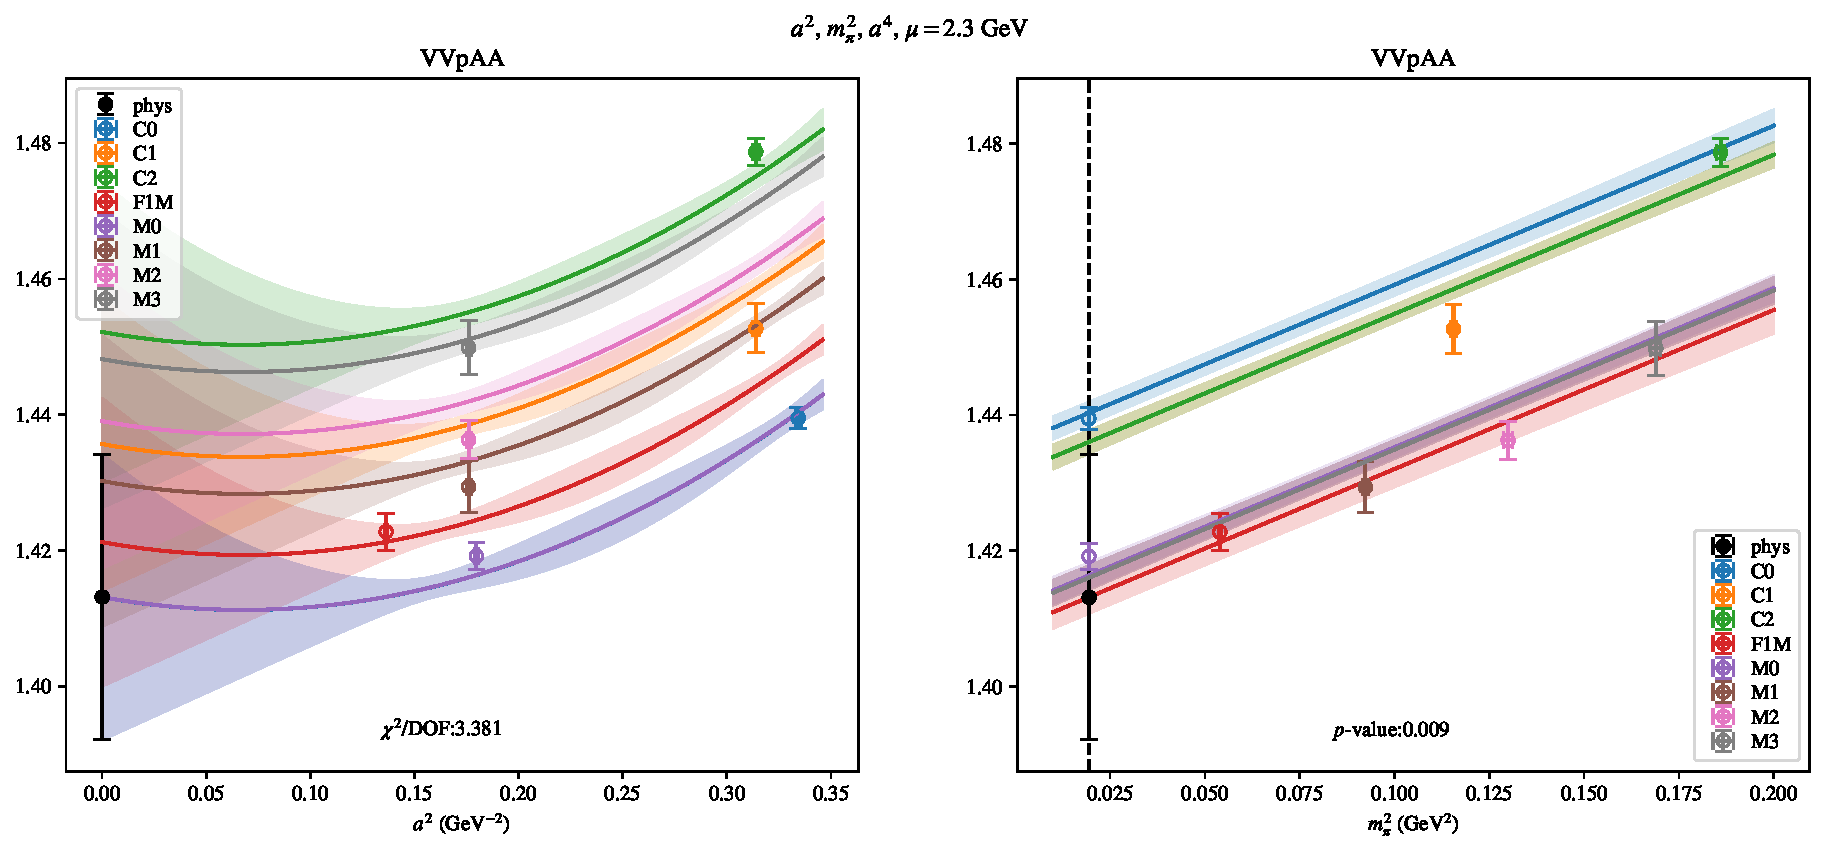
\includepdf[link, pages=-]{VVpAA/NPR/bag_a2a4m2_23.pdf}
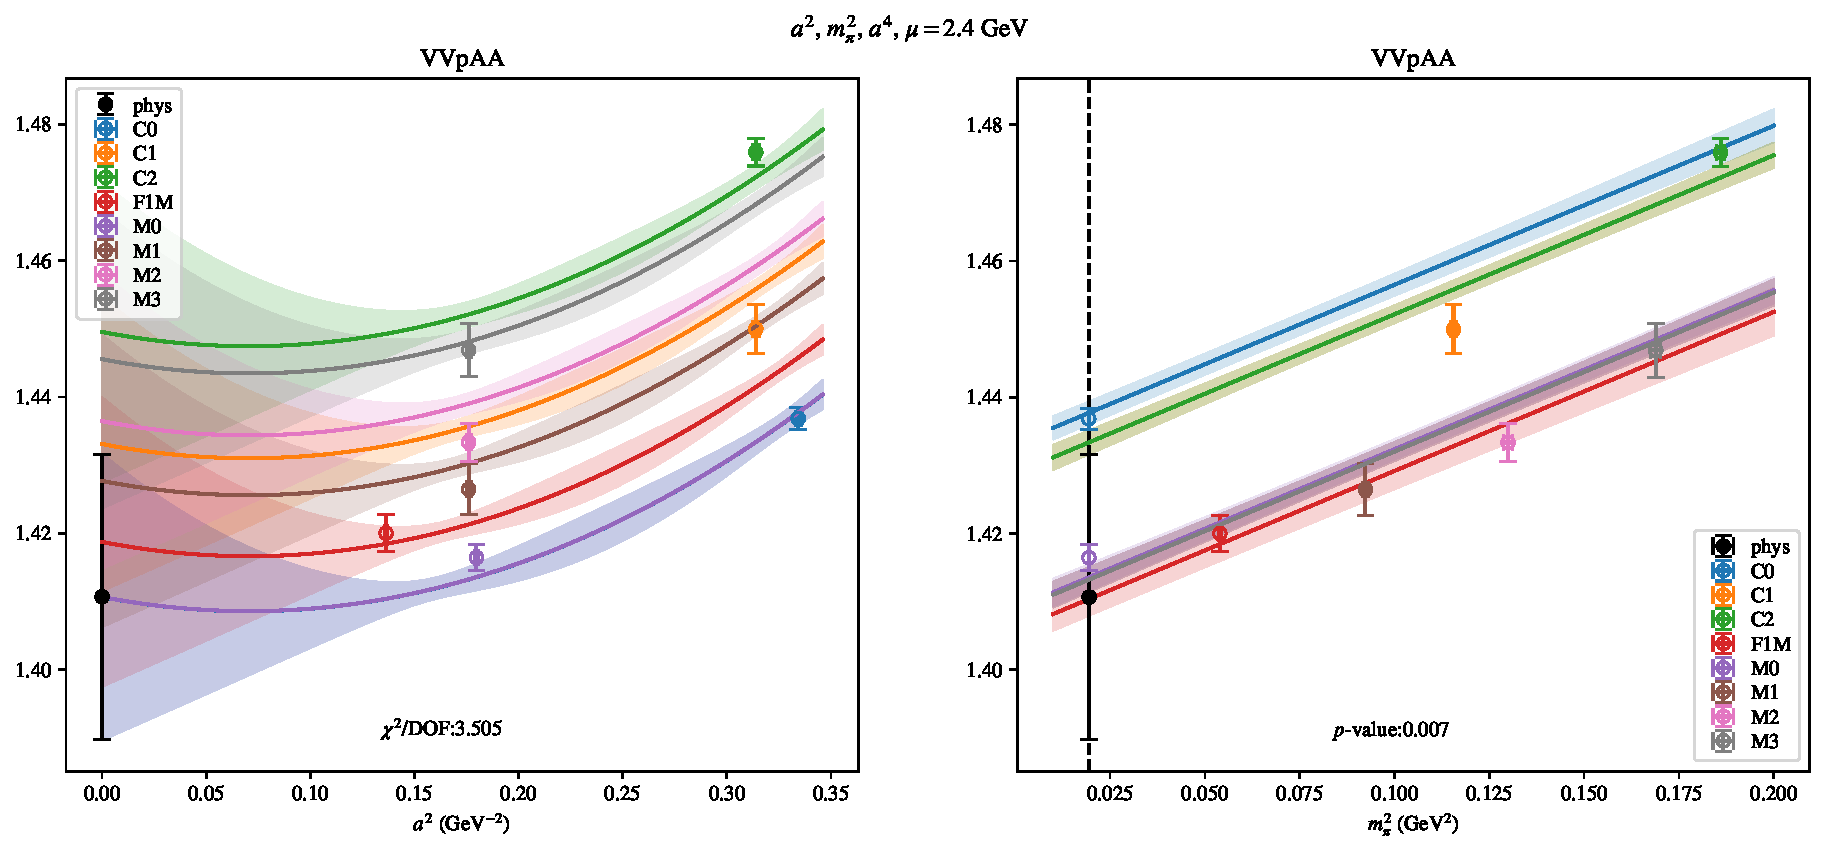
\includepdf[link, pages=-]{VVpAA/NPR/bag_a2a4m2_24.pdf}
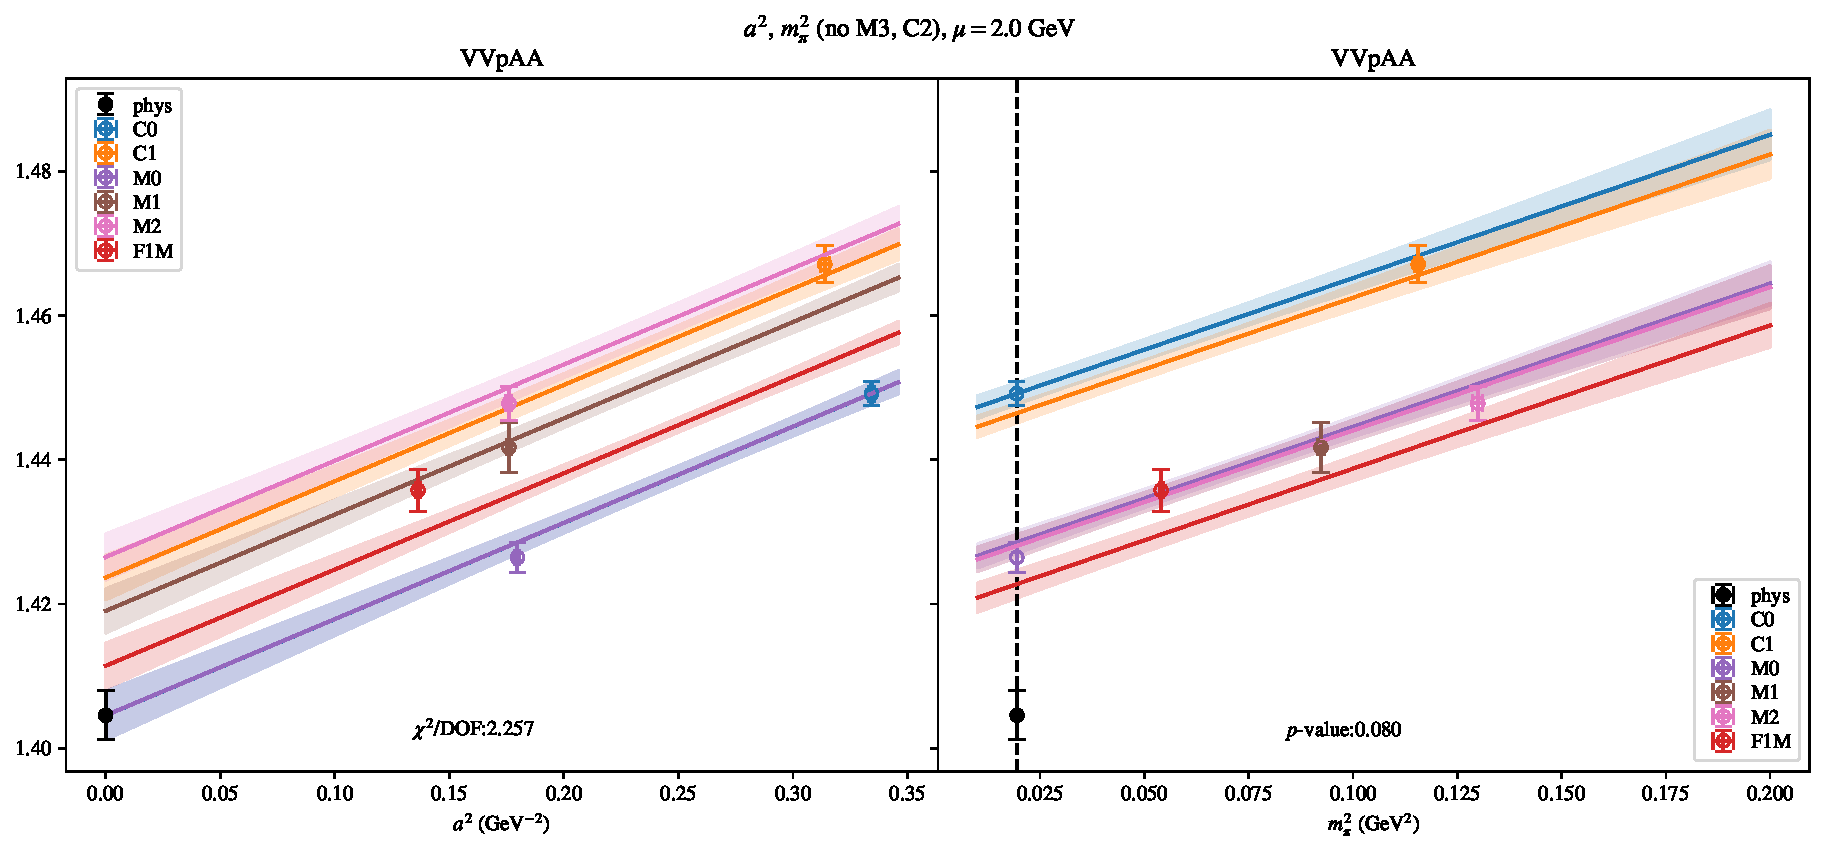
\includepdf[link, pages=-]{VVpAA/NPR/bag_a2m2mcut_20.pdf}
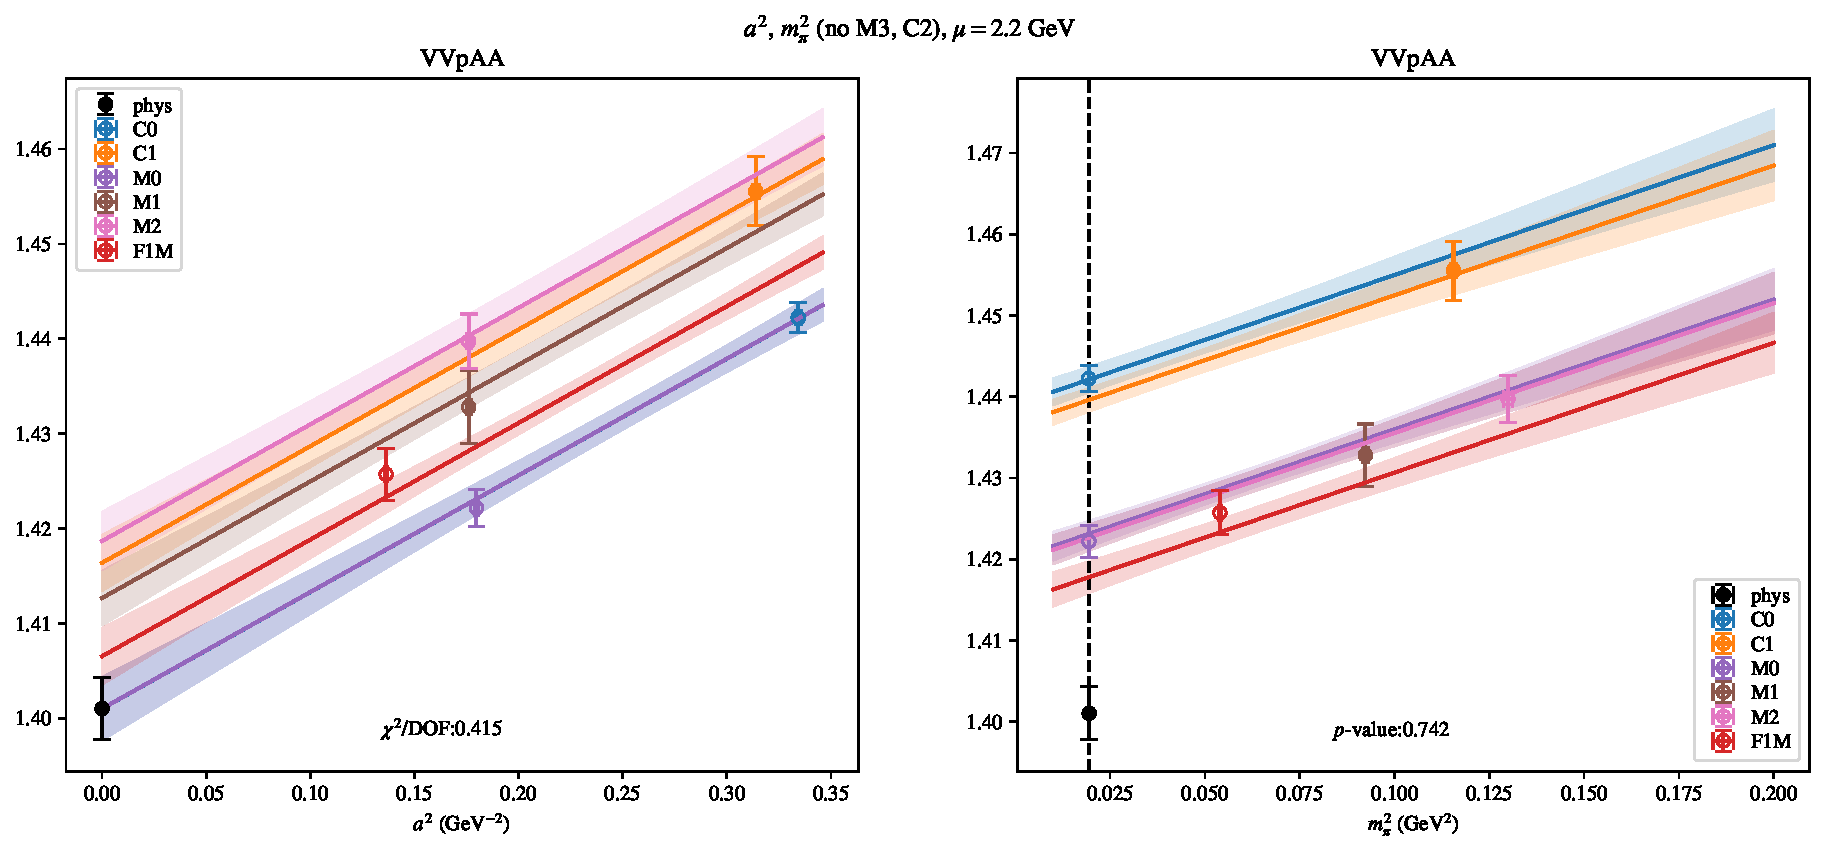
\includepdf[link, pages=-]{VVpAA/NPR/bag_a2m2mcut_22.pdf}
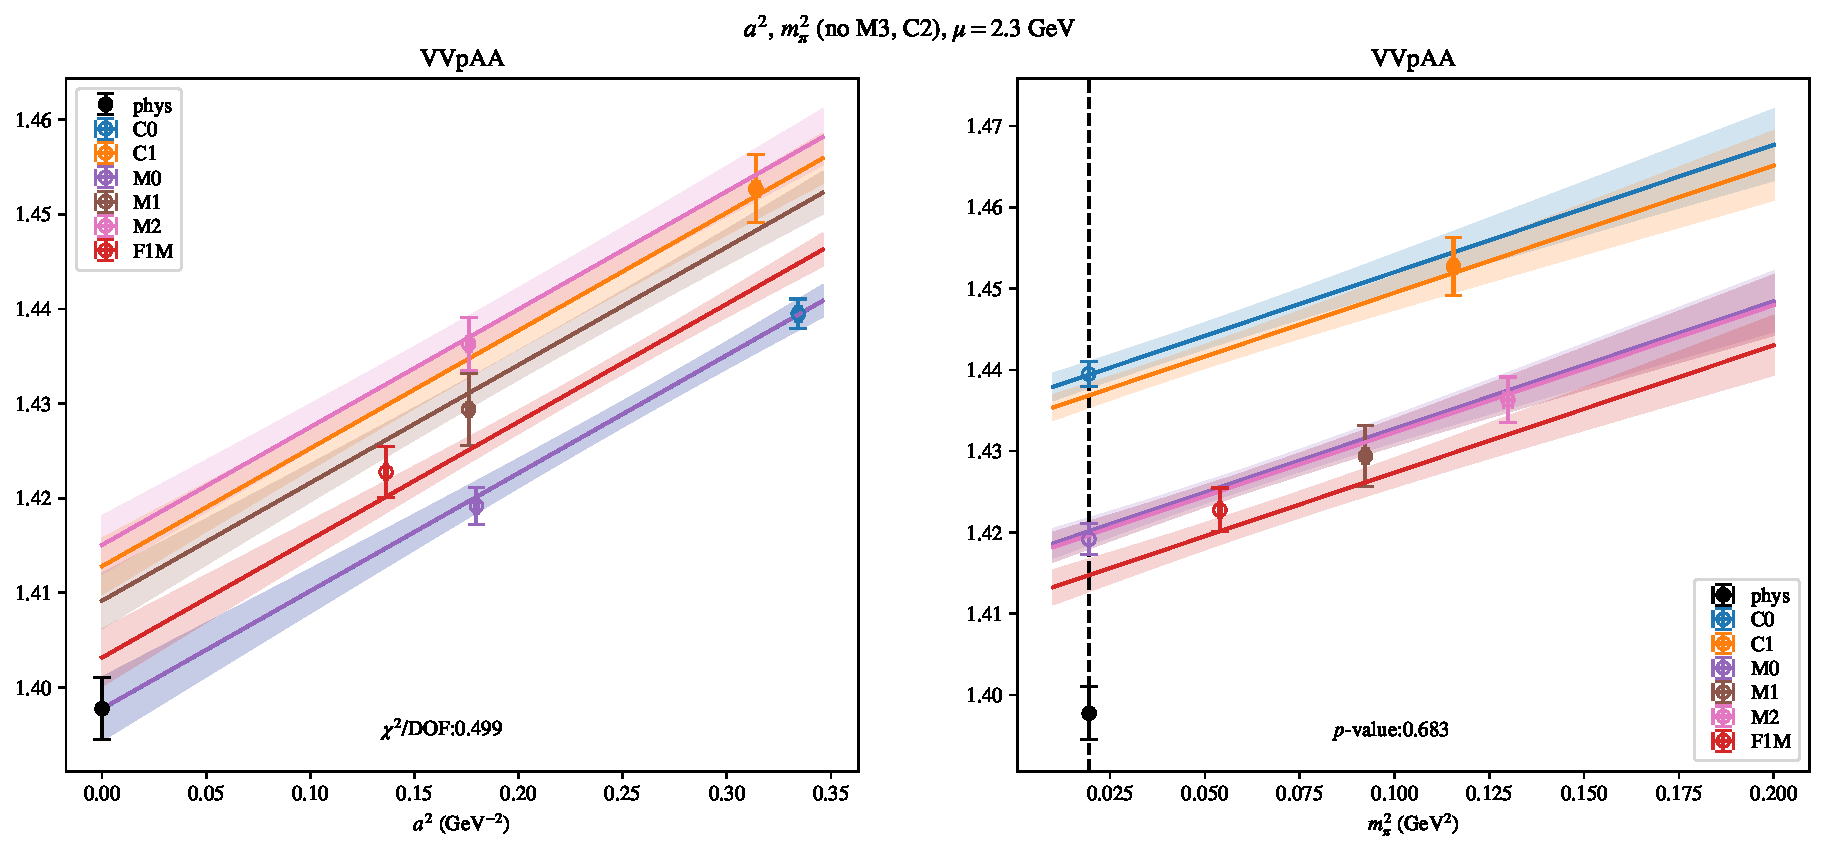
\includepdf[link, pages=-]{VVpAA/NPR/bag_a2m2mcut_23.pdf}
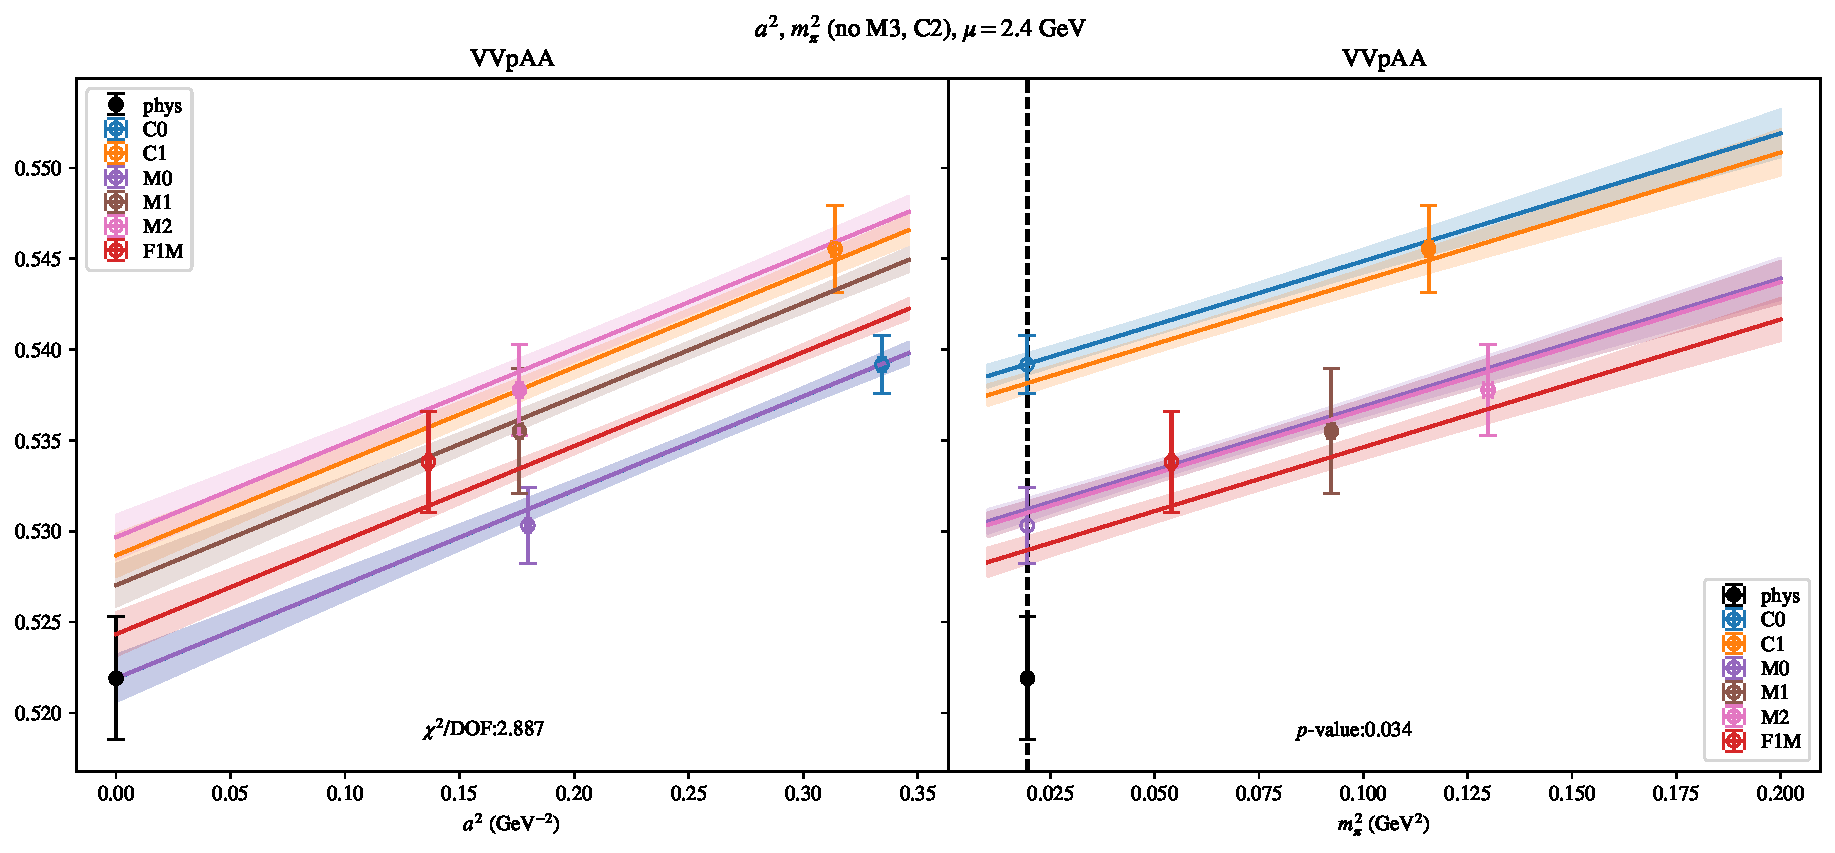
\includepdf[link, pages=-]{VVpAA/NPR/bag_a2m2mcut_24.pdf}
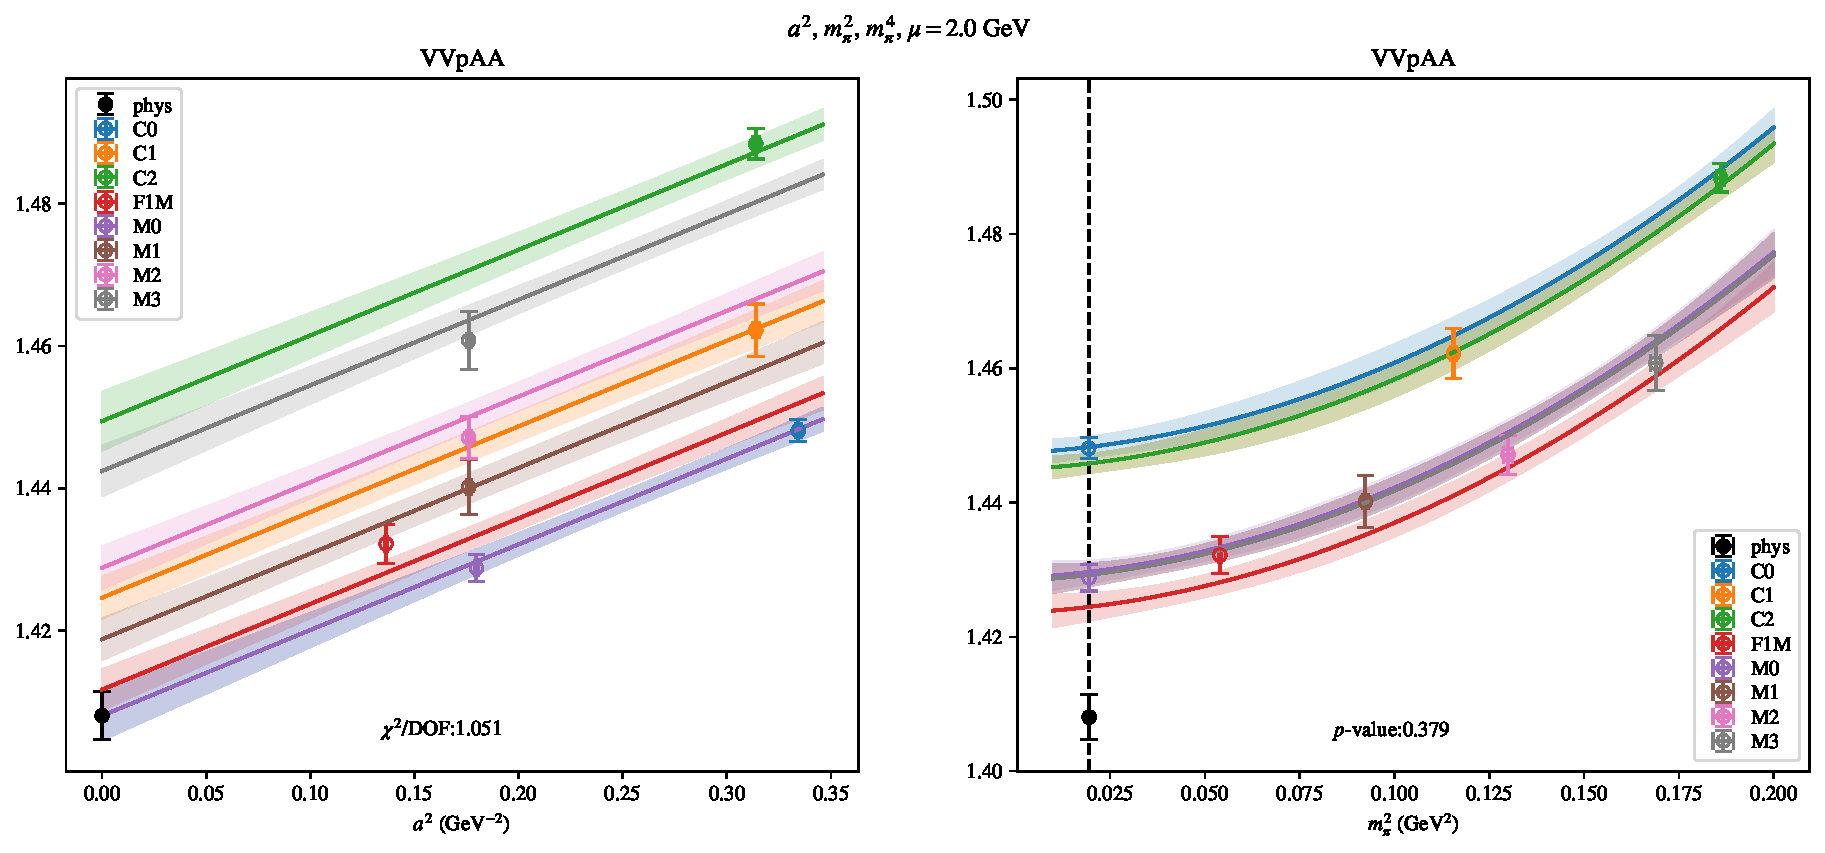
\includepdf[link, pages=-]{VVpAA/NPR/bag_a2m2m4_20.pdf}
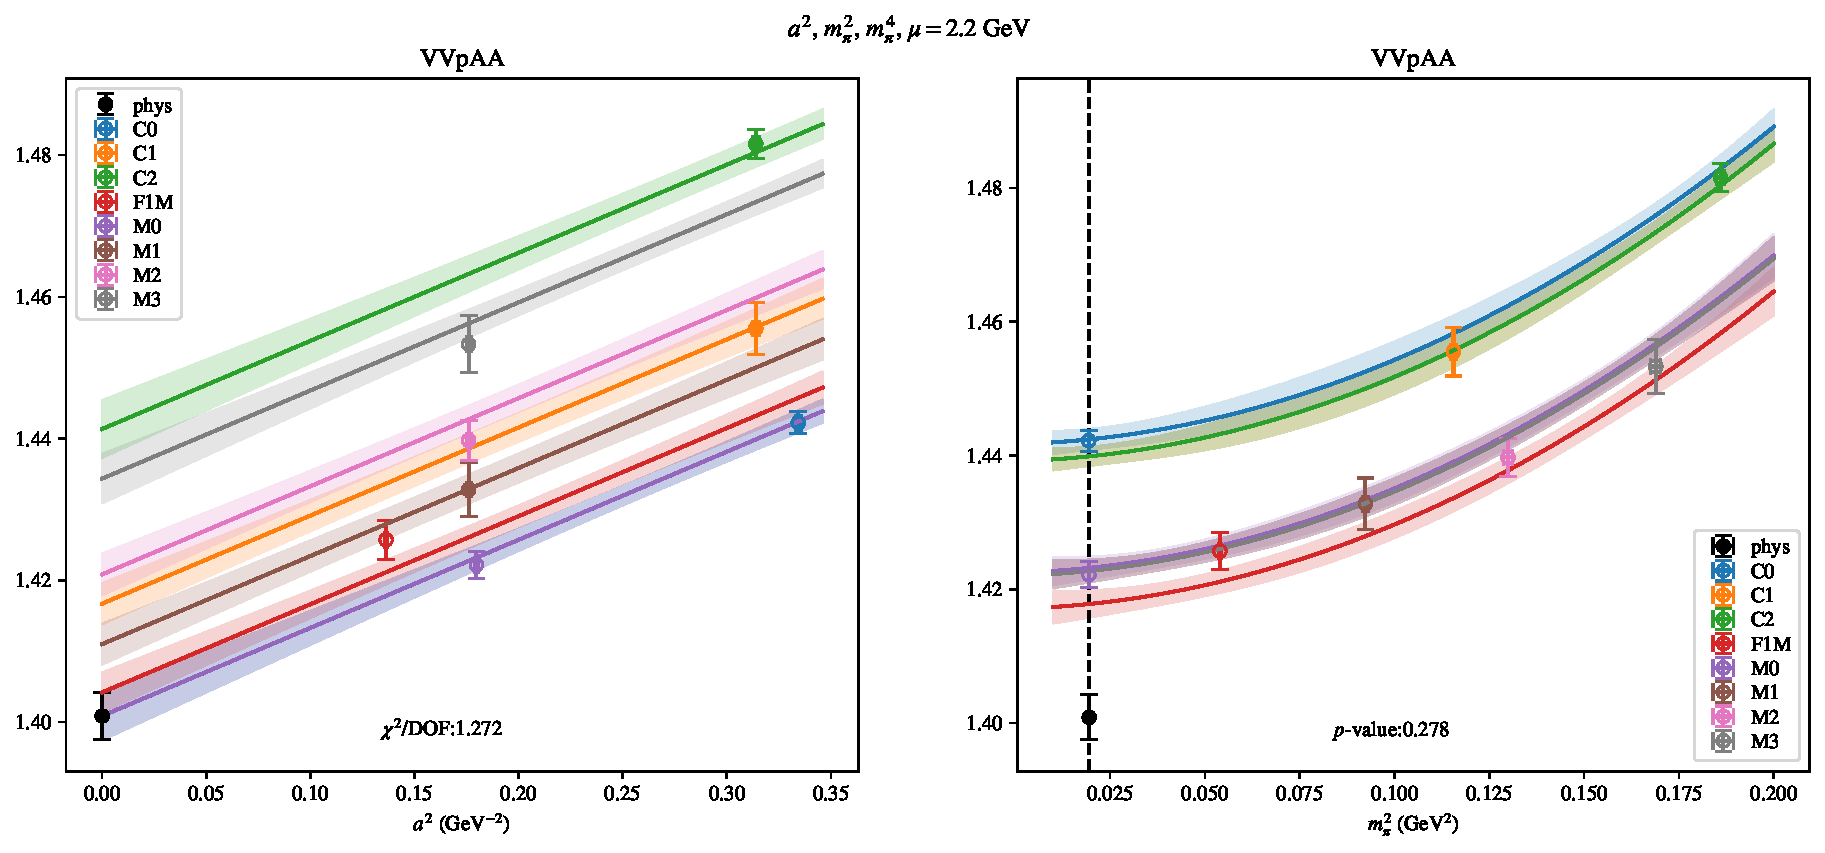
\includepdf[link, pages=-]{VVpAA/NPR/bag_a2m2m4_22.pdf}
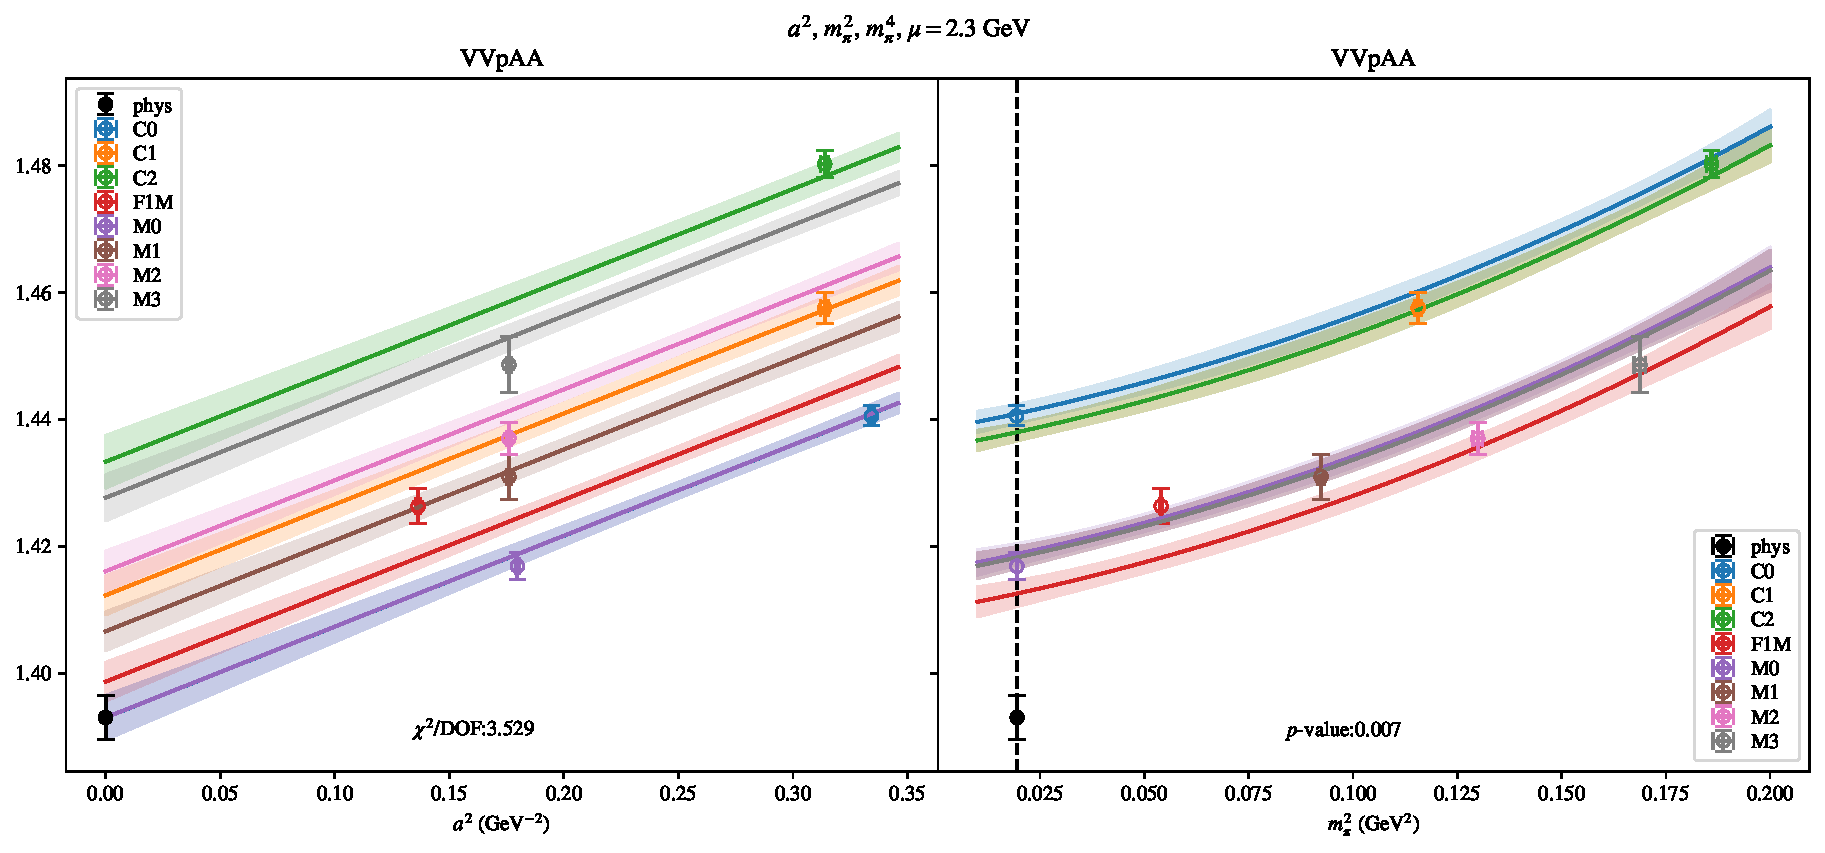
\includepdf[link, pages=-]{VVpAA/NPR/bag_a2m2m4_23.pdf}
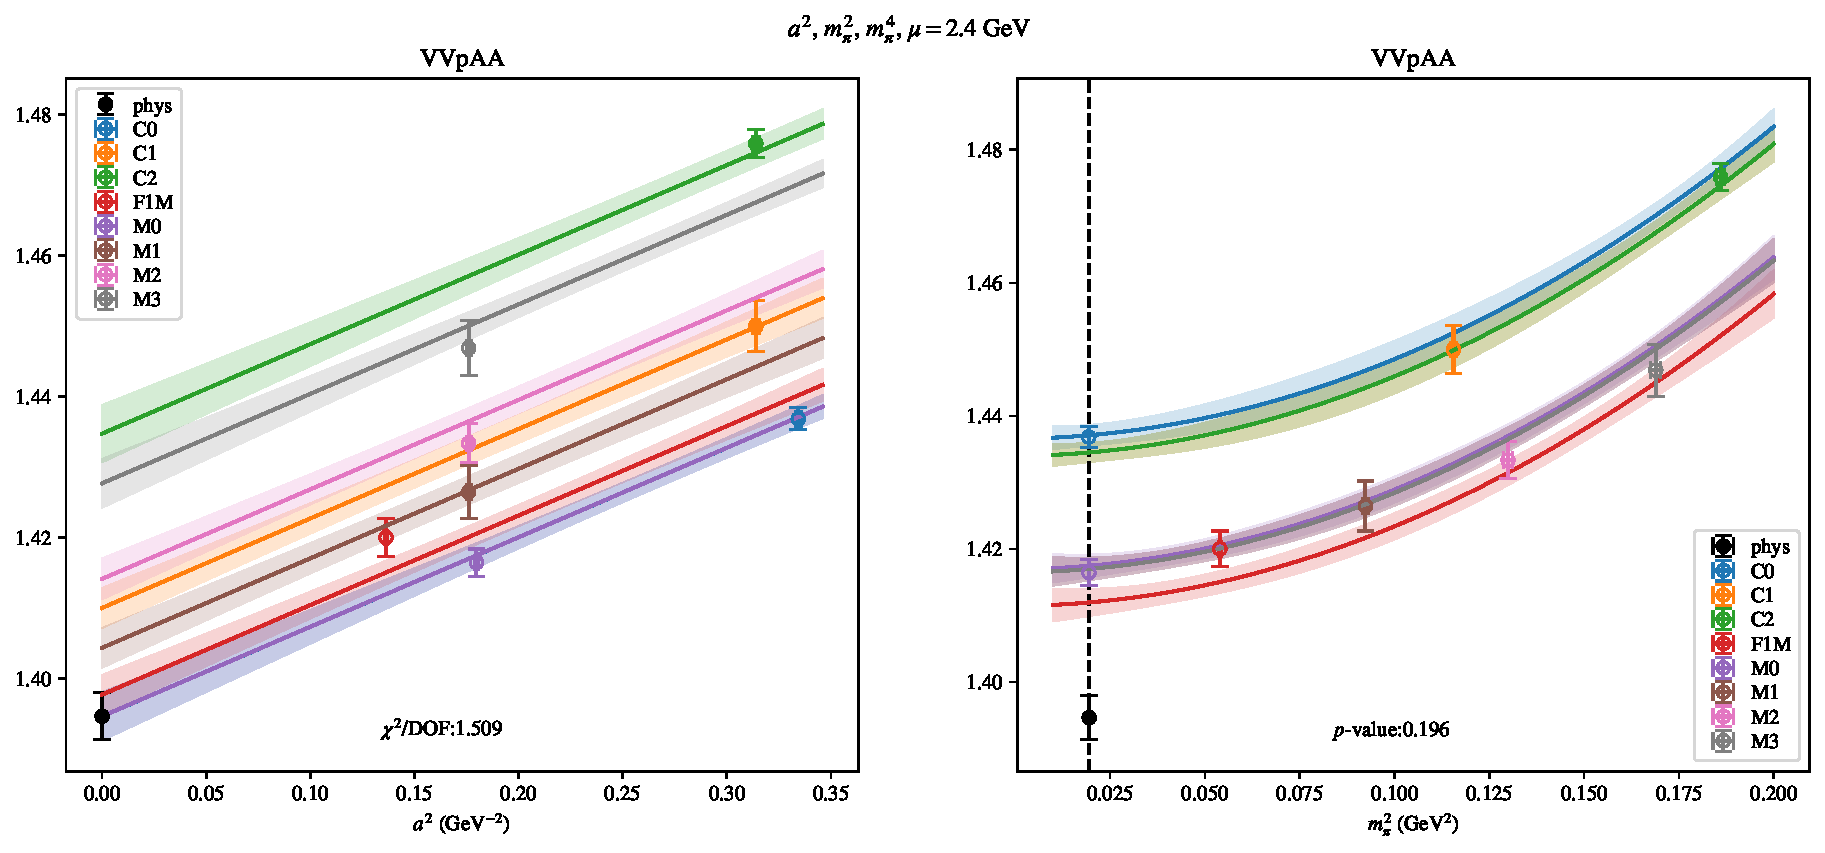
\includepdf[link, pages=-]{VVpAA/NPR/bag_a2m2m4_24.pdf}
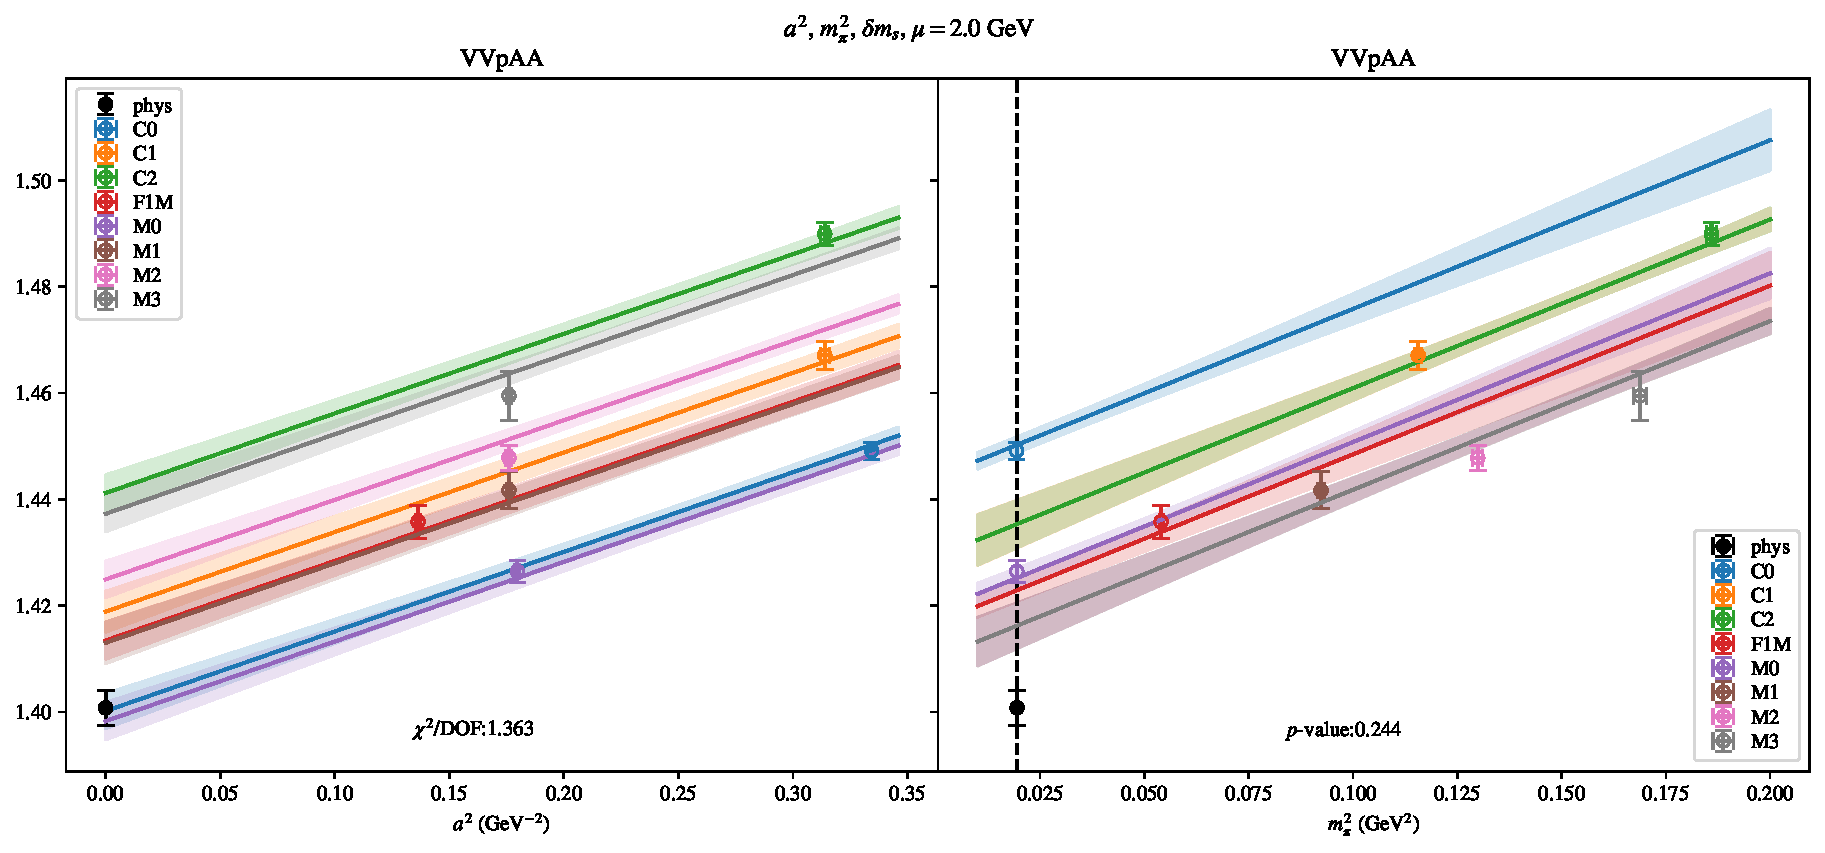
\includepdf[link, pages=-]{VVpAA/NPR/bag_a2m2delm_20.pdf}
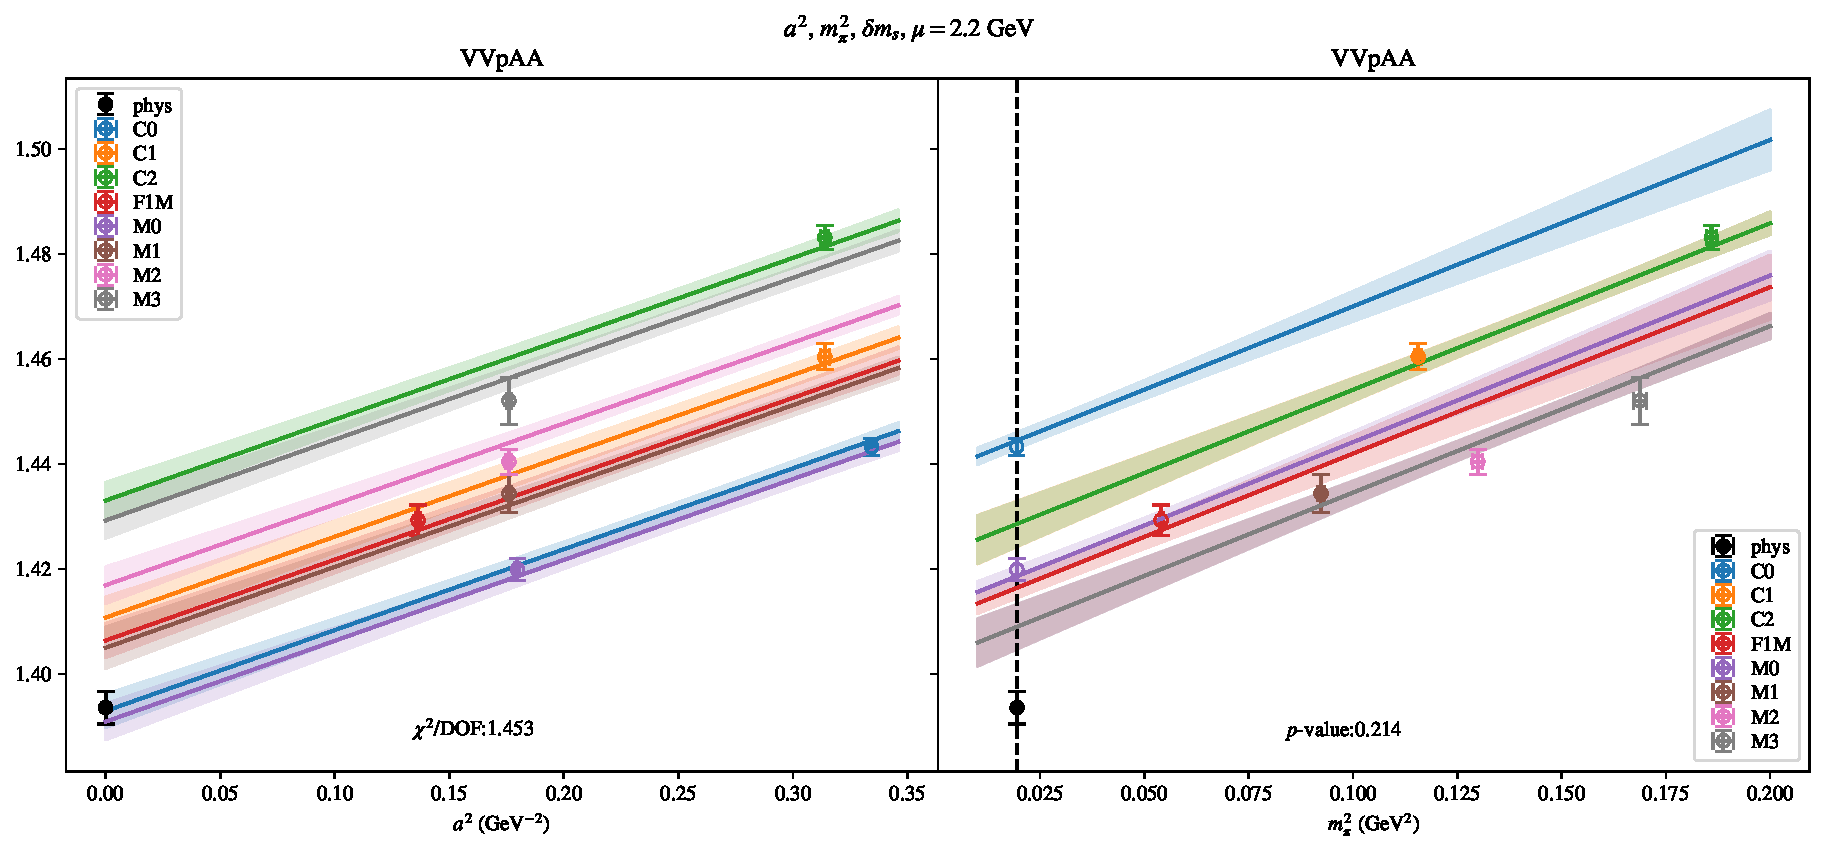
\includepdf[link, pages=-]{VVpAA/NPR/bag_a2m2delm_22.pdf}
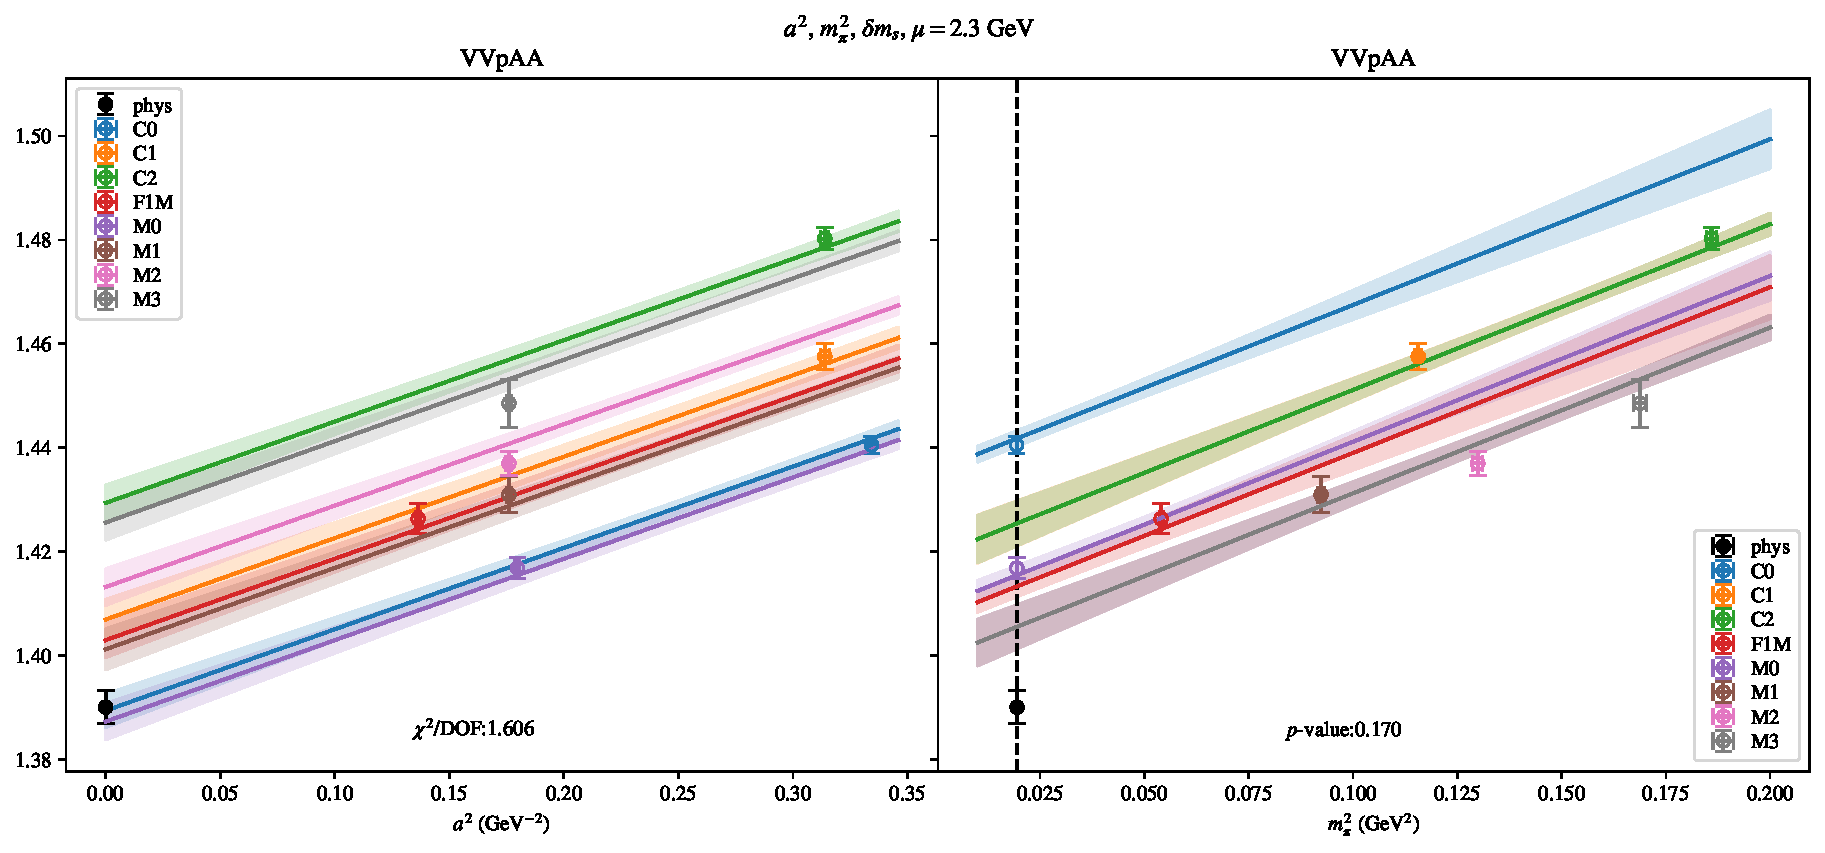
\includepdf[link, pages=-]{VVpAA/NPR/bag_a2m2delm_23.pdf}
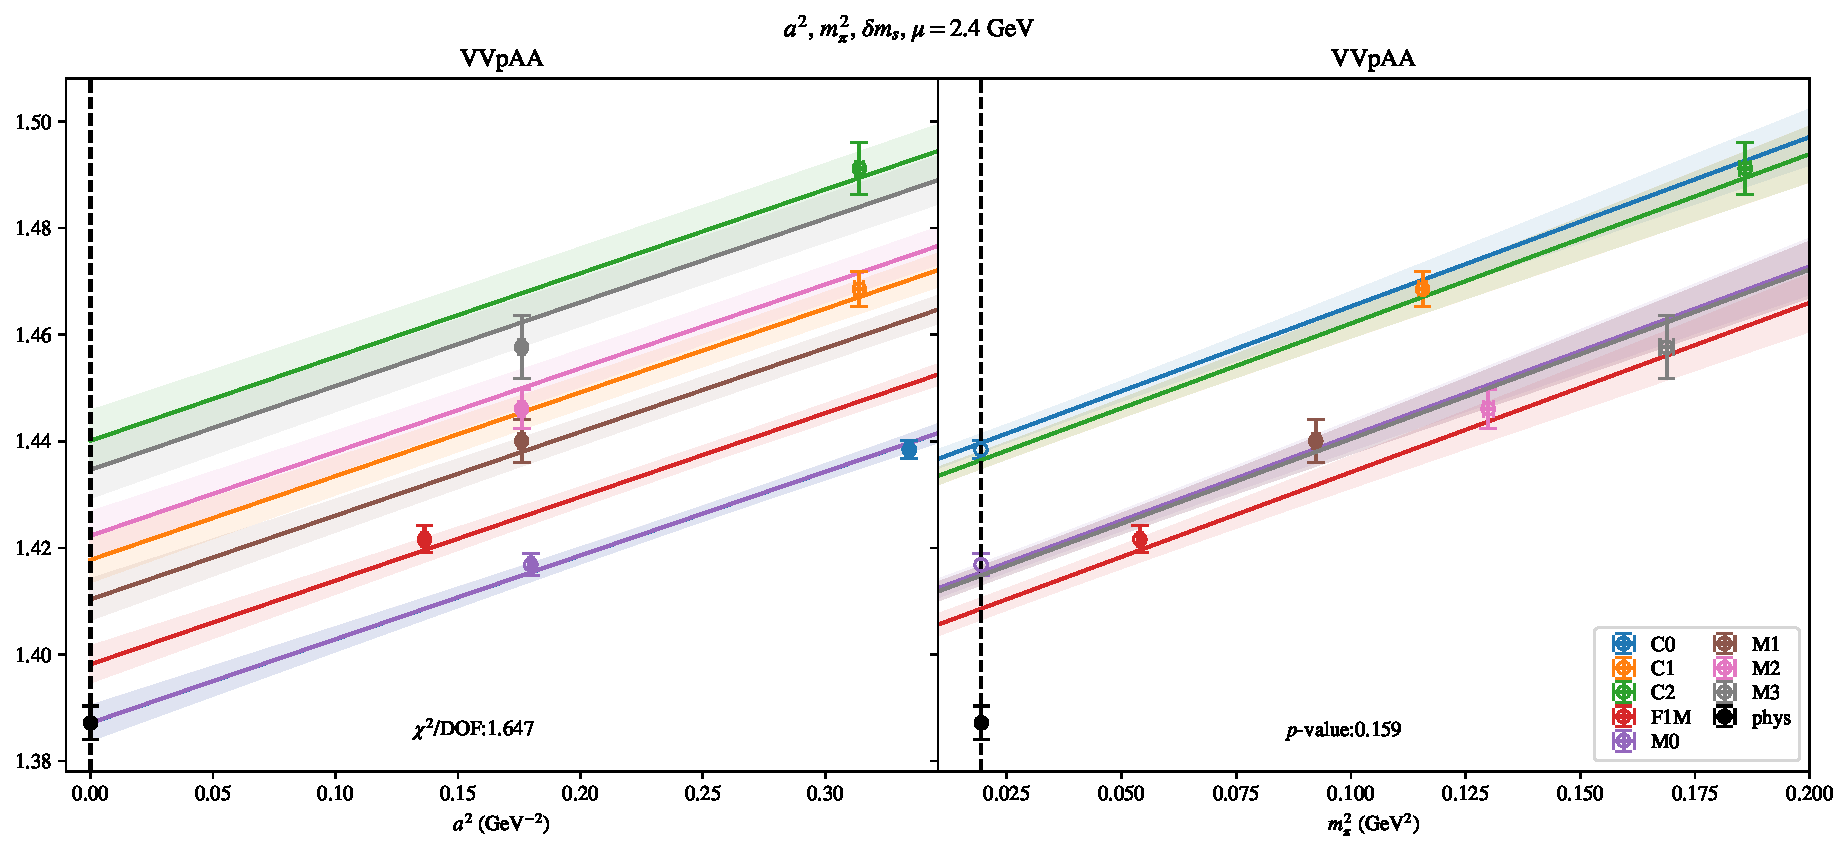
\includepdf[link, pages=-]{VVpAA/NPR/bag_a2m2delm_24.pdf}
\clearpage
\section{$\mathcal{B}_2$}
\begin{table}[h!]
\begin{center}
\begin{tabular}{|c|c|c|c|c|c|c|}
\hline
$\mu$ (GeV) & $a^2$, $m_\pi^2$& $a^2$, $m_\pi^2$ (no C)& $a^2$, $m_\pi^2$, $a^4$& $a^2$, $m_\pi^2$ (no M3, C2)& $a^2$, $m_\pi^2$, $m_\pi^4$& $a^2$, $m_\pi^2$, $\delta m_s$\\
\hline
2.0& \hyperlink{VVmAA/NPR/bag_a2m2_20.pdf.1}{\textbf{-0.9859(80)}: 0.381 (0.862)} & \hyperlink{VVmAA/NPR/bag_a2m2noC_20.pdf.1}{\textbf{-0.941(37)}: 0.091 (0.913)} & \hyperlink{VVmAA/NPR/bag_a2a4m2_20.pdf.1}{\textbf{-0.916(57)}: 0.129 (0.972)} & \hyperlink{VVmAA/NPR/bag_a2m2mcut_20.pdf.1}{\textbf{-0.9867(91)}: 0.607 (0.61)} & \hyperlink{VVmAA/NPR/bag_a2m2m4_20.pdf.1}{\textbf{-0.9877(86)}: 0.427 (0.789)} & \hyperlink{VVmAA/NPR/bag_a2m2delm_20.pdf.1}{\textbf{-0.9861(79)}: 0.346 (0.847)}\\
2.2& \hyperlink{VVmAA/NPR/bag_a2m2_22.pdf.1}{\textbf{-1.0005(70)}: 0.396 (0.852)} & \hyperlink{VVmAA/NPR/bag_a2m2noC_22.pdf.1}{\textbf{-0.961(31)}: 0.045 (0.956)} & \hyperlink{VVmAA/NPR/bag_a2a4m2_22.pdf.1}{\textbf{-0.940(51)}: 0.157 (0.96)} & \hyperlink{VVmAA/NPR/bag_a2m2mcut_22.pdf.1}{\textbf{-1.0008(78)}: 0.624 (0.6)} & \hyperlink{VVmAA/NPR/bag_a2m2m4_22.pdf.1}{\textbf{-1.0025(74)}: 0.369 (0.831)} & \hyperlink{VVmAA/NPR/bag_a2m2delm_22.pdf.1}{\textbf{-1.0002(72)}: 0.418 (0.796)}\\
2.3& \hyperlink{VVmAA/NPR/bag_a2m2_23.pdf.1}{\textbf{-1.0069(63)}: 0.423 (0.833)} & \hyperlink{VVmAA/NPR/bag_a2m2noC_23.pdf.1}{\textbf{-0.968(29)}: 0.05 (0.951)} & \hyperlink{VVmAA/NPR/bag_a2a4m2_23.pdf.1}{\textbf{-0.947(48)}: 0.13 (0.972)} & \hyperlink{VVmAA/NPR/bag_a2m2mcut_23.pdf.1}{\textbf{-1.0076(70)}: 0.65 (0.583)} & \hyperlink{VVmAA/NPR/bag_a2m2m4_23.pdf.1}{\textbf{-1.0088(72)}: 0.409 (0.802)} & \hyperlink{VVmAA/NPR/bag_a2m2delm_23.pdf.1}{\textbf{-1.0065(64)}: 0.419 (0.795)}\\
2.4& \hyperlink{VVmAA/NPR/bag_a2m2_24.pdf.1}{\textbf{-1.0117(60)}: 0.444 (0.818)} & \hyperlink{VVmAA/NPR/bag_a2m2noC_24.pdf.1}{\textbf{-0.975(26)}: 0.05 (0.951)} & \hyperlink{VVmAA/NPR/bag_a2a4m2_24.pdf.1}{\textbf{-0.957(45)}: 0.164 (0.956)} & \hyperlink{VVmAA/NPR/bag_a2m2mcut_24.pdf.1}{\textbf{-1.0123(67)}: 0.676 (0.567)} & \hyperlink{VVmAA/NPR/bag_a2m2m4_24.pdf.1}{\textbf{-1.0139(66)}: 0.433 (0.785)} & \hyperlink{VVmAA/NPR/bag_a2m2delm_24.pdf.1}{\textbf{-1.0121(58)}: 0.445 (0.776)}\\
\hline
\end{tabular}
\caption{Physical point value from chiral and continuum extrapolation at renormalisation scale $\mu$. Entries are \textbf{value(error)}: $\chi^2/\text{DOF}$ ($p$-value).}
\end{center}
\end{table}
\begin{table}[h!]
\begin{center}
\begin{tabular}{|c c|c|c|c|c|c|c|}
\hline
$\mu$ (GeV) &  & $a^2$, $m_\pi^2$& $a^2$, $m_\pi^2$ (no C)& $a^2$, $m_\pi^2$, $a^4$& $a^2$, $m_\pi^2$ (no M3, C2)& $a^2$, $m_\pi^2$, $m_\pi^4$& $a^2$, $m_\pi^2$, $\delta m_s$\\
\hline
\multirow{3}{0.5in}{2.0} & $\alpha$ & 0.167(28)& -0.10(21)& -0.48(53)& 0.169(31)& 0.172(28)& 0.170(27)\\
 & $\beta$ & -0.00148(53)& -0.0013(11)& -0.00108(59)& -0.00144(89)& -0.0005(26)& -0.0007(11)\\
 & $\gamma$ &  &  & 1.3(10)&  & -0.00008(22)& -0.029(41)\\
\hline
\multirow{3}{0.5in}{2.2} & $\alpha$ & 0.212(24)& -0.03(18)& -0.34(47)& 0.212(26)& 0.217(24)& 0.213(24)\\
 & $\beta$ & -0.00158(46)& -0.00138(90)& -0.00124(55)& -0.00137(74)& -0.0002(22)& -0.0012(10)\\
 & $\gamma$ &  &  & 1.13(96)&  & -0.00012(19)& -0.017(35)\\
\hline
\multirow{3}{0.5in}{2.3} & $\alpha$ & 0.236(21)& -0.00005(17357)& -0.32(44)& 0.238(24)& 0.241(23)& 0.237(22)\\
 & $\beta$ & -0.00156(42)& -0.00138(80)& -0.00122(49)& -0.00139(70)& -0.0005(20)& -0.00107(92)\\
 & $\gamma$ &  &  & 1.13(89)&  & -0.00010(17)& -0.020(32)\\
\hline
\multirow{3}{0.5in}{2.4} & $\alpha$ & 0.258(20)& 0.03(15)& -0.25(41)& 0.259(22)& 0.264(21)& 0.261(20)\\
 & $\beta$ & -0.00154(38)& -0.00140(77)& -0.00121(45)& -0.00139(64)& -0.0006(18)& -0.00110(81)\\
 & $\gamma$ &  &  & 1.03(85)&  & -0.00009(16)& -0.017(29)\\
\hline
\end{tabular}
\caption{Fit values of coefficients in $Q = Q_{phys} + \mathbf{\alpha} a^2 + \mathbf{\beta}\left(\frac{m_\pi^2}{f_\pi^2}-\frac{m_{\pi,PDG}^2}{f_\pi^2}\right) + \gamma(\ldots)$}
\end{center}
\end{table}
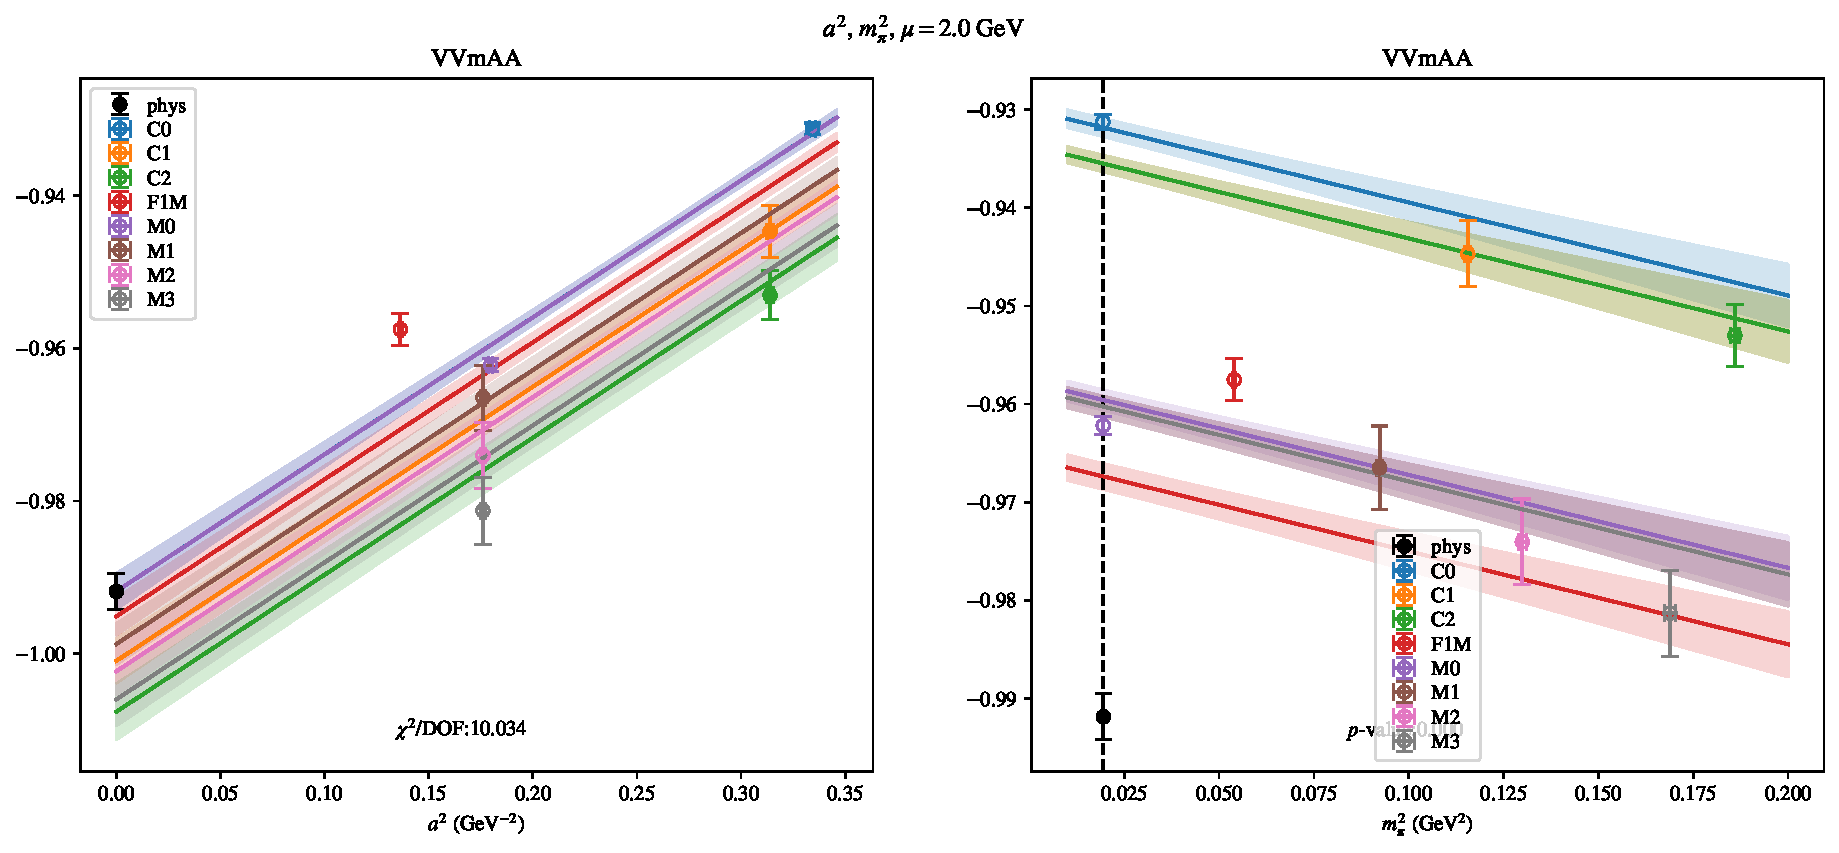
\includepdf[link, pages=-]{VVmAA/NPR/bag_a2m2_20.pdf}
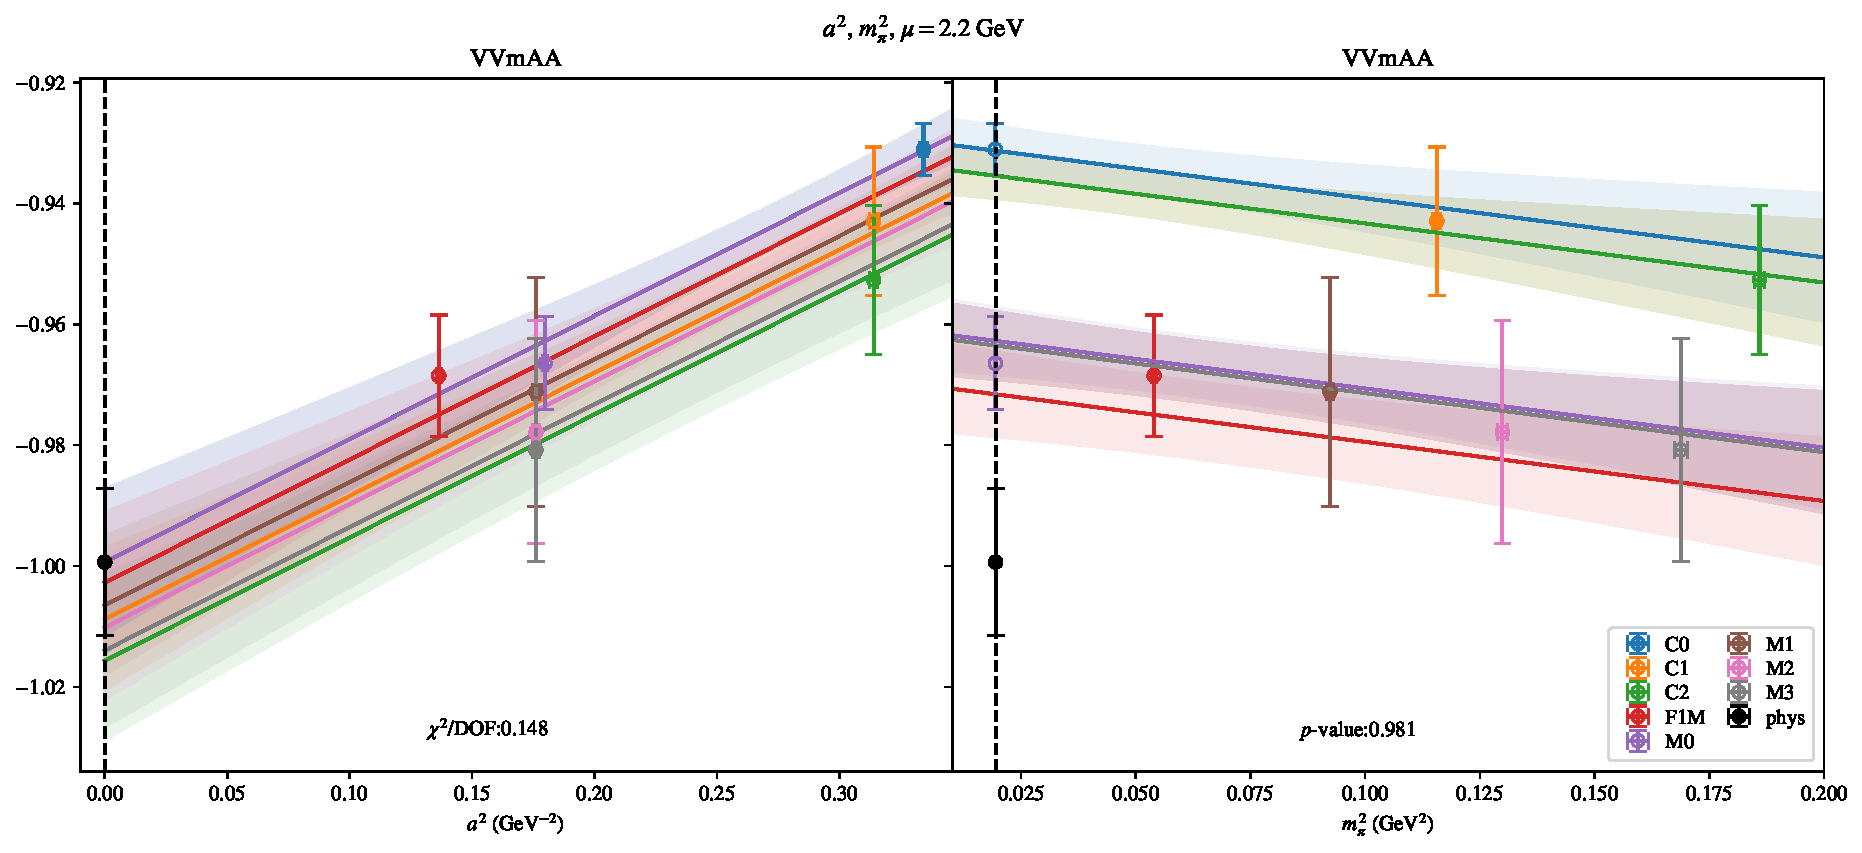
\includepdf[link, pages=-]{VVmAA/NPR/bag_a2m2_22.pdf}
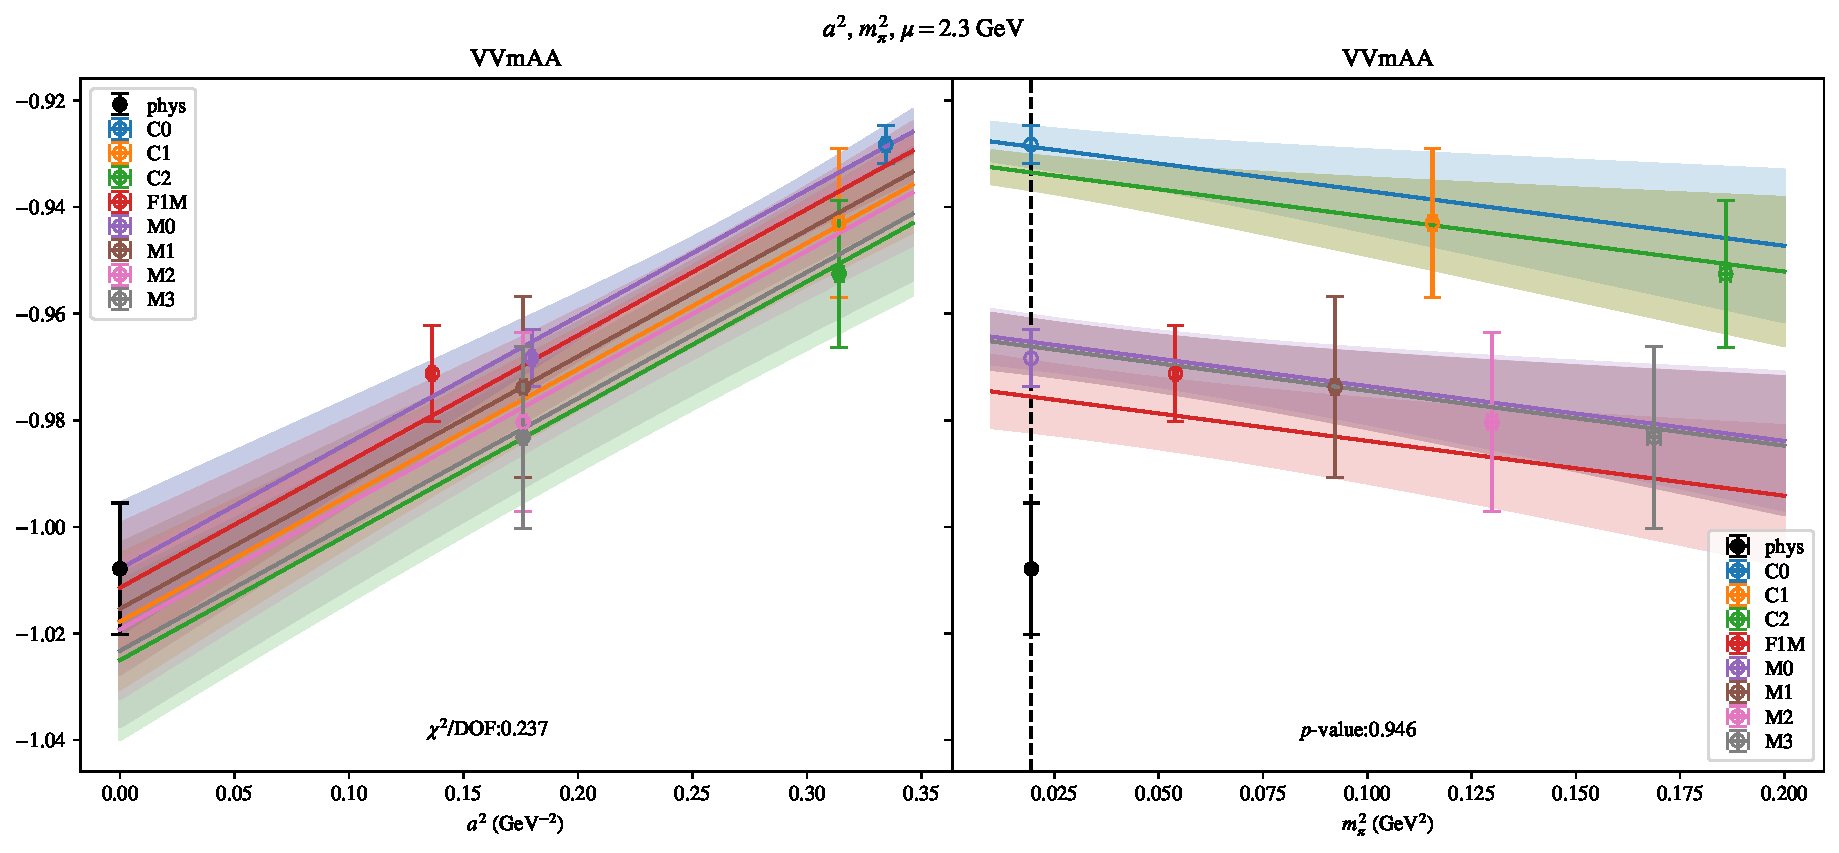
\includepdf[link, pages=-]{VVmAA/NPR/bag_a2m2_23.pdf}
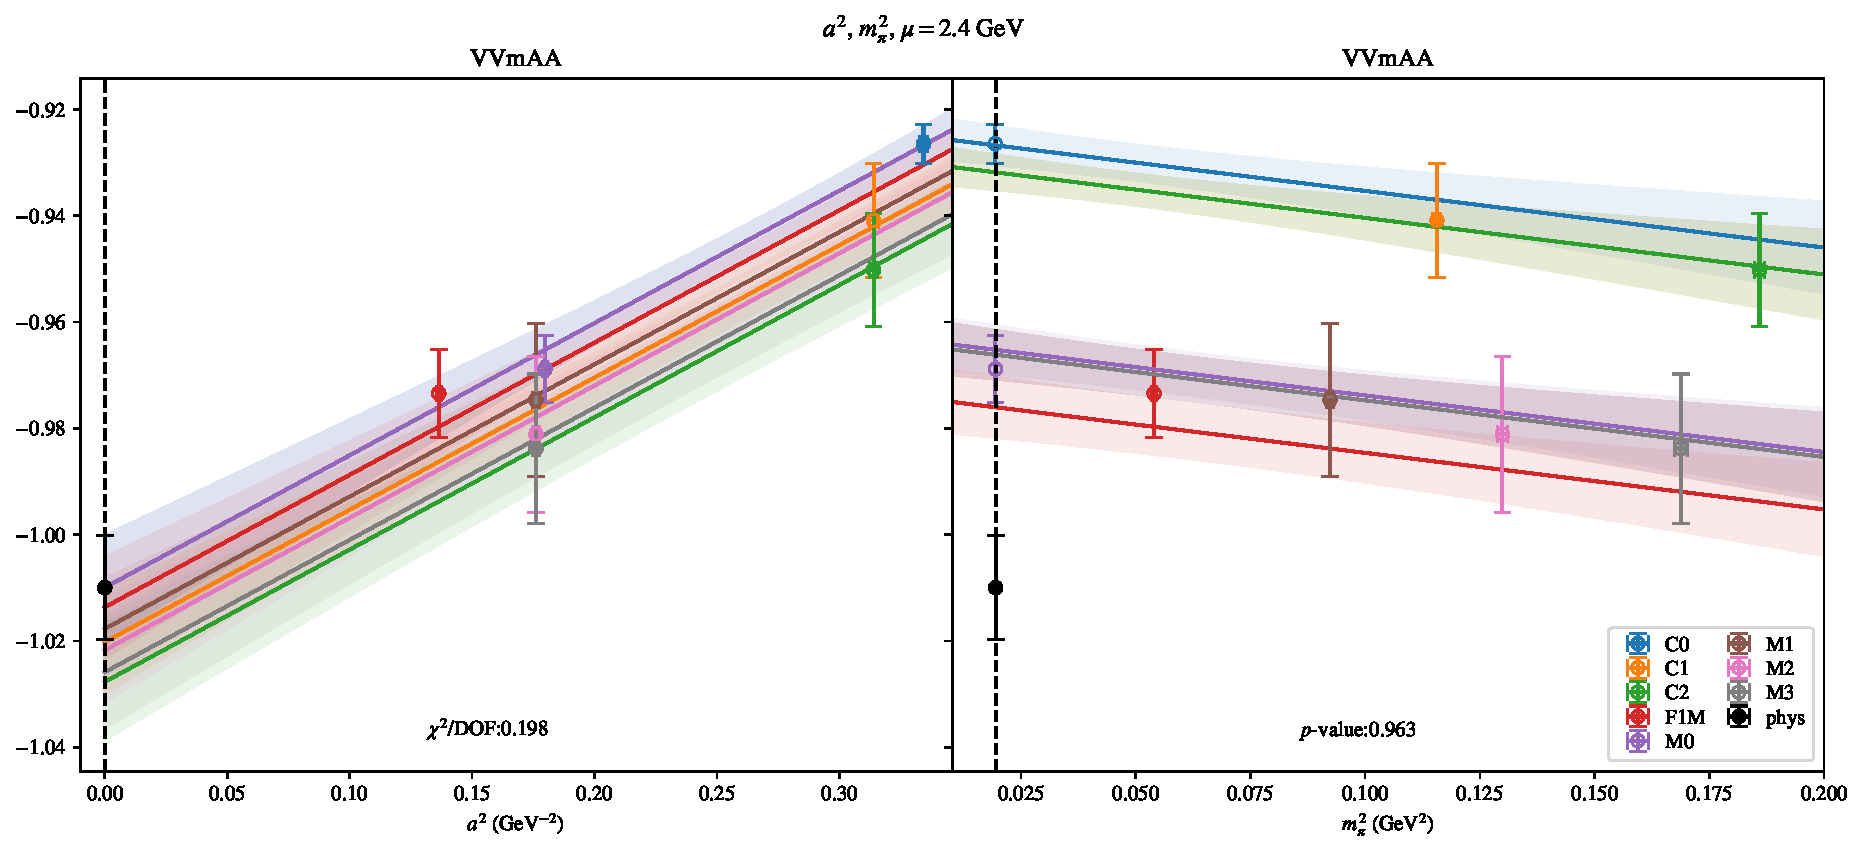
\includepdf[link, pages=-]{VVmAA/NPR/bag_a2m2_24.pdf}
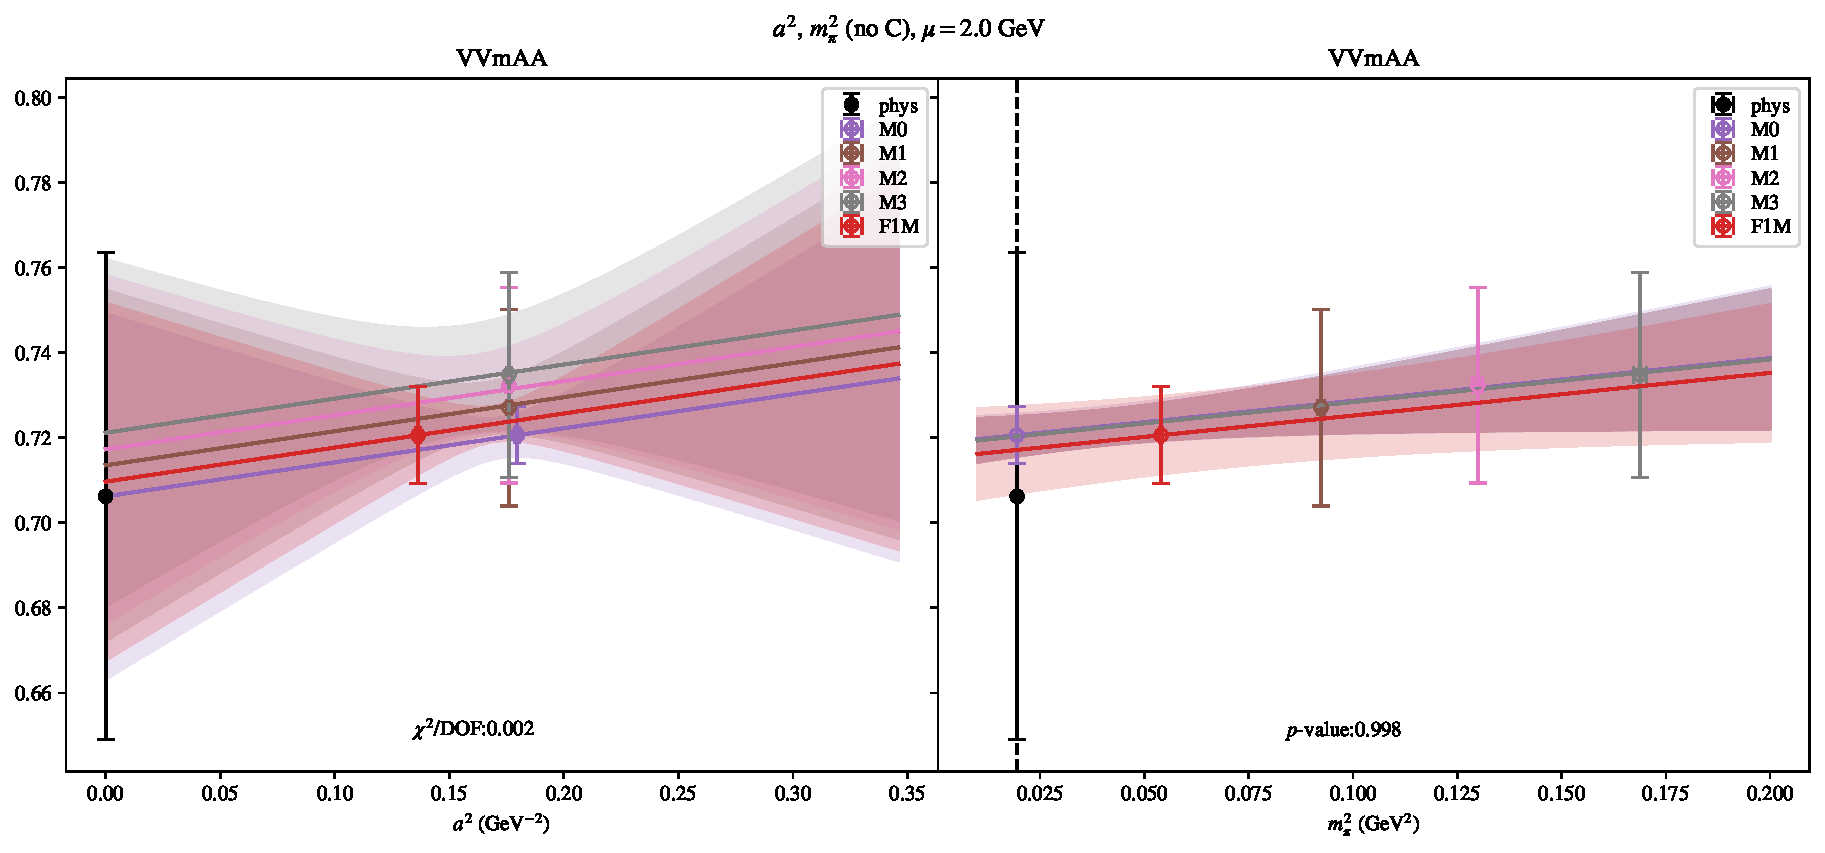
\includepdf[link, pages=-]{VVmAA/NPR/bag_a2m2noC_20.pdf}
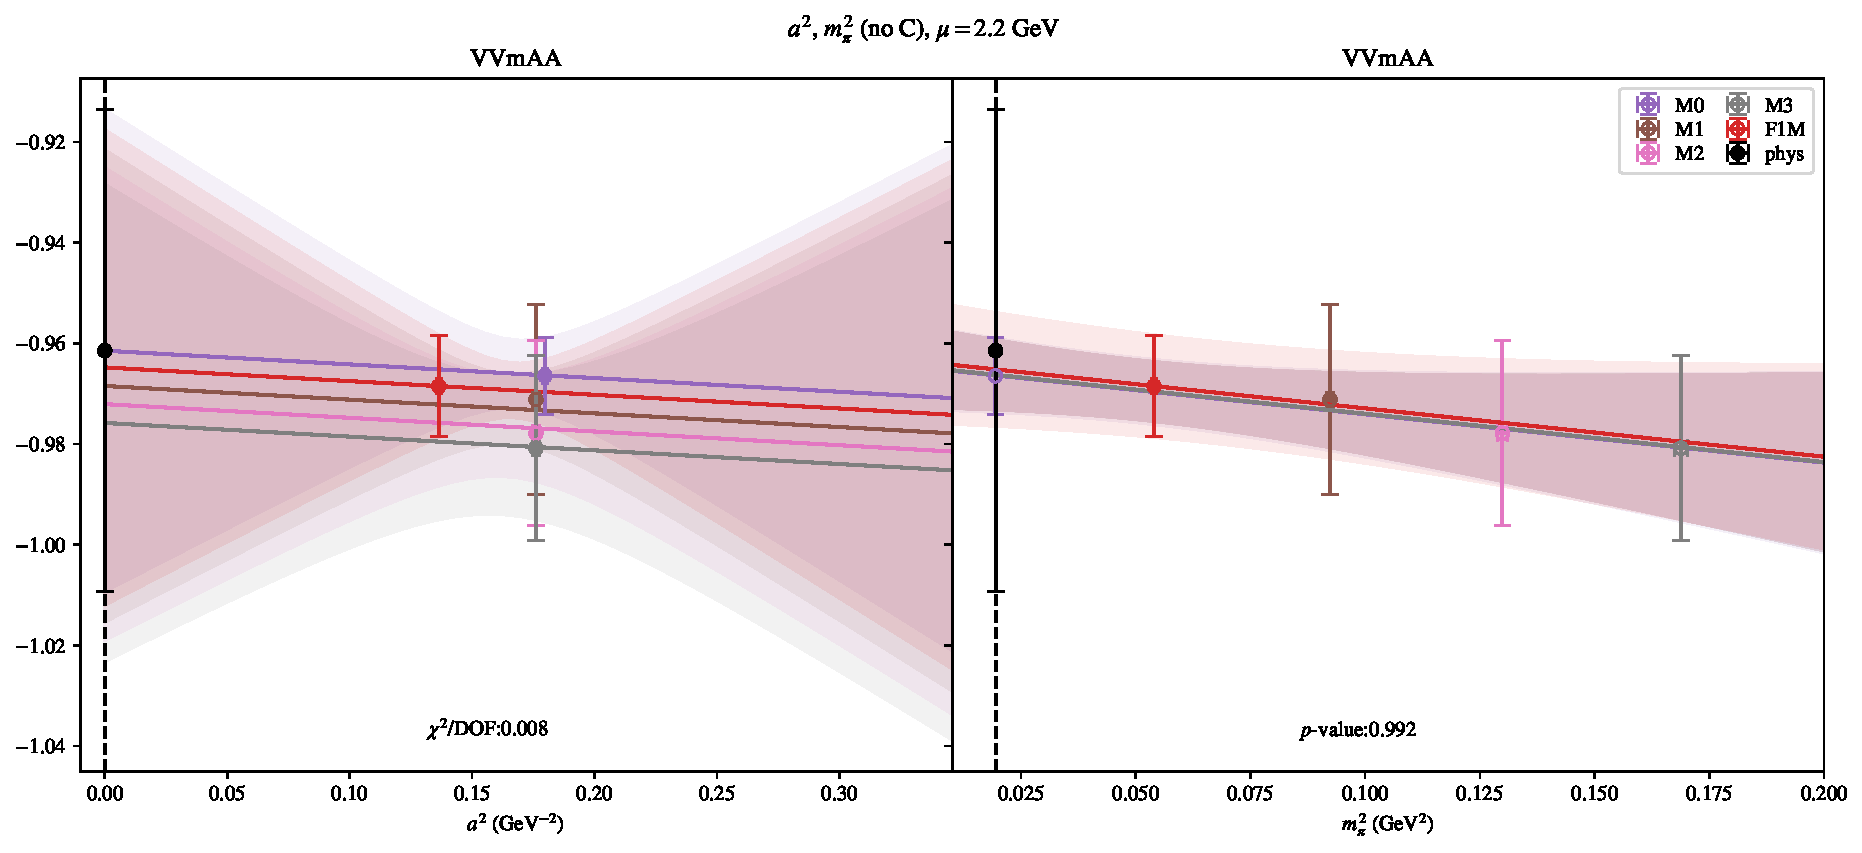
\includepdf[link, pages=-]{VVmAA/NPR/bag_a2m2noC_22.pdf}
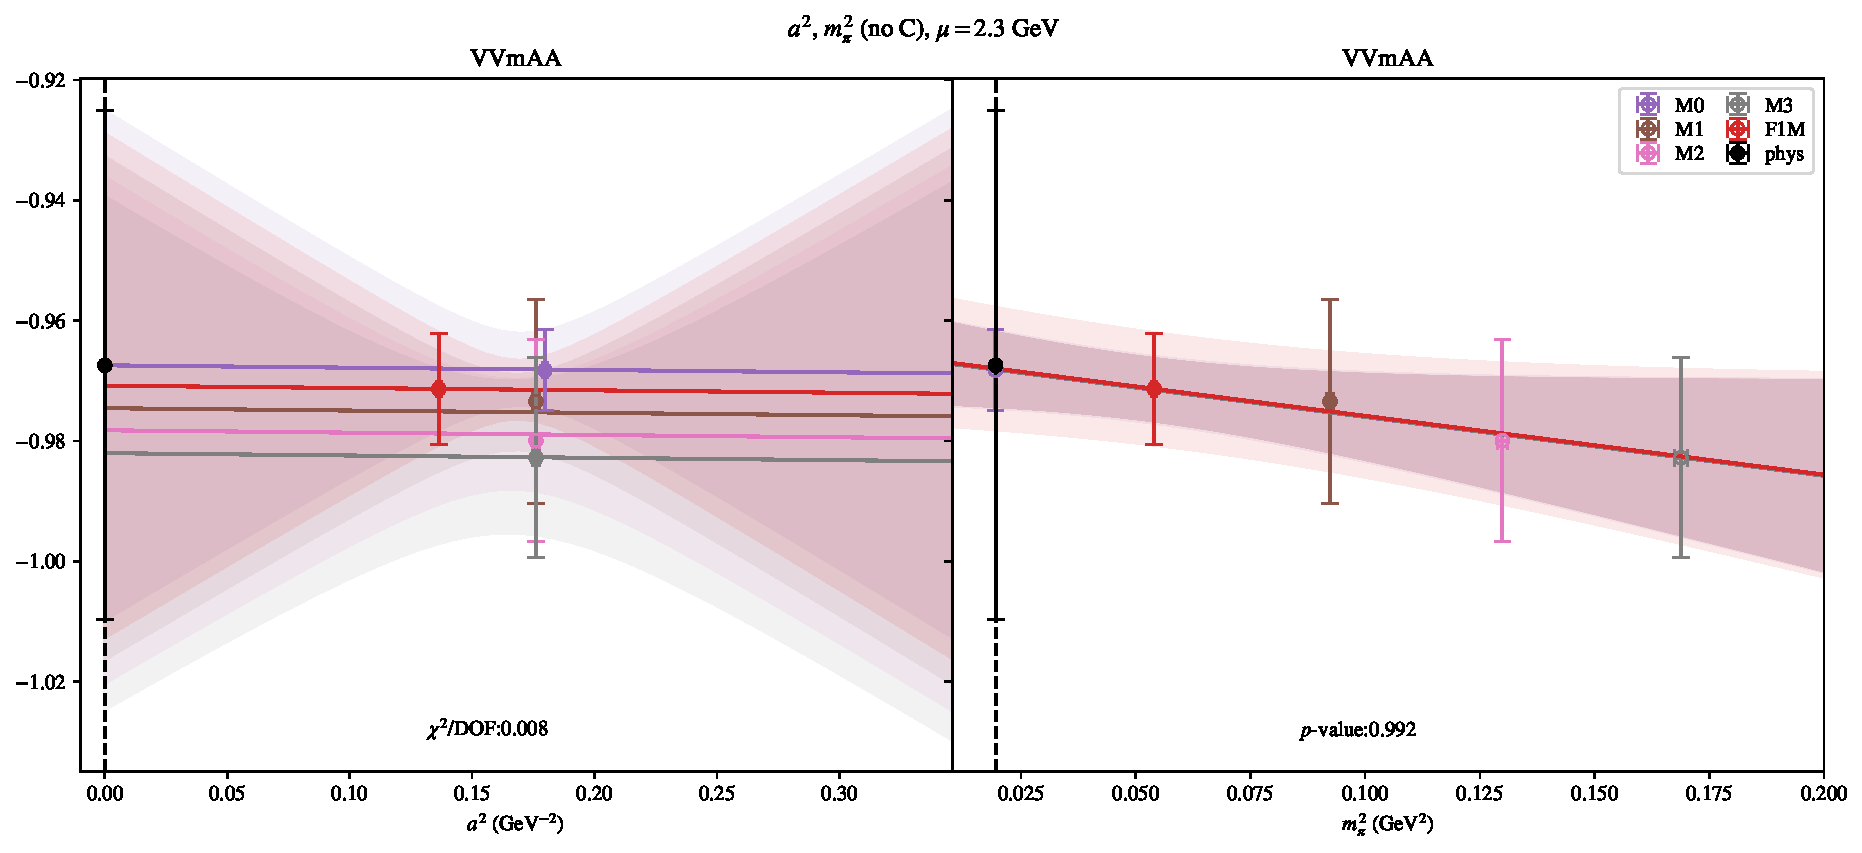
\includepdf[link, pages=-]{VVmAA/NPR/bag_a2m2noC_23.pdf}
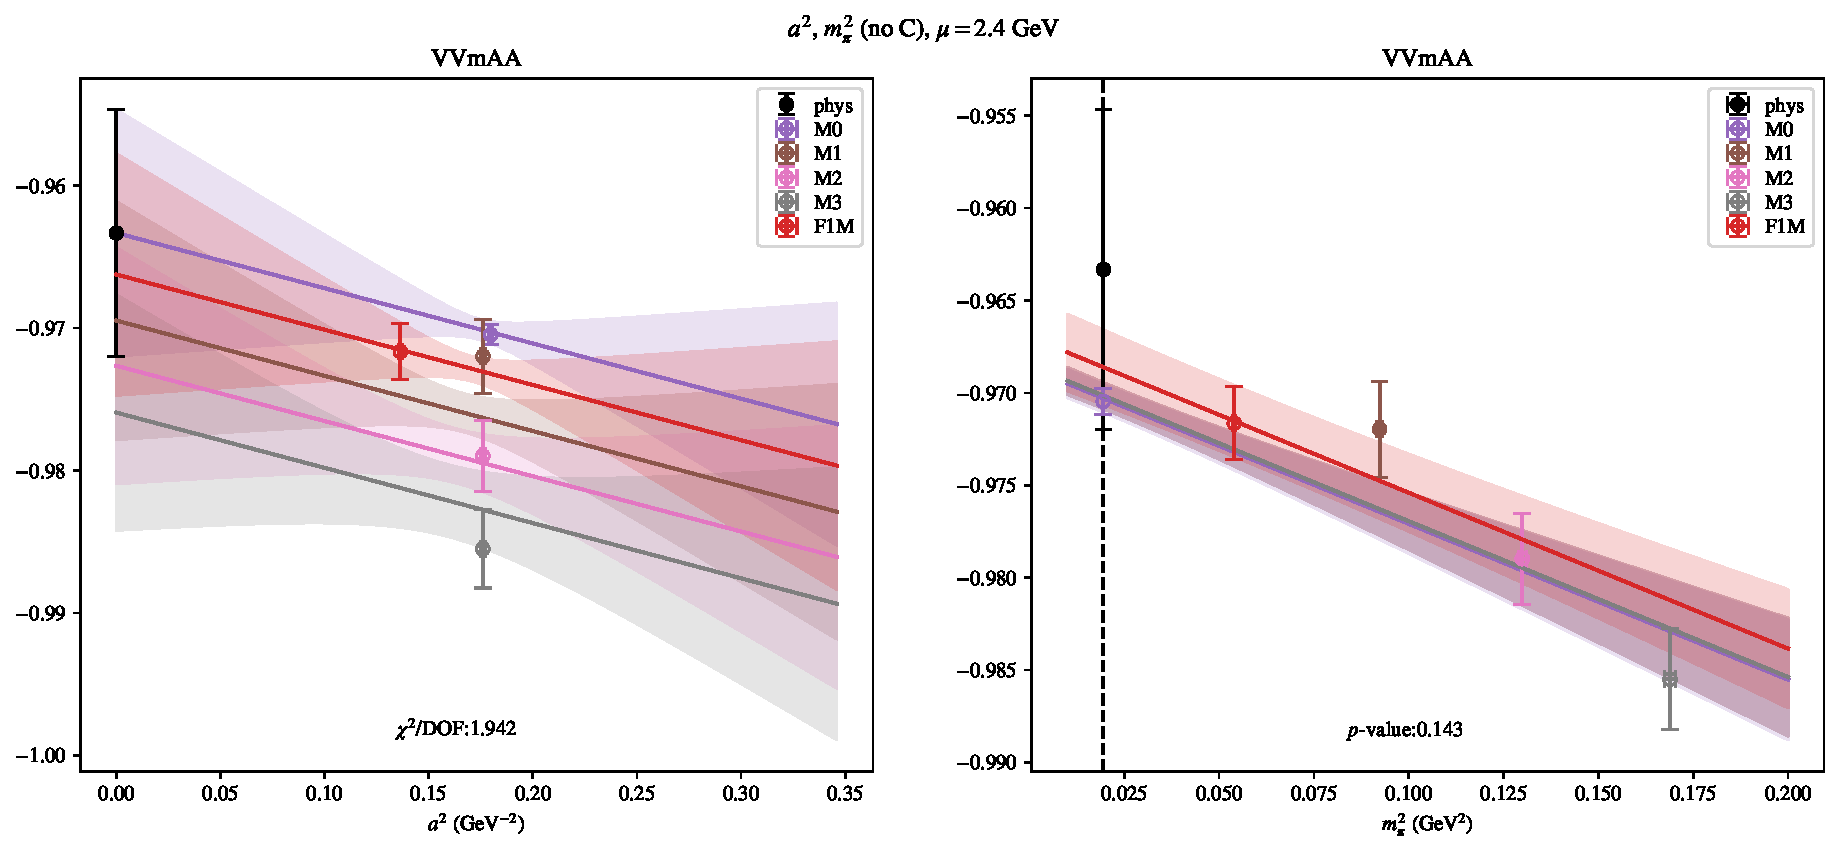
\includepdf[link, pages=-]{VVmAA/NPR/bag_a2m2noC_24.pdf}
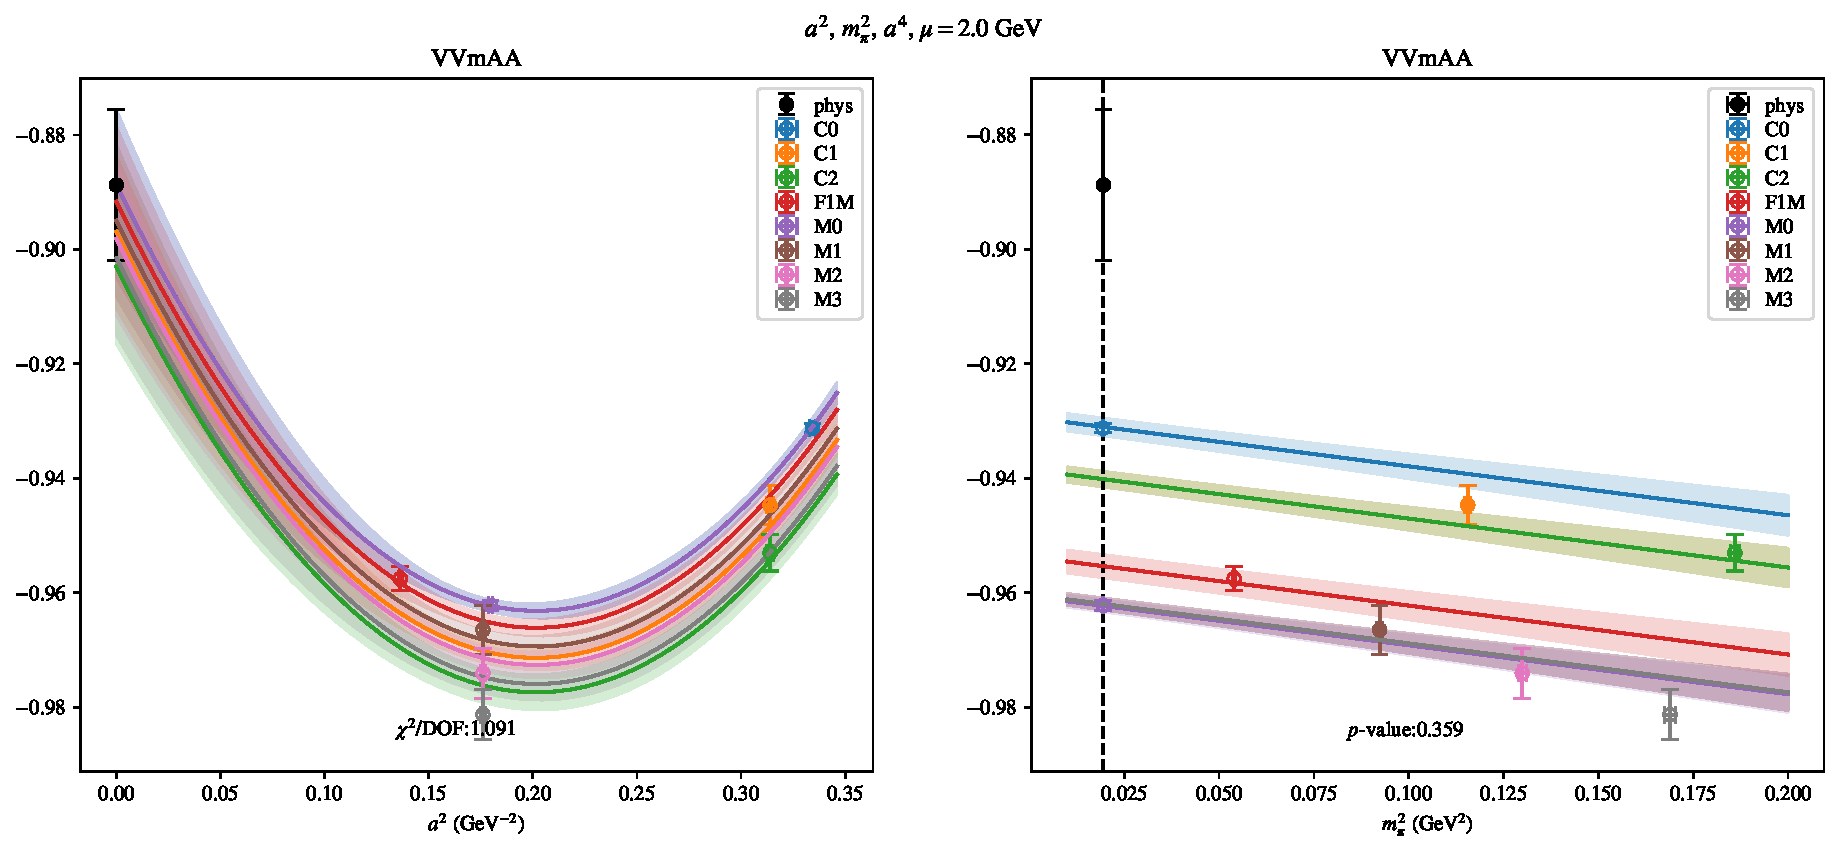
\includepdf[link, pages=-]{VVmAA/NPR/bag_a2a4m2_20.pdf}
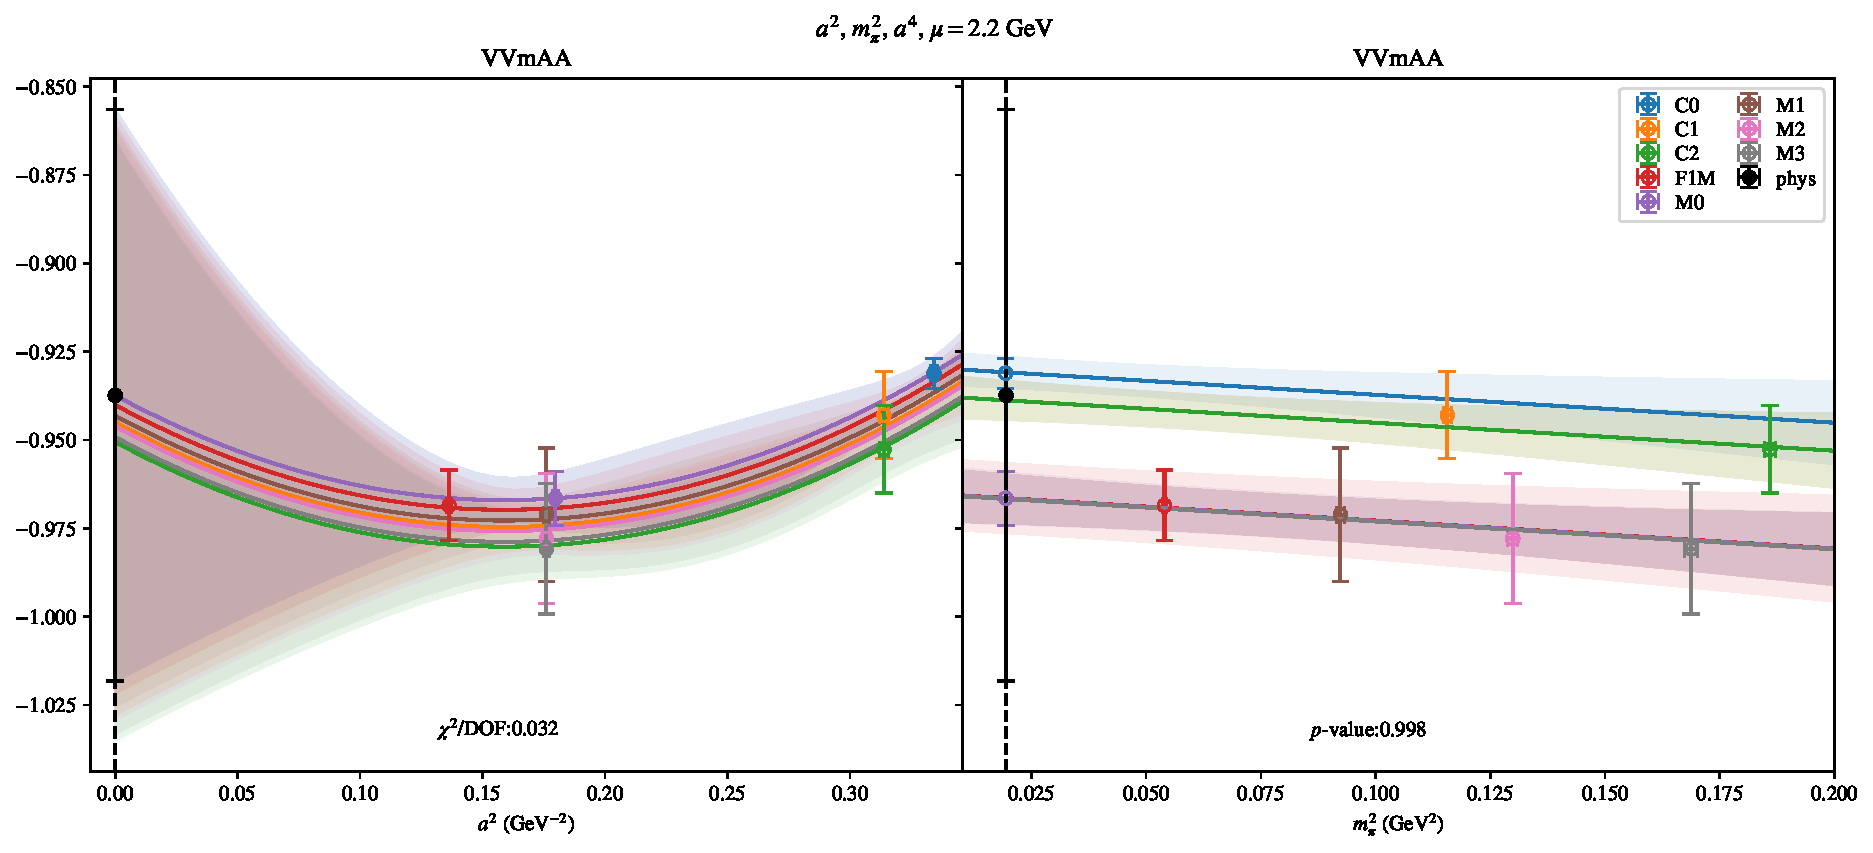
\includepdf[link, pages=-]{VVmAA/NPR/bag_a2a4m2_22.pdf}
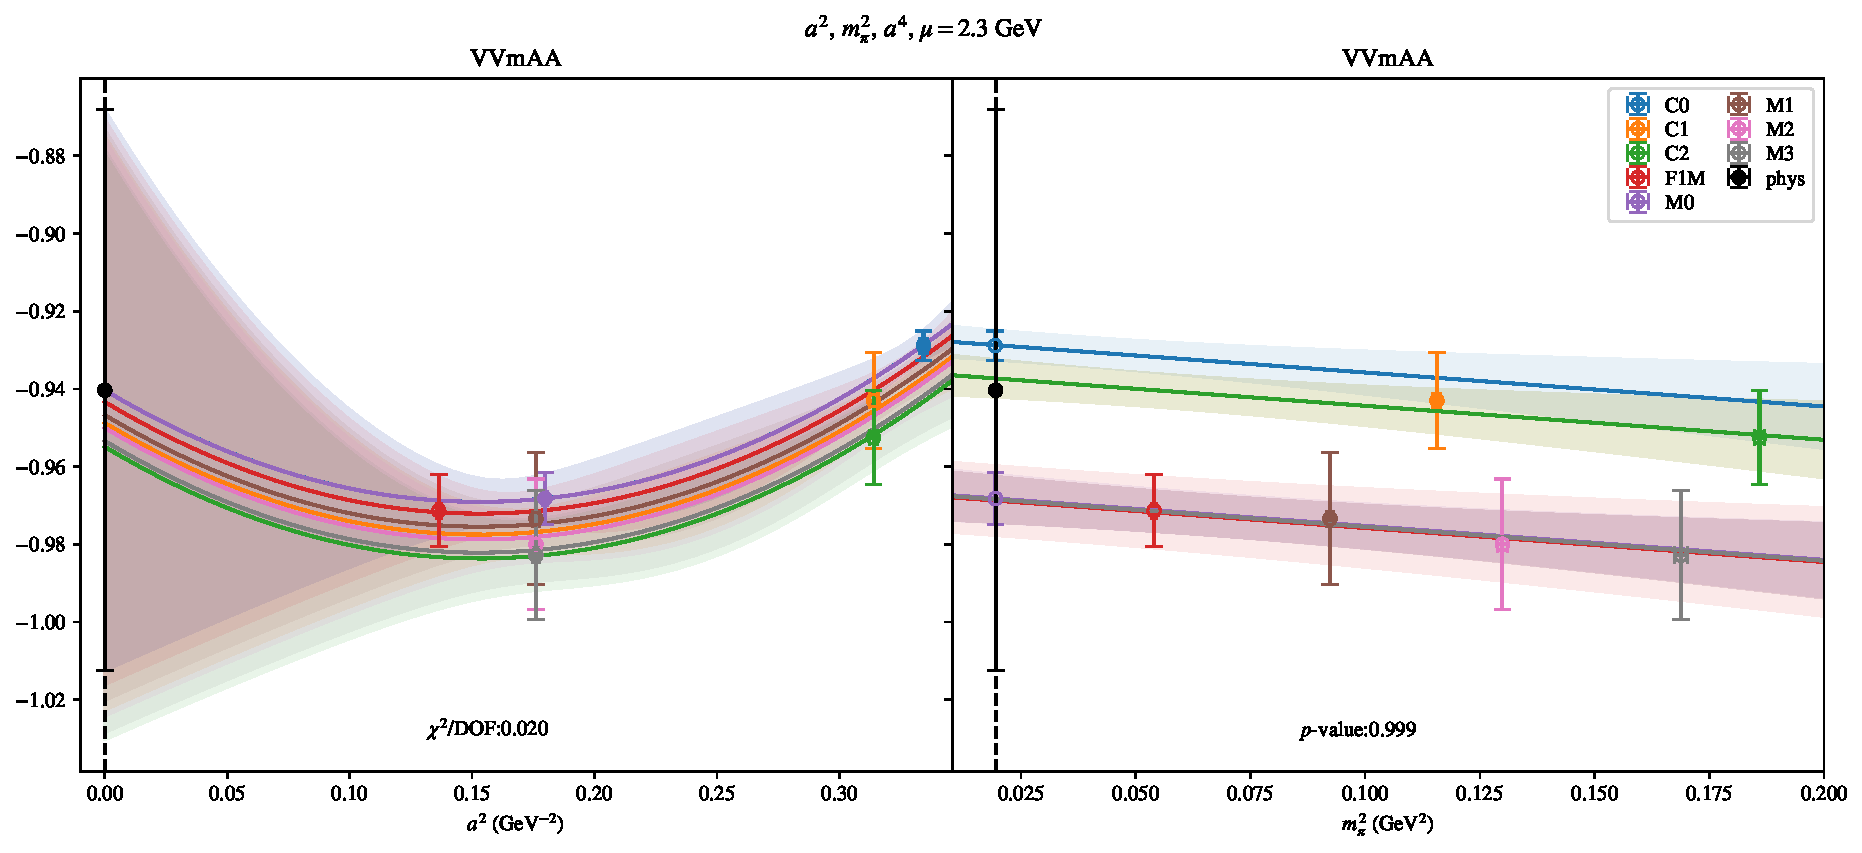
\includepdf[link, pages=-]{VVmAA/NPR/bag_a2a4m2_23.pdf}
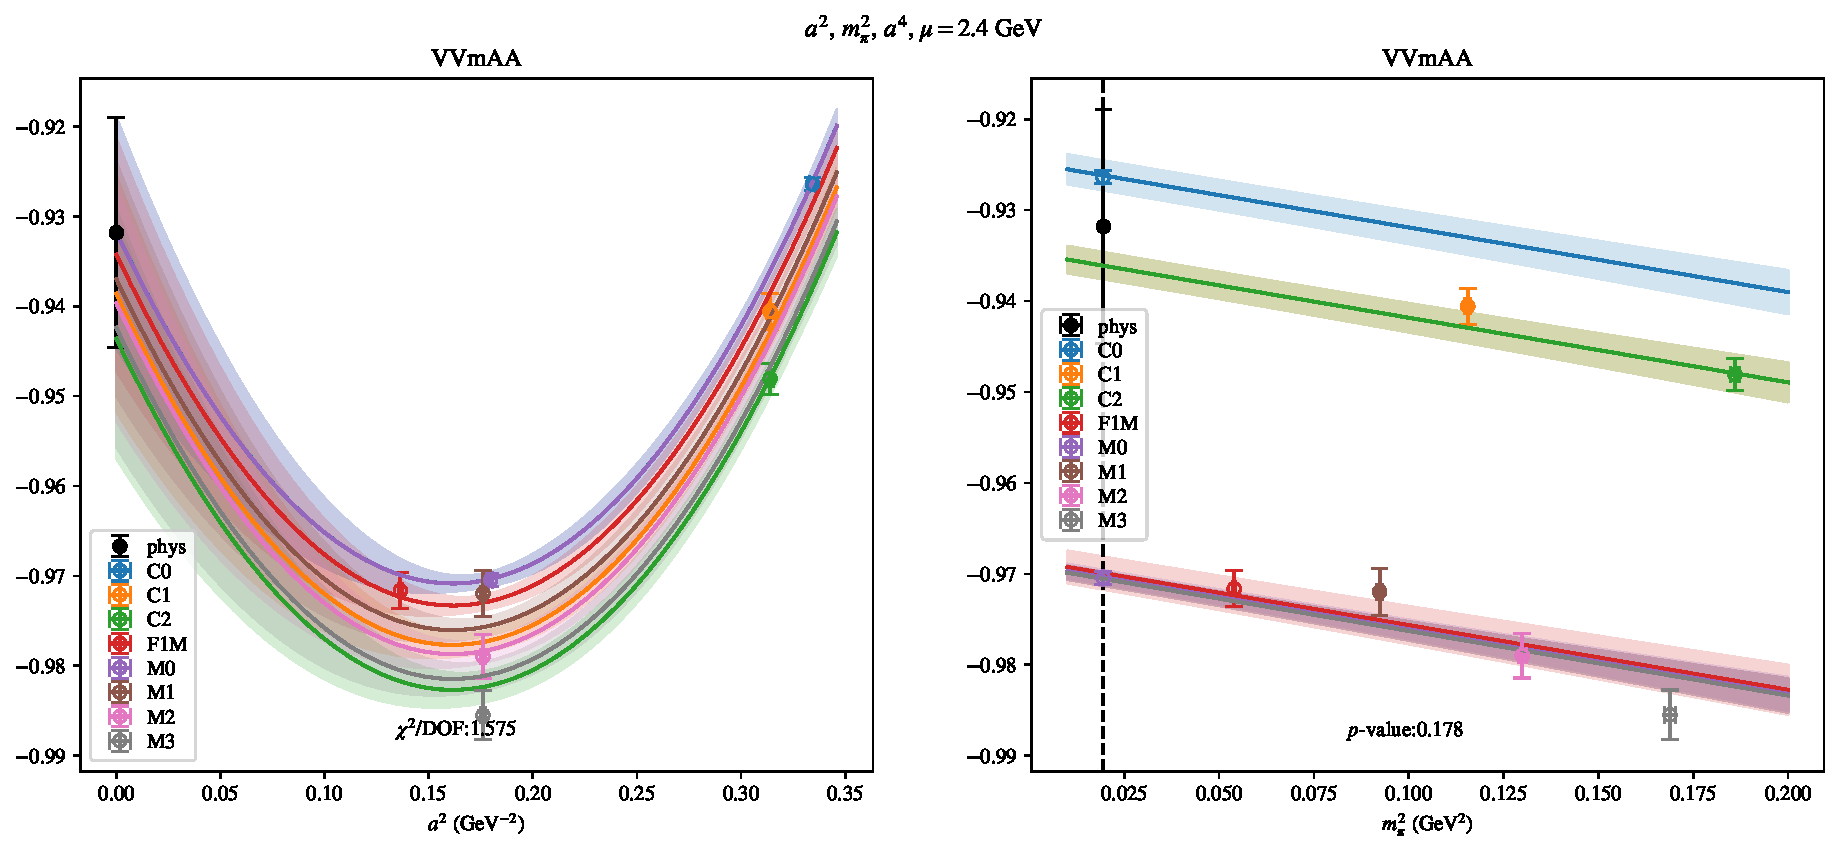
\includepdf[link, pages=-]{VVmAA/NPR/bag_a2a4m2_24.pdf}
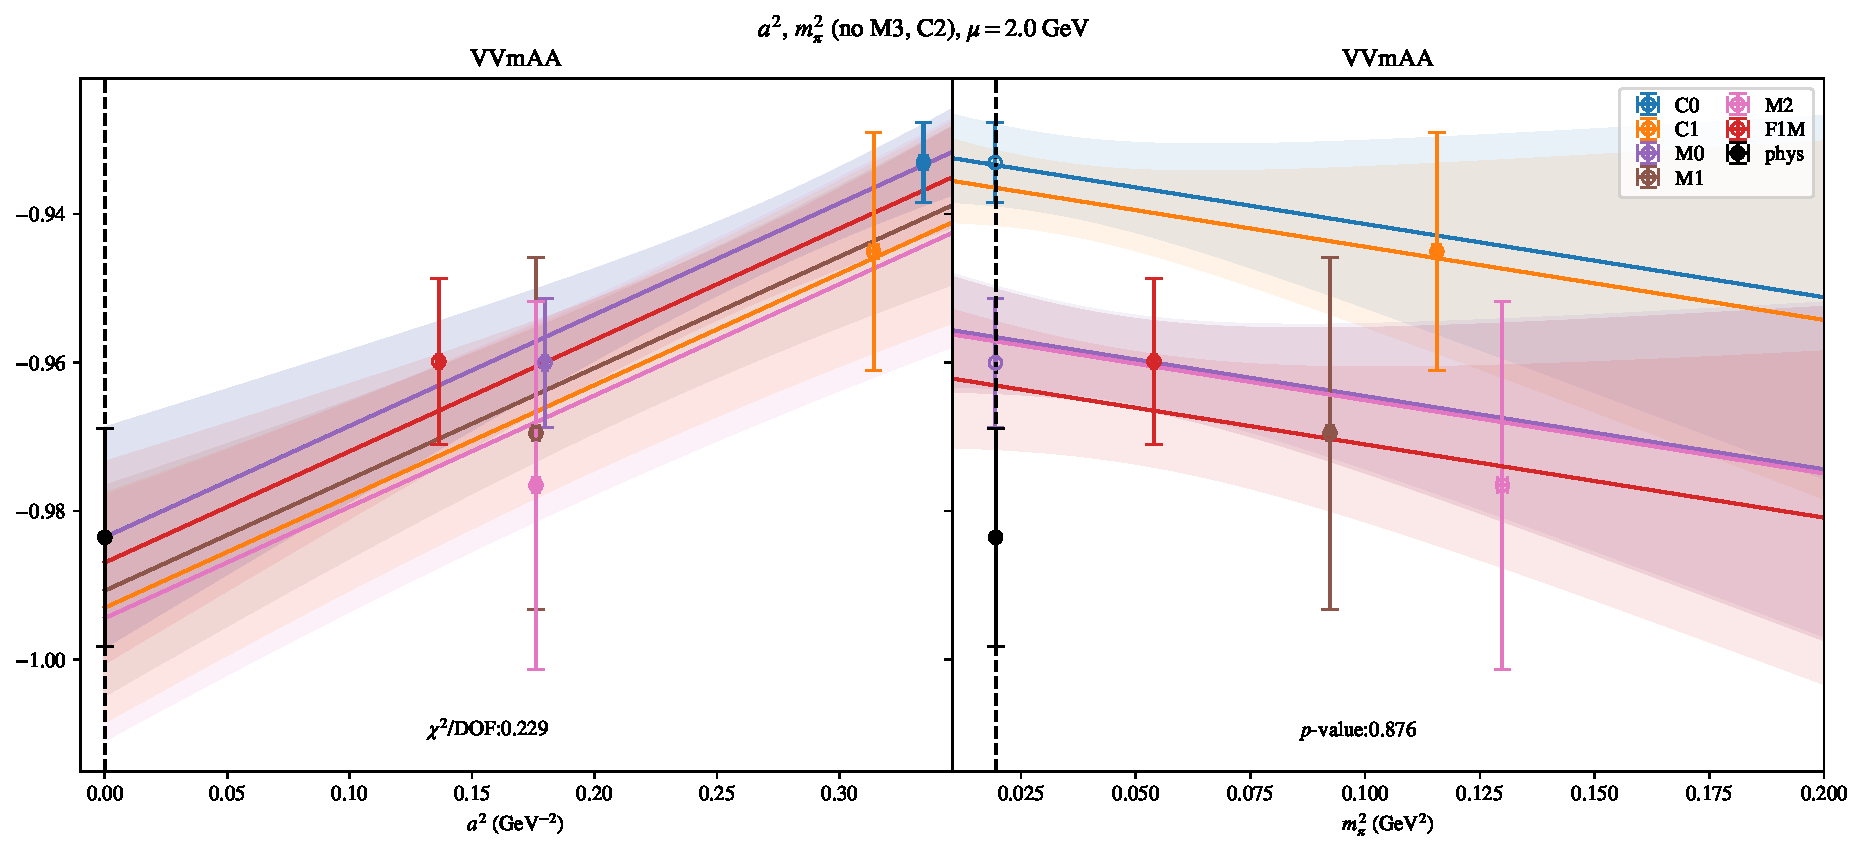
\includepdf[link, pages=-]{VVmAA/NPR/bag_a2m2mcut_20.pdf}
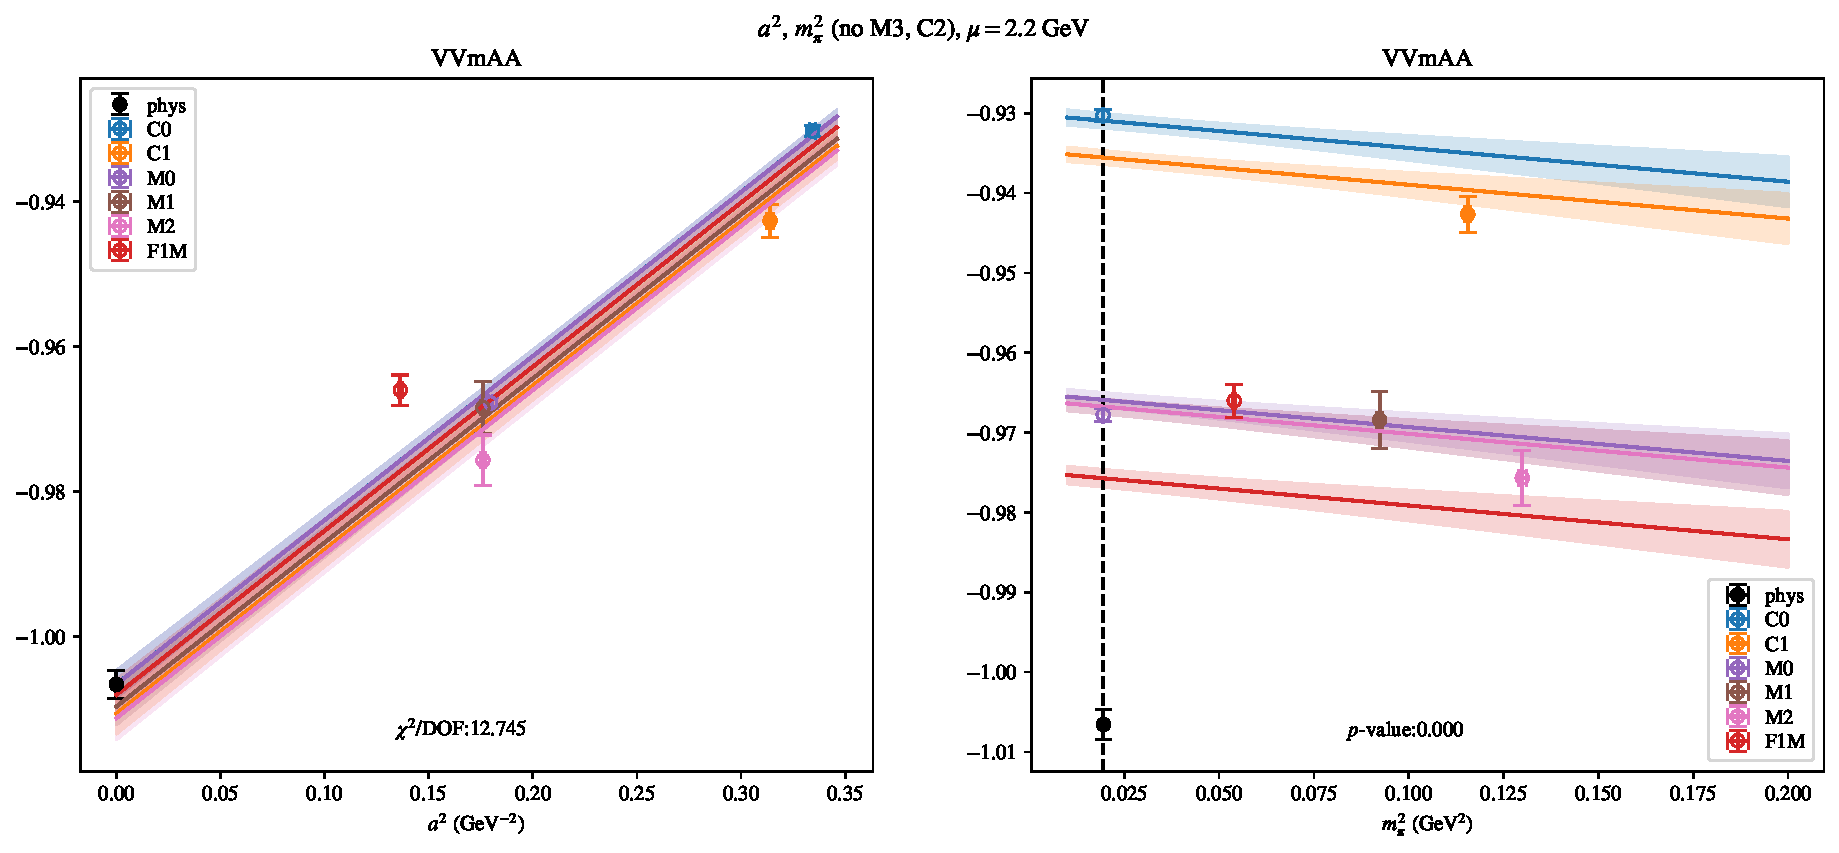
\includepdf[link, pages=-]{VVmAA/NPR/bag_a2m2mcut_22.pdf}
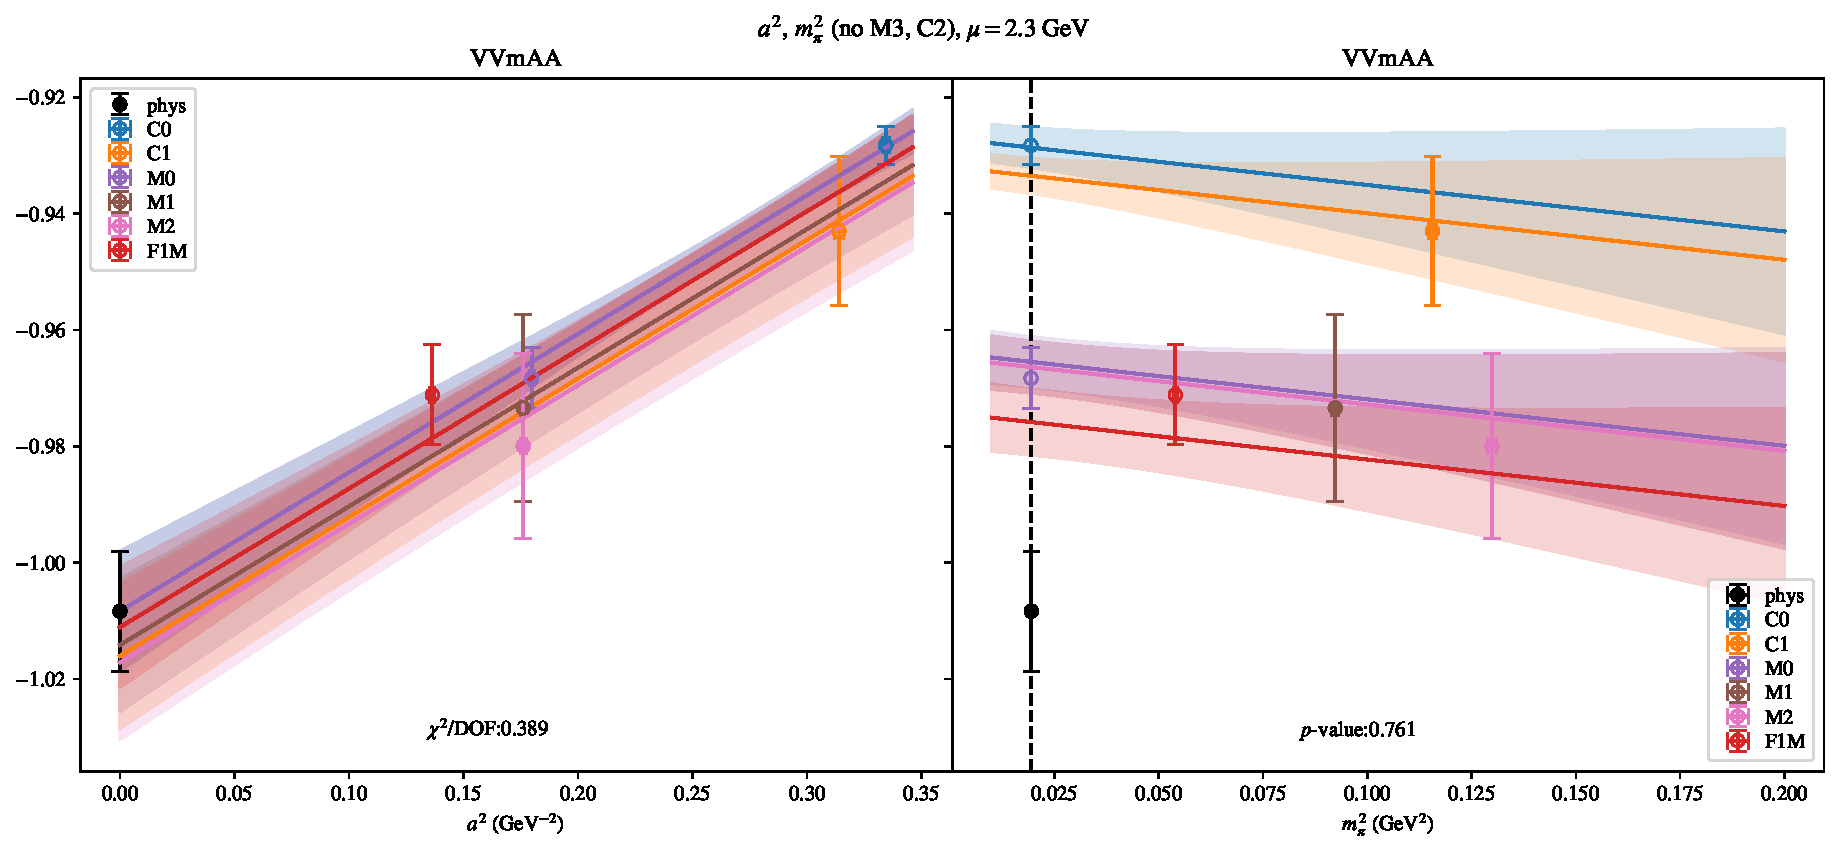
\includepdf[link, pages=-]{VVmAA/NPR/bag_a2m2mcut_23.pdf}
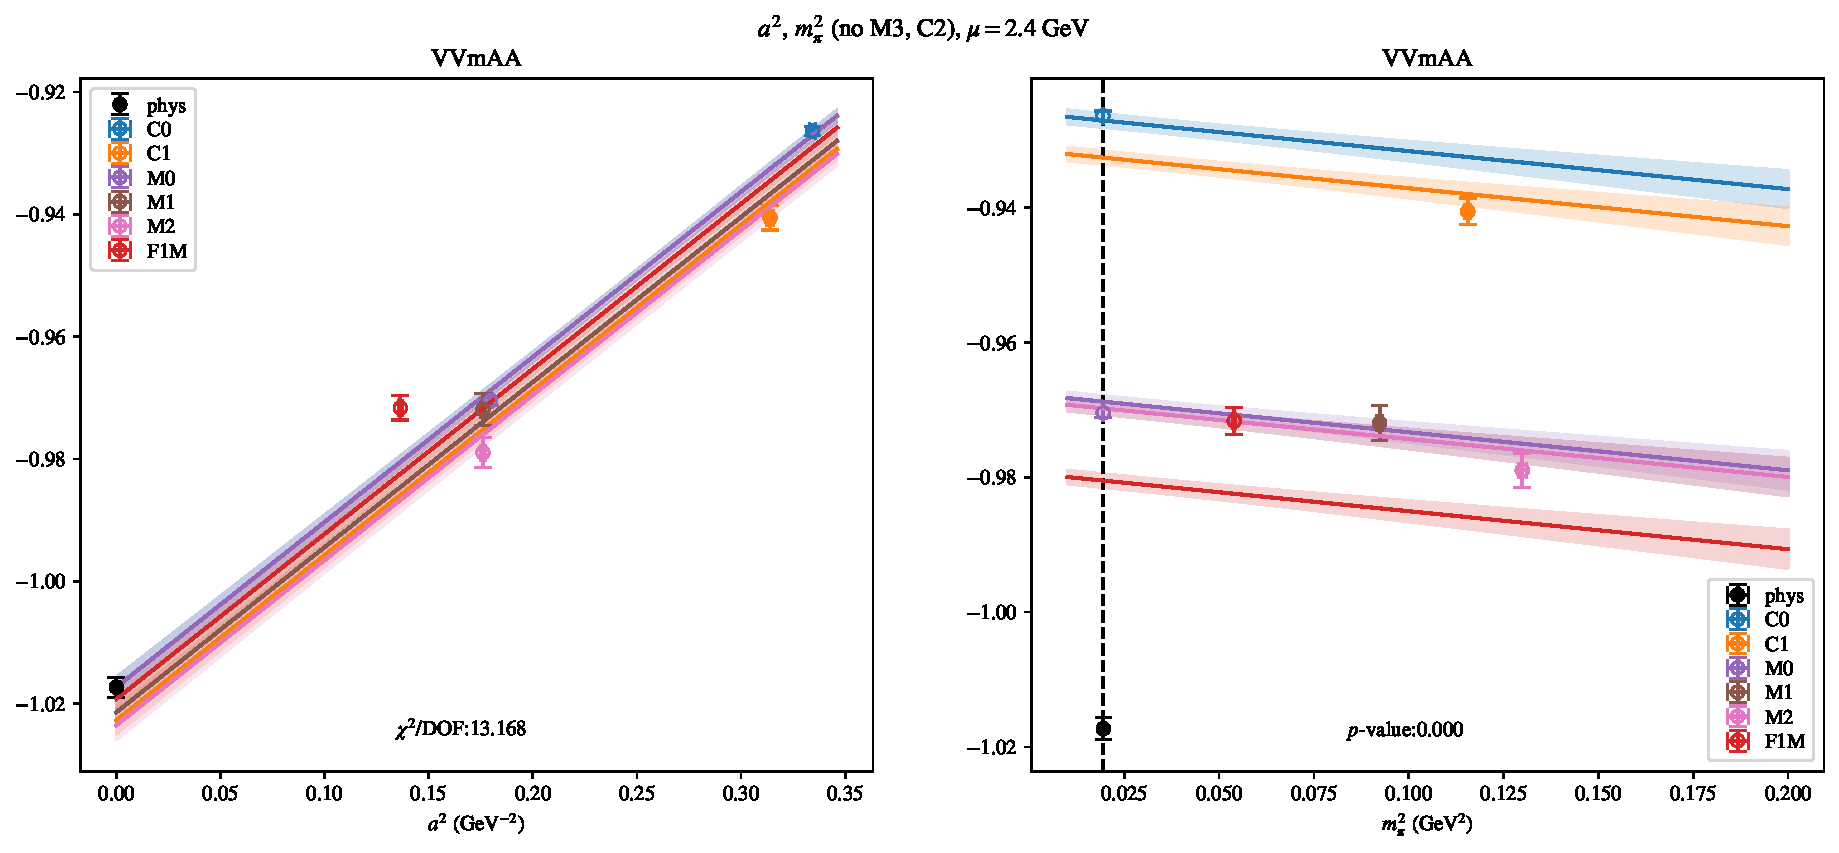
\includepdf[link, pages=-]{VVmAA/NPR/bag_a2m2mcut_24.pdf}
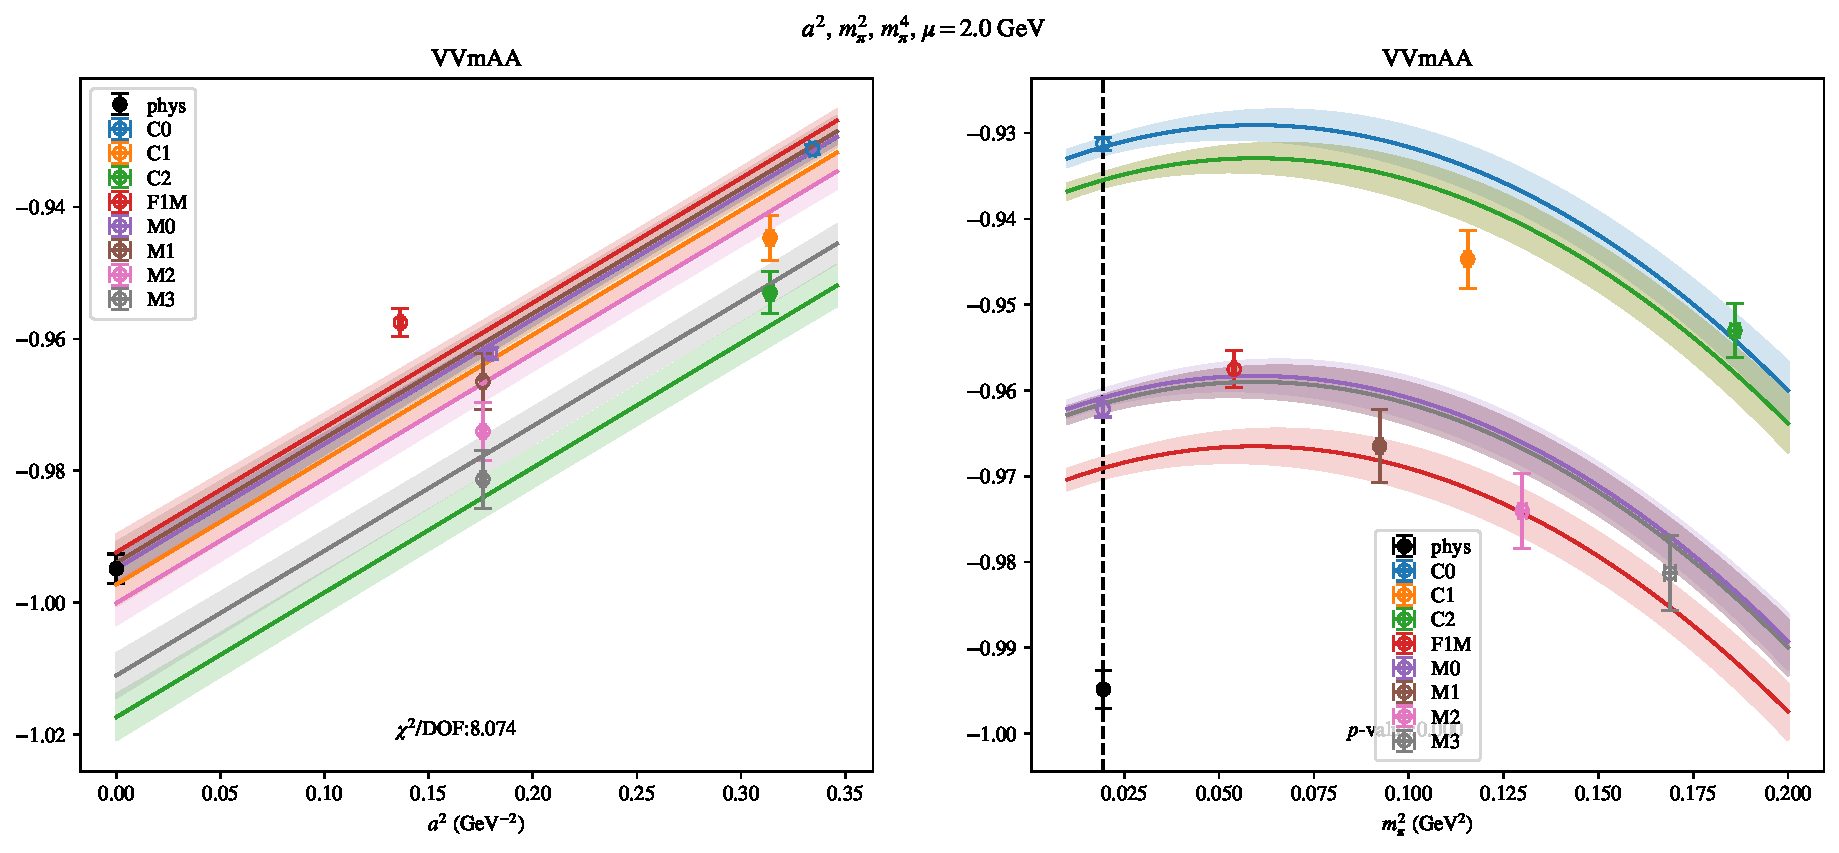
\includepdf[link, pages=-]{VVmAA/NPR/bag_a2m2m4_20.pdf}
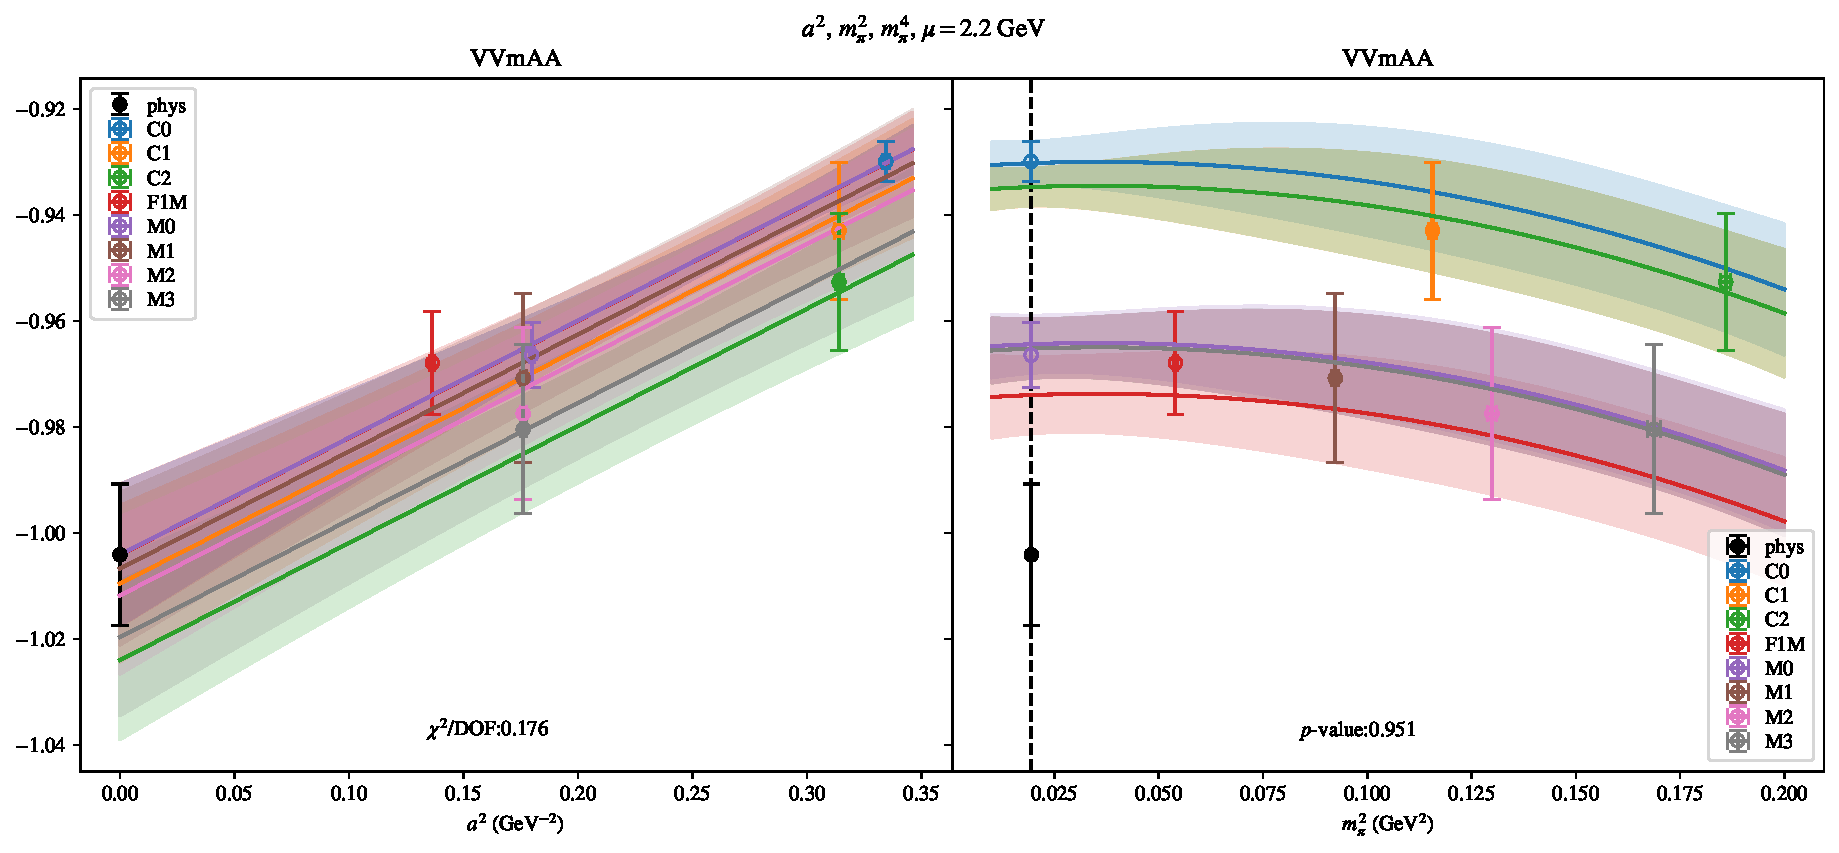
\includepdf[link, pages=-]{VVmAA/NPR/bag_a2m2m4_22.pdf}
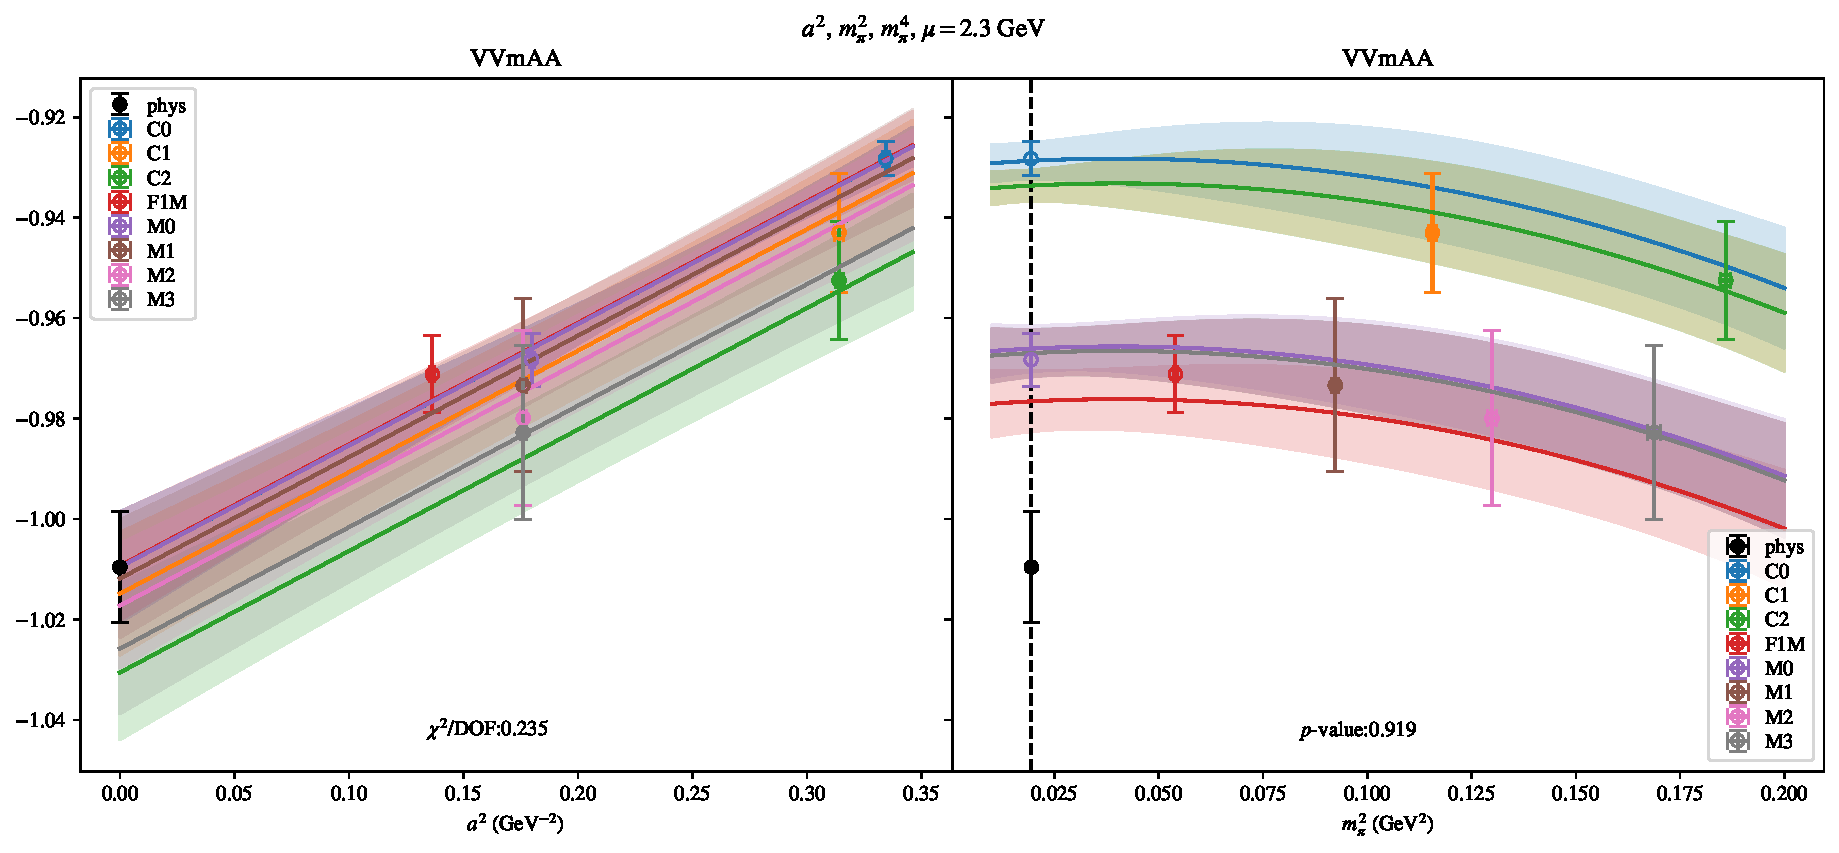
\includepdf[link, pages=-]{VVmAA/NPR/bag_a2m2m4_23.pdf}
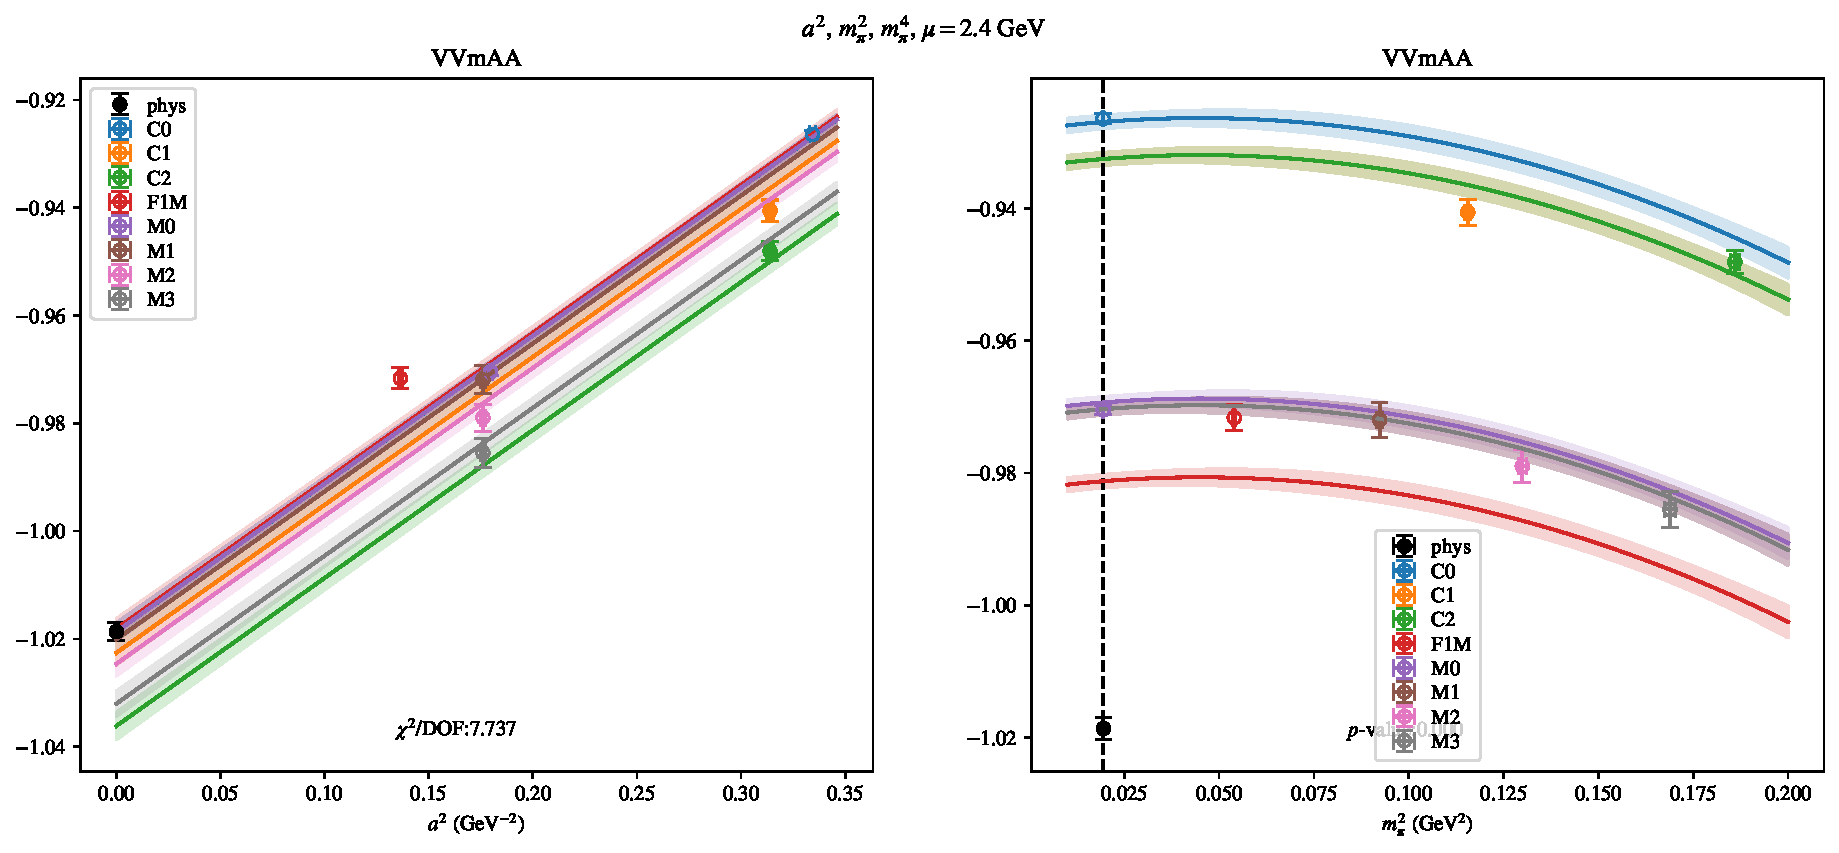
\includepdf[link, pages=-]{VVmAA/NPR/bag_a2m2m4_24.pdf}
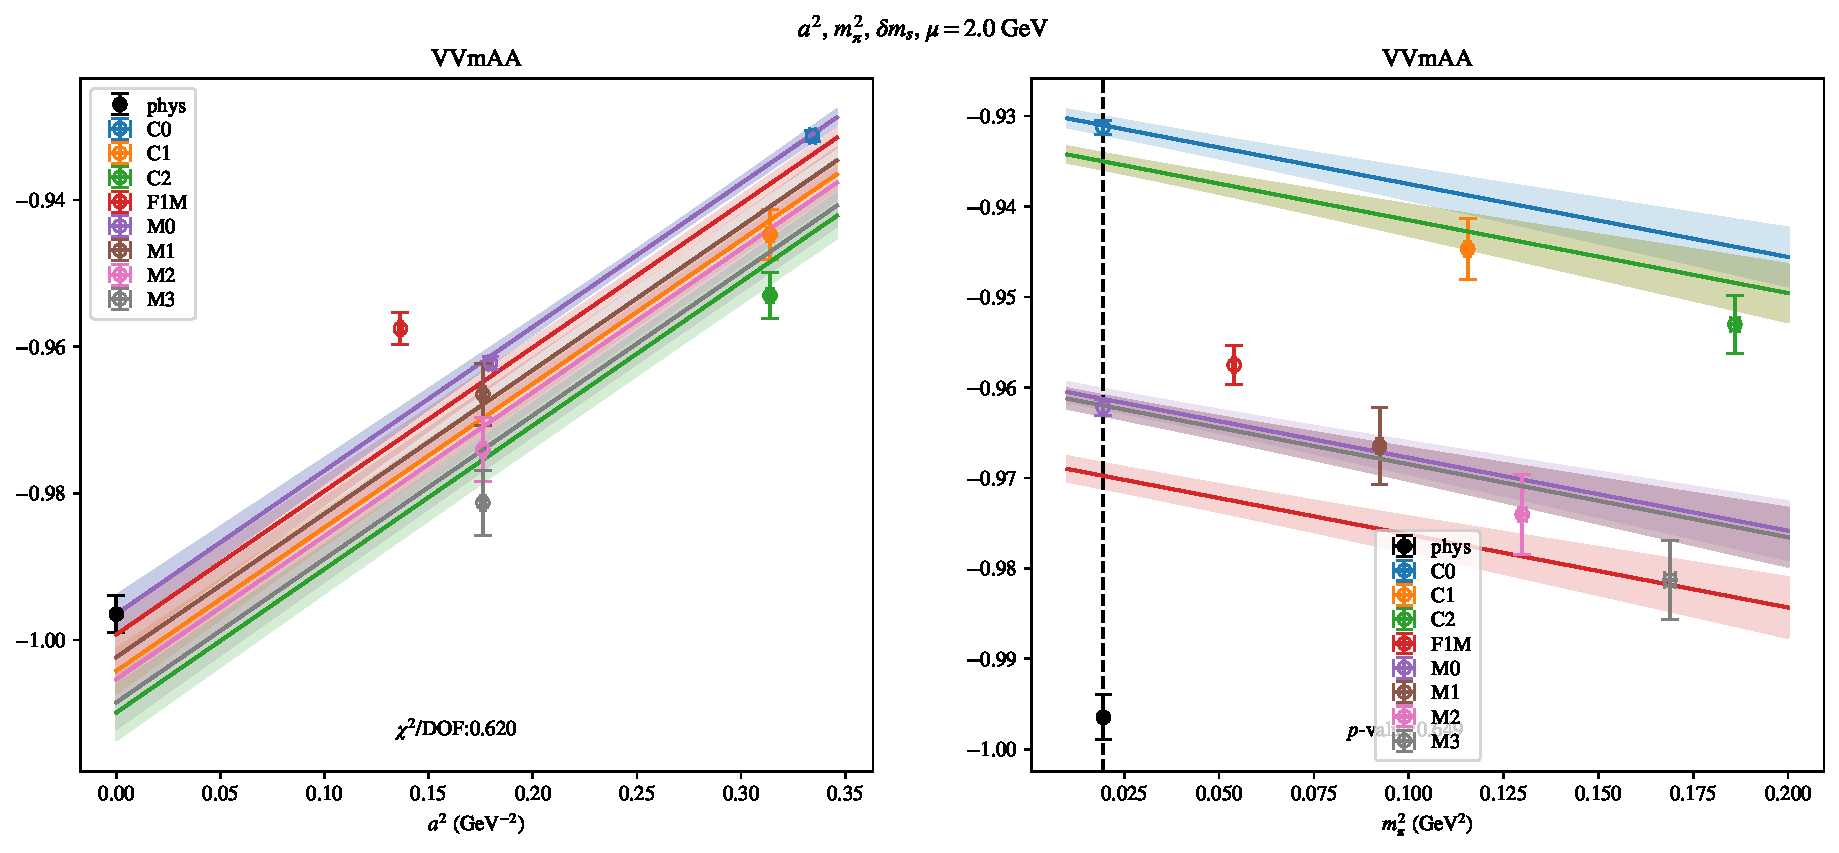
\includepdf[link, pages=-]{VVmAA/NPR/bag_a2m2delm_20.pdf}
\includepdf[link, pages=-]{VVmAA/NPR/bag_a2m2delm_22.pdf}
\includepdf[link, pages=-]{VVmAA/NPR/bag_a2m2delm_23.pdf}
\includepdf[link, pages=-]{VVmAA/NPR/bag_a2m2delm_24.pdf}
\clearpage
\section{$\mathcal{B}_3$}
\begin{table}[h!]
\begin{center}
\begin{tabular}{|c|c|c|c|c|c|c|}
\hline
$\mu$ (GeV) & $a^2$, $m_\pi^2$& $a^2$, $m_\pi^2$ (no C)& $a^2$, $m_\pi^2$, $a^4$& $a^2$, $m_\pi^2$ (no M3, C2)& $a^2$, $m_\pi^2$, $m_\pi^4$& $a^2$, $m_\pi^2$, $\delta m_s$\\
\hline
2.0& \hyperlink{SSmPP/NPR/bag_a2m2_20.pdf.1}{\textbf{1.7939(32)}: 9.144 (0.0)} & \hyperlink{SSmPP/NPR/bag_a2m2noC_20.pdf.1}{\textbf{1.706(13)}: 0.211 (0.81)} & \hyperlink{SSmPP/NPR/bag_a2a4m2_20.pdf.1}{\textbf{1.647(23)}: 0.862 (0.486)} & \hyperlink{SSmPP/NPR/bag_a2m2mcut_20.pdf.1}{\textbf{1.7948(36)}: 14.984 (0.0)} & \hyperlink{SSmPP/NPR/bag_a2m2m4_20.pdf.1}{\textbf{1.7979(37)}: 9.74 (0.0)} & \hyperlink{SSmPP/NPR/bag_a2m2delm_20.pdf.1}{\textbf{1.7932(31)}: 5.114 (0.0)}\\
2.2& \hyperlink{SSmPP/NPR/bag_a2m2_22.pdf.1}{\textbf{1.7991(31)}: 8.229 (0.0)} & \hyperlink{SSmPP/NPR/bag_a2m2noC_22.pdf.1}{\textbf{1.720(13)}: 0.184 (0.832)} & \hyperlink{SSmPP/NPR/bag_a2a4m2_22.pdf.1}{\textbf{1.666(22)}: 1.054 (0.378)} & \hyperlink{SSmPP/NPR/bag_a2m2mcut_22.pdf.1}{\textbf{1.8005(34)}: 13.122 (0.0)} & \hyperlink{SSmPP/NPR/bag_a2m2m4_22.pdf.1}{\textbf{1.8036(35)}: 8.188 (0.0)} & \hyperlink{SSmPP/NPR/bag_a2m2delm_22.pdf.1}{\textbf{1.7992(30)}: 6.059 (0.0)}\\
2.3& \hyperlink{SSmPP/NPR/bag_a2m2_23.pdf.1}{\textbf{1.8017(30)}: 7.647 (0.0)} & \hyperlink{SSmPP/NPR/bag_a2m2noC_23.pdf.1}{\textbf{1.725(13)}: 0.2 (0.819)} & \hyperlink{SSmPP/NPR/bag_a2a4m2_23.pdf.1}{\textbf{1.672(22)}: 0.815 (0.515)} & \hyperlink{SSmPP/NPR/bag_a2m2mcut_23.pdf.1}{\textbf{1.8028(34)}: 12.247 (0.0)} & \hyperlink{SSmPP/NPR/bag_a2m2m4_23.pdf.1}{\textbf{1.8057(34)}: 7.999 (0.0)} & \hyperlink{SSmPP/NPR/bag_a2m2delm_23.pdf.1}{\textbf{1.8014(30)}: 5.377 (0.0)}\\
2.4& \hyperlink{SSmPP/NPR/bag_a2m2_24.pdf.1}{\textbf{1.8035(30)}: 7.113 (0.0)} & \hyperlink{SSmPP/NPR/bag_a2m2noC_24.pdf.1}{\textbf{1.730(13)}: 0.192 (0.825)} & \hyperlink{SSmPP/NPR/bag_a2a4m2_24.pdf.1}{\textbf{1.678(22)}: 0.761 (0.55)} & \hyperlink{SSmPP/NPR/bag_a2m2mcut_24.pdf.1}{\textbf{1.8043(34)}: 11.59 (0.0)} & \hyperlink{SSmPP/NPR/bag_a2m2m4_24.pdf.1}{\textbf{1.8071(34)}: 7.554 (0.0)} & \hyperlink{SSmPP/NPR/bag_a2m2delm_24.pdf.1}{\textbf{1.8031(30)}: 5.043 (0.0)}\\
\hline
\end{tabular}
\caption{Physical point value from chiral and continuum extrapolation at renormalisation scale $\mu$. Entries are \textbf{value(error)}: $\chi^2/\text{DOF}$ ($p$-value).}
\end{center}
\end{table}
\begin{table}[h!]
\begin{center}
\begin{tabular}{|c c|c|c|c|c|c|c|}
\hline
$\mu$ (GeV) &  & $a^2$, $m_\pi^2$& $a^2$, $m_\pi^2$ (no C)& $a^2$, $m_\pi^2$, $a^4$& $a^2$, $m_\pi^2$ (no M3, C2)& $a^2$, $m_\pi^2$, $m_\pi^4$& $a^2$, $m_\pi^2$, $\delta m_s$\\
\hline
\multirow{3}{0.5in}{2.0} & $\alpha$ & 0.142(11)& 0.669(81)& 1.49(21)& 0.139(12)& 0.130(13)& 0.137(11)\\
 & $\beta$ & -0.00150(24)& -0.00171(57)& -0.00216(29)& -0.00176(43)& -0.0048(13)& -0.00403(59)\\
 & $\gamma$ &  &  & -2.74(43)&  & 0.00030(11)& 0.100(20)\\
\hline
\multirow{3}{0.5in}{2.2} & $\alpha$ & 0.153(11)& 0.631(77)& 1.38(20)& 0.149(12)& 0.140(12)& 0.147(11)\\
 & $\beta$ & -0.00094(23)& -0.00134(52)& -0.00158(27)& -0.00143(40)& -0.0044(12)& -0.00291(53)\\
 & $\gamma$ &  &  & -2.50(42)&  & 0.00032(10)& 0.078(18)\\
\hline
\multirow{3}{0.5in}{2.3} & $\alpha$ & 0.155(11)& 0.616(78)& 1.35(20)& 0.152(12)& 0.143(12)& 0.150(11)\\
 & $\beta$ & -0.00084(22)& -0.00124(51)& -0.00147(26)& -0.00124(39)& -0.0039(11)& -0.00276(54)\\
 & $\gamma$ &  &  & -2.43(42)&  & 0.00028(10)& 0.075(18)\\
\hline
\multirow{3}{0.5in}{2.4} & $\alpha$ & 0.157(11)& 0.602(77)& 1.31(20)& 0.154(12)& 0.146(12)& 0.152(11)\\
 & $\beta$ & -0.00076(22)& -0.00113(50)& -0.00137(26)& -0.00106(38)& -0.0035(11)& -0.00261(53)\\
 & $\gamma$ &  &  & -2.34(42)&  & 0.00025(10)& 0.072(18)\\
\hline
\end{tabular}
\caption{Fit values of coefficients in $Q = Q_{phys} + \mathbf{\alpha} a^2 + \mathbf{\beta}\left(\frac{m_\pi^2}{f_\pi^2}-\frac{m_{\pi,PDG}^2}{f_\pi^2}\right) + \gamma(\ldots)$}
\end{center}
\end{table}
\includepdf[link, pages=-]{SSmPP/NPR/bag_a2m2_20.pdf}
\includepdf[link, pages=-]{SSmPP/NPR/bag_a2m2_22.pdf}
\includepdf[link, pages=-]{SSmPP/NPR/bag_a2m2_23.pdf}
\includepdf[link, pages=-]{SSmPP/NPR/bag_a2m2_24.pdf}
\includepdf[link, pages=-]{SSmPP/NPR/bag_a2m2noC_20.pdf}
\includepdf[link, pages=-]{SSmPP/NPR/bag_a2m2noC_22.pdf}
\includepdf[link, pages=-]{SSmPP/NPR/bag_a2m2noC_23.pdf}
\includepdf[link, pages=-]{SSmPP/NPR/bag_a2m2noC_24.pdf}
\includepdf[link, pages=-]{SSmPP/NPR/bag_a2a4m2_20.pdf}
\includepdf[link, pages=-]{SSmPP/NPR/bag_a2a4m2_22.pdf}
\includepdf[link, pages=-]{SSmPP/NPR/bag_a2a4m2_23.pdf}
\includepdf[link, pages=-]{SSmPP/NPR/bag_a2a4m2_24.pdf}
\includepdf[link, pages=-]{SSmPP/NPR/bag_a2m2mcut_20.pdf}
\includepdf[link, pages=-]{SSmPP/NPR/bag_a2m2mcut_22.pdf}
\includepdf[link, pages=-]{SSmPP/NPR/bag_a2m2mcut_23.pdf}
\includepdf[link, pages=-]{SSmPP/NPR/bag_a2m2mcut_24.pdf}
\includepdf[link, pages=-]{SSmPP/NPR/bag_a2m2m4_20.pdf}
\includepdf[link, pages=-]{SSmPP/NPR/bag_a2m2m4_22.pdf}
\includepdf[link, pages=-]{SSmPP/NPR/bag_a2m2m4_23.pdf}
\includepdf[link, pages=-]{SSmPP/NPR/bag_a2m2m4_24.pdf}
\includepdf[link, pages=-]{SSmPP/NPR/bag_a2m2delm_20.pdf}
\includepdf[link, pages=-]{SSmPP/NPR/bag_a2m2delm_22.pdf}
\includepdf[link, pages=-]{SSmPP/NPR/bag_a2m2delm_23.pdf}
\includepdf[link, pages=-]{SSmPP/NPR/bag_a2m2delm_24.pdf}
\clearpage
\section{$\mathcal{B}_4$}
\begin{table}[h!]
\begin{center}
\begin{tabular}{|c|c|c|c|c|c|c|}
\hline
$\mu$ (GeV) & $a^2$, $m_\pi^2$& $a^2$, $m_\pi^2$ (no C)& $a^2$, $m_\pi^2$, $a^4$& $a^2$, $m_\pi^2$ (no M3, C2)& $a^2$, $m_\pi^2$, $m_\pi^4$& $a^2$, $m_\pi^2$, $\delta m_s$\\
\hline
2.0& \hyperlink{SSpPP/NPR/bag_a2m2_20.pdf.1}{\textbf{-0.9261(19)}: 3.536 (0.003)} & \hyperlink{SSpPP/NPR/bag_a2m2noC_20.pdf.1}{\textbf{-0.9460(80)}: 2.15 (0.116)} & \hyperlink{SSpPP/NPR/bag_a2a4m2_20.pdf.1}{\textbf{-0.948(12)}: 3.802 (0.004)} & \hyperlink{SSpPP/NPR/bag_a2m2mcut_20.pdf.1}{\textbf{-0.9253(20)}: 3.748 (0.01)} & \hyperlink{SSpPP/NPR/bag_a2m2m4_20.pdf.1}{\textbf{-0.9233(21)}: 2.329 (0.054)} & \hyperlink{SSpPP/NPR/bag_a2m2delm_20.pdf.1}{\textbf{-0.9260(19)}: 4.508 (0.001)}\\
2.2& \hyperlink{SSpPP/NPR/bag_a2m2_22.pdf.1}{\textbf{-0.9064(18)}: 4.659 (0.0)} & \hyperlink{SSpPP/NPR/bag_a2m2noC_22.pdf.1}{\textbf{-0.9300(74)}: 1.662 (0.19)} & \hyperlink{SSpPP/NPR/bag_a2a4m2_22.pdf.1}{\textbf{-0.931(12)}: 4.87 (0.001)} & \hyperlink{SSpPP/NPR/bag_a2m2mcut_22.pdf.1}{\textbf{-0.9062(20)}: 5.25 (0.001)} & \hyperlink{SSpPP/NPR/bag_a2m2m4_22.pdf.1}{\textbf{-0.9039(20)}: 3.903 (0.004)} & \hyperlink{SSpPP/NPR/bag_a2m2delm_22.pdf.1}{\textbf{-0.9064(18)}: 5.779 (0.0)}\\
2.3& \hyperlink{SSpPP/NPR/bag_a2m2_23.pdf.1}{\textbf{-0.8977(18)}: 5.355 (0.0)} & \hyperlink{SSpPP/NPR/bag_a2m2noC_23.pdf.1}{\textbf{-0.9227(73)}: 1.877 (0.153)} & \hyperlink{SSpPP/NPR/bag_a2a4m2_23.pdf.1}{\textbf{-0.924(11)}: 5.704 (0.0)} & \hyperlink{SSpPP/NPR/bag_a2m2mcut_23.pdf.1}{\textbf{-0.8975(19)}: 6.201 (0.0)} & \hyperlink{SSpPP/NPR/bag_a2m2m4_23.pdf.1}{\textbf{-0.8950(20)}: 4.512 (0.001)} & \hyperlink{SSpPP/NPR/bag_a2m2delm_23.pdf.1}{\textbf{-0.8978(17)}: 6.715 (0.0)}\\
2.4& \hyperlink{SSpPP/NPR/bag_a2m2_24.pdf.1}{\textbf{-0.8899(18)}: 5.792 (0.0)} & \hyperlink{SSpPP/NPR/bag_a2m2noC_24.pdf.1}{\textbf{-0.9154(72)}: 1.918 (0.147)} & \hyperlink{SSpPP/NPR/bag_a2a4m2_24.pdf.1}{\textbf{-0.917(11)}: 6.102 (0.0)} & \hyperlink{SSpPP/NPR/bag_a2m2mcut_24.pdf.1}{\textbf{-0.8897(19)}: 7.05 (0.0)} & \hyperlink{SSpPP/NPR/bag_a2m2m4_24.pdf.1}{\textbf{-0.8873(20)}: 4.908 (0.001)} & \hyperlink{SSpPP/NPR/bag_a2m2delm_24.pdf.1}{\textbf{-0.8900(17)}: 7.278 (0.0)}\\
\hline
\end{tabular}
\caption{Physical point value from chiral and continuum extrapolation at renormalisation scale $\mu$. Entries are \textbf{value(error)}: $\chi^2/\text{DOF}$ ($p$-value).}
\end{center}
\end{table}
\begin{table}[h!]
\begin{center}
\begin{tabular}{|c c|c|c|c|c|c|c|}
\hline
$\mu$ (GeV) &  & $a^2$, $m_\pi^2$& $a^2$, $m_\pi^2$ (no C)& $a^2$, $m_\pi^2$, $a^4$& $a^2$, $m_\pi^2$ (no M3, C2)& $a^2$, $m_\pi^2$, $m_\pi^4$& $a^2$, $m_\pi^2$, $\delta m_s$\\
\hline
\multirow{3}{0.5in}{2.0} & $\alpha$ & -0.3484(73)& -0.233(46)& -0.15(11)& -0.3503(78)& -0.3570(79)& -0.3488(74)\\
 & $\beta$ & -0.00626(16)& -0.00588(29)& -0.00634(16)& -0.00673(26)& -0.00864(82)& -0.00629(31)\\
 & $\gamma$ &  &  & -0.41(23)&  & 0.000218(74)& 0.001(11)\\
\hline
\multirow{3}{0.5in}{2.2} & $\alpha$ & -0.3830(71)& -0.248(43)& -0.16(11)& -0.3825(76)& -0.3907(76)& -0.3832(70)\\
 & $\beta$ & -0.00650(15)& -0.00596(26)& -0.00660(15)& -0.00690(24)& -0.00864(78)& -0.00662(29)\\
 & $\gamma$ &  &  & -0.46(22)&  & 0.000196(70)& 0.005(10)\\
\hline
\multirow{3}{0.5in}{2.3} & $\alpha$ & -0.3985(69)& -0.256(42)& -0.16(10)& -0.3983(74)& -0.4069(75)& -0.3990(69)\\
 & $\beta$ & -0.00651(14)& -0.00599(26)& -0.00662(15)& -0.00693(24)& -0.00874(75)& -0.00663(29)\\
 & $\gamma$ &  &  & -0.49(22)&  & 0.000204(67)& 0.005(10)\\
\hline
\multirow{3}{0.5in}{2.4} & $\alpha$ & -0.4127(69)& -0.267(42)& -0.17(10)& -0.4124(75)& -0.4207(75)& -0.4130(69)\\
 & $\beta$ & -0.00653(14)& -0.00600(25)& -0.00664(15)& -0.00691(23)& -0.00877(74)& -0.00668(29)\\
 & $\gamma$ &  &  & -0.50(22)&  & 0.000204(66)& 0.006(10)\\
\hline
\end{tabular}
\caption{Fit values of coefficients in $Q = Q_{phys} + \mathbf{\alpha} a^2 + \mathbf{\beta}\left(\frac{m_\pi^2}{f_\pi^2}-\frac{m_{\pi,PDG}^2}{f_\pi^2}\right) + \gamma(\ldots)$}
\end{center}
\end{table}
\includepdf[link, pages=-]{SSpPP/NPR/bag_a2m2_20.pdf}
\includepdf[link, pages=-]{SSpPP/NPR/bag_a2m2_22.pdf}
\includepdf[link, pages=-]{SSpPP/NPR/bag_a2m2_23.pdf}
\includepdf[link, pages=-]{SSpPP/NPR/bag_a2m2_24.pdf}
\includepdf[link, pages=-]{SSpPP/NPR/bag_a2m2noC_20.pdf}
\includepdf[link, pages=-]{SSpPP/NPR/bag_a2m2noC_22.pdf}
\includepdf[link, pages=-]{SSpPP/NPR/bag_a2m2noC_23.pdf}
\includepdf[link, pages=-]{SSpPP/NPR/bag_a2m2noC_24.pdf}
\includepdf[link, pages=-]{SSpPP/NPR/bag_a2a4m2_20.pdf}
\includepdf[link, pages=-]{SSpPP/NPR/bag_a2a4m2_22.pdf}
\includepdf[link, pages=-]{SSpPP/NPR/bag_a2a4m2_23.pdf}
\includepdf[link, pages=-]{SSpPP/NPR/bag_a2a4m2_24.pdf}
\includepdf[link, pages=-]{SSpPP/NPR/bag_a2m2mcut_20.pdf}
\includepdf[link, pages=-]{SSpPP/NPR/bag_a2m2mcut_22.pdf}
\includepdf[link, pages=-]{SSpPP/NPR/bag_a2m2mcut_23.pdf}
\includepdf[link, pages=-]{SSpPP/NPR/bag_a2m2mcut_24.pdf}
\includepdf[link, pages=-]{SSpPP/NPR/bag_a2m2m4_20.pdf}
\includepdf[link, pages=-]{SSpPP/NPR/bag_a2m2m4_22.pdf}
\includepdf[link, pages=-]{SSpPP/NPR/bag_a2m2m4_23.pdf}
\includepdf[link, pages=-]{SSpPP/NPR/bag_a2m2m4_24.pdf}
\includepdf[link, pages=-]{SSpPP/NPR/bag_a2m2delm_20.pdf}
\includepdf[link, pages=-]{SSpPP/NPR/bag_a2m2delm_22.pdf}
\includepdf[link, pages=-]{SSpPP/NPR/bag_a2m2delm_23.pdf}
\includepdf[link, pages=-]{SSpPP/NPR/bag_a2m2delm_24.pdf}
\clearpage
\section{$\mathcal{B}_5$}
\begin{table}[h!]
\begin{center}
\begin{tabular}{|c|c|c|c|c|c|c|}
\hline
$\mu$ (GeV) & $a^2$, $m_\pi^2$& $a^2$, $m_\pi^2$ (no C)& $a^2$, $m_\pi^2$, $a^4$& $a^2$, $m_\pi^2$ (no M3, C2)& $a^2$, $m_\pi^2$, $m_\pi^4$& $a^2$, $m_\pi^2$, $\delta m_s$\\
\hline
2.0& \hyperlink{TT/NPR/bag_a2m2_20.pdf.1}{\textbf{-0.3625(43)}: 0.057 (0.998)} & \hyperlink{TT/NPR/bag_a2m2noC_20.pdf.1}{\textbf{-0.369(18)}: 0.023 (0.977)} & \hyperlink{TT/NPR/bag_a2a4m2_20.pdf.1}{\textbf{-0.369(32)}: 0.057 (0.994)} & \hyperlink{TT/NPR/bag_a2m2mcut_20.pdf.1}{\textbf{-0.3623(48)}: 0.042 (0.988)} & \hyperlink{TT/NPR/bag_a2m2m4_20.pdf.1}{\textbf{-0.3616(46)}: 0.035 (0.998)} & \hyperlink{TT/NPR/bag_a2m2delm_20.pdf.1}{\textbf{-0.3624(42)}: 0.069 (0.991)}\\
2.2& \hyperlink{TT/NPR/bag_a2m2_22.pdf.1}{\textbf{-0.3597(36)}: 0.077 (0.996)} & \hyperlink{TT/NPR/bag_a2m2noC_22.pdf.1}{\textbf{-0.367(16)}: 0.013 (0.987)} & \hyperlink{TT/NPR/bag_a2a4m2_22.pdf.1}{\textbf{-0.367(28)}: 0.075 (0.99)} & \hyperlink{TT/NPR/bag_a2m2mcut_22.pdf.1}{\textbf{-0.3598(40)}: 0.086 (0.968)} & \hyperlink{TT/NPR/bag_a2m2m4_22.pdf.1}{\textbf{-0.3590(42)}: 0.068 (0.992)} & \hyperlink{TT/NPR/bag_a2m2delm_22.pdf.1}{\textbf{-0.3597(38)}: 0.097 (0.984)}\\
2.3& \hyperlink{TT/NPR/bag_a2m2_23.pdf.1}{\textbf{-0.3587(35)}: 0.1 (0.992)} & \hyperlink{TT/NPR/bag_a2m2noC_23.pdf.1}{\textbf{-0.366(15)}: 0.026 (0.975)} & \hyperlink{TT/NPR/bag_a2a4m2_23.pdf.1}{\textbf{-0.365(25)}: 0.109 (0.98)} & \hyperlink{TT/NPR/bag_a2m2mcut_23.pdf.1}{\textbf{-0.3586(38)}: 0.098 (0.961)} & \hyperlink{TT/NPR/bag_a2m2m4_23.pdf.1}{\textbf{-0.3579(37)}: 0.062 (0.993)} & \hyperlink{TT/NPR/bag_a2m2delm_23.pdf.1}{\textbf{-0.3586(33)}: 0.125 (0.973)}\\
2.4& \hyperlink{TT/NPR/bag_a2m2_24.pdf.1}{\textbf{-0.3579(31)}: 0.121 (0.988)} & \hyperlink{TT/NPR/bag_a2m2noC_24.pdf.1}{\textbf{-0.365(13)}: 0.043 (0.958)} & \hyperlink{TT/NPR/bag_a2a4m2_24.pdf.1}{\textbf{-0.364(23)}: 0.142 (0.966)} & \hyperlink{TT/NPR/bag_a2m2mcut_24.pdf.1}{\textbf{-0.3575(34)}: 0.118 (0.949)} & \hyperlink{TT/NPR/bag_a2m2m4_24.pdf.1}{\textbf{-0.3569(33)}: 0.063 (0.993)} & \hyperlink{TT/NPR/bag_a2m2delm_24.pdf.1}{\textbf{-0.3578(30)}: 0.15 (0.963)}\\
\hline
\end{tabular}
\caption{Physical point value from chiral and continuum extrapolation at renormalisation scale $\mu$. Entries are \textbf{value(error)}: $\chi^2/\text{DOF}$ ($p$-value).}
\end{center}
\end{table}
\begin{table}[h!]
\begin{center}
\begin{tabular}{|c c|c|c|c|c|c|c|}
\hline
$\mu$ (GeV) &  & $a^2$, $m_\pi^2$& $a^2$, $m_\pi^2$ (no C)& $a^2$, $m_\pi^2$, $a^4$& $a^2$, $m_\pi^2$ (no M3, C2)& $a^2$, $m_\pi^2$, $m_\pi^4$& $a^2$, $m_\pi^2$, $\delta m_s$\\
\hline
\multirow{3}{0.5in}{2.0} & $\alpha$ & 0.013(15)& 0.05(11)& 0.08(29)& 0.013(16)& 0.010(15)& 0.013(14)\\
 & $\beta$ & -0.00223(29)& -0.00218(57)& -0.00228(32)& -0.00236(49)& -0.0028(14)& -0.00220(64)\\
 & $\gamma$ &  &  & -0.13(59)&  & 0.00005(12)& -0.001(23)\\
\hline
\multirow{3}{0.5in}{2.2} & $\alpha$ & 0.028(12)& 0.071(94)& 0.10(25)& 0.028(13)& 0.026(14)& 0.028(13)\\
 & $\beta$ & -0.00229(25)& -0.00220(47)& -0.00233(28)& -0.00237(41)& -0.0027(12)& -0.00229(56)\\
 & $\gamma$ &  &  & -0.14(52)&  & 0.00003(10)& 0.0001(196)\\
\hline
\multirow{3}{0.5in}{2.3} & $\alpha$ & 0.037(12)& 0.078(91)& 0.10(23)& 0.036(12)& 0.034(12)& 0.036(11)\\
 & $\beta$ & -0.00228(23)& -0.00221(42)& -0.00232(26)& -0.00240(38)& -0.0028(11)& -0.00222(49)\\
 & $\gamma$ &  &  & -0.13(47)&  & 0.00005(10)& -0.002(17)\\
\hline
\multirow{3}{0.5in}{2.4} & $\alpha$ & 0.045(10)& 0.085(81)& 0.10(21)& 0.045(11)& 0.043(11)& 0.045(10)\\
 & $\beta$ & -0.00225(21)& -0.00221(41)& -0.00229(25)& -0.00239(34)& -0.0029(10)& -0.00218(46)\\
 & $\gamma$ &  &  & -0.12(44)&  & 0.000053(90)& -0.003(15)\\
\hline
\end{tabular}
\caption{Fit values of coefficients in $Q = Q_{phys} + \mathbf{\alpha} a^2 + \mathbf{\beta}\left(\frac{m_\pi^2}{f_\pi^2}-\frac{m_{\pi,PDG}^2}{f_\pi^2}\right) + \gamma(\ldots)$}
\end{center}
\end{table}
\includepdf[link, pages=-]{TT/NPR/bag_a2m2_20.pdf}
\includepdf[link, pages=-]{TT/NPR/bag_a2m2_22.pdf}
\includepdf[link, pages=-]{TT/NPR/bag_a2m2_23.pdf}
\includepdf[link, pages=-]{TT/NPR/bag_a2m2_24.pdf}
\includepdf[link, pages=-]{TT/NPR/bag_a2m2noC_20.pdf}
\includepdf[link, pages=-]{TT/NPR/bag_a2m2noC_22.pdf}
\includepdf[link, pages=-]{TT/NPR/bag_a2m2noC_23.pdf}
\includepdf[link, pages=-]{TT/NPR/bag_a2m2noC_24.pdf}
\includepdf[link, pages=-]{TT/NPR/bag_a2a4m2_20.pdf}
\includepdf[link, pages=-]{TT/NPR/bag_a2a4m2_22.pdf}
\includepdf[link, pages=-]{TT/NPR/bag_a2a4m2_23.pdf}
\includepdf[link, pages=-]{TT/NPR/bag_a2a4m2_24.pdf}
\includepdf[link, pages=-]{TT/NPR/bag_a2m2mcut_20.pdf}
\includepdf[link, pages=-]{TT/NPR/bag_a2m2mcut_22.pdf}
\includepdf[link, pages=-]{TT/NPR/bag_a2m2mcut_23.pdf}
\includepdf[link, pages=-]{TT/NPR/bag_a2m2mcut_24.pdf}
\includepdf[link, pages=-]{TT/NPR/bag_a2m2m4_20.pdf}
\includepdf[link, pages=-]{TT/NPR/bag_a2m2m4_22.pdf}
\includepdf[link, pages=-]{TT/NPR/bag_a2m2m4_23.pdf}
\includepdf[link, pages=-]{TT/NPR/bag_a2m2m4_24.pdf}
\includepdf[link, pages=-]{TT/NPR/bag_a2m2delm_20.pdf}
\includepdf[link, pages=-]{TT/NPR/bag_a2m2delm_22.pdf}
\includepdf[link, pages=-]{TT/NPR/bag_a2m2delm_23.pdf}
\includepdf[link, pages=-]{TT/NPR/bag_a2m2delm_24.pdf}
\clearpage
\end{document}